% !TeX document-id = {2870843d-1baa-4f6a-bd0a-a5c796104a32}
% !BIB TS-program = biber
% !TeX encoding = UTF-8
% TU Delft beamer template


\documentclass[aspectratio=43]{beamer}



\usepackage[english]{babel}
\usepackage{csquotes}
\usepackage{calc}
\usepackage[absolute,overlay]{textpos}
\usepackage{graphicx}
\usepackage{subfig}
\usepackage{mathtools}
\usepackage{amsfonts}
\usepackage{amsthm}
\usepackage{siunitx}
\usepackage{MnSymbol,wasysym}
\usepackage{array}
\usepackage{qrcode}
\usepackage{tabularx}


\newcommand{\ra}[1]{\renewcommand{\arraystretch}{#1}}

\usepackage{pifont}
\newcommand{\cmark}{\textcolor{green}{\ding{51}}}%
\newcommand{\xmark}{\textcolor{red}{\ding{55}}}%

\definecolor{myEvenLighterColor}{RGB}{231, 231, 255}

% you can remove todonodes if its not used any more
\usepackage{todonotes}
\let\todox\todo
\setlength{\marginparwidth}{2cm} 
\renewcommand\todo[1]{\todox[inline]{#1}}


\setbeamertemplate{navigation symbols}{} % remove navigation symbols
\mode<presentation>{\usetheme[verticalbar=false]{tud}}

% BIB SETTINGS
\usepackage[
    style=authoryear,
    backend=biber,
    maxcitenames=1,
    uniquelist=false,
    url=false,
]{biblatex}

\addbibresource{citations.bib}
\setlength\bibitemsep{0.3cm} % space between entries in the reference list
\renewcommand{\bibfont}{\normalfont\scriptsize}
\setbeamerfont{footnote}{size=\tiny}
\renewcommand{\cite}[1]{\footnote<.->[frame]{\fullcite{#1}}}
\setlength{\TPHorizModule}{\paperwidth}
\setlength{\TPVertModule}{\paperheight}

\newcommand{\absimage}[4][0.5,0.5]{%
	\begin{textblock}{#3}%width
		[#1]% alignment anchor within image (centered by default)
		(#2)% position on the page (origin is top left)
		\includegraphics[width=#3\paperwidth]{#4}%
\end{textblock}}

\newcommand{\mininomen}[2][1]{{\let\thefootnote\relax%
	\footnotetext{\begin{tabular}{*{#1}{@{\!}>{\centering\arraybackslash}p{1em}@{\;}p{\textwidth/#1-2em}}}%
#2\end{tabular}}}}

\title[]{A Graph-Based Search Approach to Planning and Learning}
\institute[]{Delft University of Technology, The Netherlands}
\author{G.S Groote\\{\textit{Supervisors:\\ (daily)\\} C. Pezzato\\ M. Wisse\\ C. Smith}}
\date{\today}

\begin{document}

\section{Introduction}
{\setbeamertemplate{footline}
{\usebeamertemplate*{minimal footline}}
\frame{\titlepage}}

\chapter{Introduction}%
\label{chap:introduction}
\textit{This chapter narrows the broad field of robotics down to a largely unsolved problem. For that problem, the state-of-the-art methods are presented, and their shortcomings are highlighted. \Cref{sec:research_question} presents the main and sub research questions that address the current gap in research. A largely unsolved problem is then narrowed down to the scope of this thesis in the problem description,~\Cref{sec:problem_description}. The chapter finishes by presenting all upcoming chapters in the report structure,~\Cref{sec:report_structure}.\bs}

% What's Purpose: The following issues are presented:
% - introduce 3 topics
% - joint-configuration space
% - multiple modes of dynamics, piecewise analytic
% - there are not much state-of-the-art methods, but these are them
% - backward search / backward induction

% What's Purpose: introduce 3 topics
For robots, it remains a hard problem to navigate and act in new, unseen environments. It can be motivated that this is due to many challenges that the robot has to overcome. In this thesis, such challenges are categorised into 3 topics, namely: \textbf{learning object dynamics}, \textbf{\ac{NAMO}} and \textbf{nonprehensile push manipulation}. The main goal of this thesis is to combine these 3 topics, a secondary goal is to investigate how these topics can strengthen each other over time. Learning object dynamics ables the robot to manipulate unforeseen objects, \ac{NAMO} allows the robot to move around in an environment even if the robot's target location is blocked by an object, and nonprehensile pushing allows the robot to change the environment. Combining these 3 topics covers any task that involves relocating objects by pushing, which is a wide variety of tasks. Examples are clearing debris in construction sites or war zones or cleaning through pushing trash in one spot. Learning abilities allow robots to operate in completely new environments and improve robots to adapt to environmental changes. Crucial when the robot can encounter many different objects and unforeseen environments. Examples are exploration or rescue missions in collapsed buildings, but also in more everyday robot applications. An unfamiliar environment can emerge from a familiar environment due to some unforeseen change that the robot is not aware of. An example is a leakage that changes the friction coefficient between the floor and everything standing on it. Another example are supermarkets, due to the presence of people in the supermarket the environment changes, providing a slightly new environment for the robots that operate in them. Nonprehensile pushing is a form of manipulation that is widely available for robots, even though they are not intentionally designed for pushing. Mobile robots can drive (and thus push) against objects, and a robot arm with a gripper can push against objects even if the gripper is already full. Many robots can push, and pushing is a manipulation action many robots should leverage.\bs

Research into approaches tackling the 3 topics just described can be split into two categories. The bulk falls into the category of hierarchical approaches~\cite{ellis_navigation_2022,krontiris_dealing_2015,scholz_navigation_2016,vega-brown_asymptotically_2020,wang_affordancebased_2020}. The remainder falls in category locally optimal approaches~\cite{novin_dynamic_2018,sabbaghnovin_optimal_2016,sabbaghnovin_model_2021}. Both approaches are elaborated upon later in this chapter. First, a number of problems are highlighted.\bs

% What's Purpose: joint configuration space
\paragraph{Joint-Configuration space}
The combination of robots performing \ac{NAMO} \textit{and} pushing tasks introduces the first problems. Imagine a robot that can drive and push objects around in its environment, the robot is then tasked to relocate several objects. A solution to such a task consists of a number of drive and a number of push actions, where every drive or push action acquires a path from the start to the target location. Finding a path is known as a \textit{motion} or \textit{manipulation planning problem} and is planned in configuration space. Configuration space can be described as an \gls{n_dof}-dimensional space related to a single object, where \gls{n_dof} is the number of degrees of freedom for that single object. The workspace obstacles are mapped to configuration space obstacles that make up obstacle space. The remainder of obstacle space subtracted from configuration space is free space, in which the object can move freely. For every object in the environment, a configuration space can be constructed. A \textit{joint configuration space} emerges when the robot's configuration space is augmented with the configuration space of every object. For example, if the configuration space for both robot and objects consist of position \gls{x}, \gls{y} and orientation \gls{theta} around the $z$ axis (thus $\gls{n_dof}=3$) then the joint configuration space is $3\gls{n_obj}$-dimensional, where \gls{n_obj} is the number of objects in the environment including the robot. Thus the dimensionality of the joint configuration space grows linearly with the number of objects in the robot environment, also known as the \textit{curse of dimensionality}.\bs

\paragraph{Challenges}
Let's revisit the robot tasked with relocating several objects. For a solution, a path is sought from the current configuration of the environment, a point in the joint configuration space to a target point in the joint configuration space where all objects are at their target position. Conventional motion planners cannot efficiently find a path because of the enormity of the joint configuration space. The enormity can be described by the following analysis. Drive actions put the robot in a new location, and push actions put an object at a new location, both influencing the configuration spaces of all other an object in the environment. Thus future planning is influenced by the actions taken now, resulting in an explosion in the number of possibilities. Another analysis that describes the hugeness of the joint configuration space are unspecified target positions. During the relocation of objects, other objects might be present in the environment. No target location is specified for such objects, whilst they could be essential to relocate in order to put the objects with target positions at their target positions. Consider a blocked corridor. The blocking object needs to be pushed to free the path but the target location of the blocking object is unspecified, as long as the robot can drive through the corridor unhindered. The target point in joint configuration space is thus not unique.\bs

% What's Purpose: multiple modes of dynamics, piecewise analytic
Finding an optimal solution to a \ac{NAMO} and pushing task requires a search in the joint configuration space. Apart from the fact that the joint configuration space grows ridiculously fast, there is another problem. The joint configuration space is \textit{piecewise-analytic}, which is explained below. Drive and push actions are translated to the joint configuration space as subspaces. A certain subspace of the joint configuration space is assigned to robot driving and another subspace is assigned to robot pushing. These different subspaces in joint configuration space are called different modes of dynamics. In the driving mode of dynamics, a set of driving constraints must be respected, and the pushing mode has a set of push constraints that must be respected. Such constraints originate from multiple sources, such as the robot being nonholonomic, the robots and objects properties (e.g.~geometry, weight distribution), friction coefficient between objects. Multiple modes of dynamics introduce a discontinuity in the constraints, hence the joint configuration space is a piecewise-analytic. Motion planners have great difficulty crossing the boundary from one mode of dynamics to another mode of dynamcis~\cite{vega-brown_asymptotically_2020}.\bs

%\todo[inline]{reduction goes from piano's mover problem to the thesis topic, not (as it currently is) the other way around}
\Cref{chap:appendix_complexity_classes} contains an explanation on complexity classes which may be helpful to better understand this paragraph. As mentioned before finding an optimal solution to a \ac{NAMO} and pushing task requires a search in joint configuration space. Finding an optimal solution falls in category of \ac{NP-hard} problems, motivation is provided with the following simplification. If the search for an optimal solution in joint configuration space is simplified by completely removing relocating objects to new positions from the task, a purely \ac{NAMO} problem is what remains. If the problem is simplified even further, by assuming that every object is an unmovable obstacle, the problem falls in the category of \ac{NP-hard} problems because a reduction exists from the piono mover's problem which is known to be \ac{NP-hard}~\cite{reif_motion_1985}. That a simplified version is \ac{NP-hard} indicates how difficult it is to find an optimal path in joint configuration space.\bs

The last problem that is introduced is the uncertainty of actions in unknown environments. Planning an action sequence with limited or no environmental knowledge inevitably leads to unfeasible action sequences, such as pushing unmovable obstacles. Updating the environmental knowledge and replanning the action sequence is the cure to the uncertainty introduced by a lack of environmental knowledge. Trying to complete unfeasible action sequences is time and resources lost. Additionally, it can lead to the task itself becoming unfeasible. For example, a pushing robot ends up pushing an object into a dead end due to an action sequence planned with limited environment knowledge. Now that the object is in a stuck position the task has become unfeasible.\bs

To summarise, the main challenge is to find an action sequence for a given task to relocate objects that consist of push and drive actions. To find such an action sequence a path from the start configuration to a desired target configuration in the joint configuration space is sought, where all specified objects are at their specified target position. The emerging challenges are the enormity of the joint configuration space, the different modes of dynamics that make the joint configuration space piecewise analytic, and lastly the uncertainty introduced by the lack of environmental knowledge.\bs

Now the state-of-the-art methods are discussed that can be categorized into two categories, namely locally optimal and hierarchical approaches, first locally optimal approaches are discussed.\bs

% What's Purpose: there are not much state-of-the-art methods, but these are them
\paragraph{Locally Optimal Approaches}
As has been indicated in the previous paragraph, finding a path in the joint configuration space cannot computationally be found in reasonable time (orders of magnitude slower than real-time, with no guarantees if no path exists). Only by leveraging simplifications applied to the joint configuration space, a search can be performed, such as considering a heavily simplified probabilistic environment~\cite{vandenberg_path_2009}, considering a single manipulation action~\cite{berenson_manipulation_2009}, discretization~\cite{sabbaghnovin_optimal_2016} or a heuristic function combined with a time horizon~\cite{sabbaghnovin_optimal_2016}. Such techniques prevent searching in configurations relatively far from the current configuration. Local optimality guarantees can be given and real-time implementations have been shown.\bs

The most relevant locally optimal approach is presented by \citeauthor{sabbaghnovin_model_2021}~\cite{sabbaghnovin_model_2021}. She presents an optimal motion planner that avoids obstacles in the workspace and respects kinematic and dynamic constraints of a robot arm~\cite{sabbaghnovin_optimal_2016}. Examples of the motion planner are provided using a 3- and 4- \ac{DOF} planar robot arm. Sampling in the joint configuration space is simplified using discretization (by disjunctive programming) of the joint configuration space and by using a receding horizon. The disjunctive programming concept is applied for converting the continuous problem of path planning into a discrete form. In other words, a continuous path is made equivalent to some points with equal time distances which represent the entire path. After discretization the joint configuration space remains huge. Thus a search is performed close to the current configuration by combining a heuristic function with a receding horizon concept. A specially developed heuristic function points \textit{toward} a target configuration, the planner then plans between the current configuration and a point toward the target configuration for a predetermined time horizon. The concept of a receding horizon is used to obtain the optimal path for every time step in the time horizon, but apply only the first term and repeating this process until the end-effector meets the final position.\bs

The optimal motion planner~\cite{sabbaghnovin_optimal_2016} is then converted toward path planning for a nonholonomic mobile robot with a gripper~\cite{novin_dynamic_2018}. With the 3-fingered gripper, the robot can grasp legged objects such as chairs or walkers. The targeted workspace is a hospital, where the robot is tasked with handing walkers (or other legged objects) to patients to lower the number of falling patients. The variety of legged objects motivates an object model learning module that learns dynamic parameters from experimental data with legged objects. The dynamic parameters are learned using a Bayesian regression model~\cite{scholz_navigation_2016}. An \ac{MPC} controller then tracks the path and compensates for modeling errors. A key contribution is that the planner can decide to re-grasp one of the object's legs to improve path tracking.\bs

Real world experiments show the effectiveness of Novin's locally optimal approach~\cite{sabbaghnovin_model_2021}. She has presented a manipulation planning framework focused on moving legged objects in which the robot has to choose between which leg to push or pull. The framework can operate in real-time, and the local optimality has been shown. From the 3 topics that this thesis focuses on, \citeauthor{sabbaghnovin_model_2021} includes learning object dynamics and prehensile manipulation of objects to target positions, missing only the \ac{NAMO} problem because a path is assumed to be free during object manipulation. Because Novin uses a gripper to manipulate objects, her research falls into the category of prehensile manipulation. Prehensile manipulation is considered easier in comparison with nonprehensile manipulation because it is harder to disconnect a gripped object.\bs


\paragraph{Hierarchical Approaches}
The second class of approaches to finding a path in joint configuration space is classified as hierarchical approaches~\cite{ellis_navigation_2022,krontiris_dealing_2015,scholz_navigation_2016,vega-brown_asymptotically_2020,wang_affordancebased_2020} that can be described as follows. A hierarchical structure generally consists of a high-level and a low-level component. The high-level task planner has an extended time horizon which includes several atomic actions and their sequencing. Whilst a low-level controller acts to accomplish a single action that acts in a single mode of dynamics (e.g.~drive toward object, push object), by sending input signals toward the robot actuators. The high-level planner has a prediction horizon consisting of an action sequence, a long prediction horizon compared to the low-level planner whose prediction horizon is maximal for a single action.\bs

The most relevant hierarchical approach presenteded by \citeauthor{scholz_navigation_2016}~\cite{scholz_navigation_2016}. He presents a planner for the \ac{NAMO} problem that can handle environments with under-specified object dynamics. The robot's workspace is split into various free space regions can be connected by manipulating the object that separates these regions. The manipulation action is uncertain because objects have constraints that the robot has to learn, e.g.~a table has a leg that only rotates, but cannot translate. A \ac{MDP} is chosen as a graph-based structure, where the nodes represent a free space region and objects separating the regions are edges in the \ac{MDP}. Finding a solution for the \ac{MDP}, leads to an action sequence consisting of a number of drive and object manipulation actions to eventually drive the robot toward a target position. The under-specified object dynamics introduce uncertainty in object manipulation. During action execution object constraints are captured with a physics-based reinforcement learning framework that results in improving manipulation planning when replanning is triggered.\bs

\citeauthor{scholz_navigation_2016} presented a \ac{NAMO} planner that makes use of a hierarchical \ac{MDP} combined with a learning framework, resulting in online learning of the under-specified object dynamics. The method's effectiveness in learning and driving toward a target location has been shown by an implementation on a real robot. From the 3 topics that this thesis focuses on, \citeauthor{scholz_navigation_2016} includes learning and the \ac{NAMO} problem, missing only push manipulation toward target locations. By not including manipulation of objects to target positions \citeauthor{scholz_navigation_2016} can find a global path without running into high dimensional spaces. In other words, by driving only the robot toward a target location a global path will encounter objects only once. By running into objects only once the manipulation of an object does not affect the feasibility of the global path, hence the simplification.\bs


Both local optimal and hierarchical approaches have been discussed, both having their advantages and disadvantages. Local optimal approaches can theoretically converge to a global optimal plan. To avoid the curse of dimensionality simplifications must be used to sample the joint configuration space in order to be computationally feasible. Such simplifications determine the quality of solutions found. Hierarchical structures generally provide solutions which are computationally efficient but are hierarchical, meaning the solutions found are the best feasible solutions in the task hierarchy they search. The quality of the solution depends on the hierarchy which is typically hand-coded and domain-specific~\cite{vega-brown_asymptotically_2020}.\bs

The most relevant work for local optimal~\cite{sabbaghnovin_model_2021} and hierarchical~\cite{scholz_navigation_2016} approaches are discussed. They both~\cite{sabbaghnovin_model_2021,scholz_navigation_2016} have in common that they both combine 2 of the 3 topics (learning, the \ac{NAMO} problem, object manipulation toward target positions). Note both relevant works focus on prehensile manipulation, whilst this thesis focuses on nonprehensile push manipulation. Individually a considerable amount of research is done on these 3 topics (\ac{NAMO}~\cite{chen_fast_2018,elbanhawi_samplingbased_2014,ellis_navigation_2022,kingston_samplingbased_2018,lavalle_planning_2006,wang_affordancebased_2020}, nonprehensile push manipulation~\cite{arruda_uncertainty_2017,bauza_dataefficient_2018,mericli_pushmanipulation_2015,stuber_featurebased_2018,stuber_let_2020,toussaint_sequenceofconstraints_2022}, learning object dynamics~\cite{cong_selfadapting_2020,seegmiller_vehicle_2013}). Combining two topics received little attention by the scientific community and combining all three topics (to the best of my search) not at all. \Cref{table:sota_and_3_topics} presents state-of-the-art-literature and which portion of the three topics they include in their research.\bs

\noindent
\begin{table}[H]
  \centering
  \rowcolors{2}{white}{myEvenLighterColor}
  \begin{tabular}
  {>{\raggedright\arraybackslash}P{2.5cm}%
    >{\raggedright\arraybackslash}P{1.5cm}%
    >{\raggedright\arraybackslash}P{1.8cm}%
    >{\raggedright\arraybackslash}P{1.8cm}%
    >{\raggedright\arraybackslash}P{1.8cm}%
    >{\raggedright\arraybackslash}P{1.9cm}}
    Author & Citation & Learns\newline object\newline dynamics & \ac{NAMO} & Specify object target positions & Object\newline Manipulation\\
    \citeauthor{ellis_navigation_2022} &\cite{ellis_navigation_2022} & \cmark& \cmark& \xmark& pushing\\
    \citeauthor{krontiris_dealing_2015} &\cite{krontiris_dealing_2015} & \xmark& \cmark& \cmark& gripping\\
    \citeauthor{sabbaghnovin_model_2021} &\cite{sabbaghnovin_model_2021} & \cmark& \xmark& \cmark& grasp-push grasp-pull\\
    \citeauthor{scholz_navigation_2016} &\cite{scholz_navigation_2016} & \cmark& \cmark& \xmark& graph-push grasp-pull\\
    \citeauthor{vega-brown_asymptotically_2020} &\cite{vega-brown_asymptotically_2020} & \xmark& \cmark& \cmark& gripping\\
    \citeauthor{wang_affordancebased_2020} &\cite{wang_affordancebased_2020} & \cmark& \cmark& \xmark& pushing\\
    Groote & proposed solution &  \cmark& \cmark& \cmark& pushing\\
  \end{tabular}
  \caption{Overview of 3 topics in recent literature and their object manipulation, where \textit{grasp-push} and \textit{grasp-pull} refer to prehensile push and pull manipulation, \textit{gripped} refers to fully gripping and lifting objects for manipulation, \textit{pushing} refers to nonprehensile push manipulation.}%
  \label{table:sota_and_3_topics}
\end{table}

\textbf{The main contribution of this thesis is to combine all three topics.} These topics are learning object dynamics, the \ac{NAMO} problem and nonprehensile push manipulation. The proposed method combines these 3 topics with the \textit{\acl{halgorithm}}. The algorithm builds a graph-based structure with nodes and edges, named the \textit{\acl{hgraph}}. Planning directly in the joint configuration space is avoided. The \acl{halgorithm} plans only in a single mode of dynamics and searches for a global path with a technique known as a backward search~\cite{krontiris_dealing_2015}. Learned object dynamics are stored in a knowledge base called the \textit{\acl{kgraph}}. The \ac{halgorithm}, \ac{hgraph} and \ac{kgraph} are introduced in \Cref{chap:hgraph_and_kgraph}.\bs

\section{Research Question}%
\label{sec:research_question}
To investigate the effect of learning on action selection and action planning the following research questions have been selected.\bs

\textbf{Main research question:}
\begin{center}%
\label{researchquestion:main}
\large
How do learned objects' system models improve global task planning\\for a robot with nonprehensile push manipulation abilities over time?
\end{center}

The main research question is split into two smaller more detailed subquestions. Essentially the first research subquestion asks \quotes{how does the proposed method work?}, which allows to explain the proposed method. The second research subquestion asks: \quotes{How does it compare to state-of-the-art methods?}, allowing to compare the proposed methods with existing state-of-the-art methods.\bs

\textbf{Research subquestion:}
\begin{enumerate}
    \item\label{researchsubquestion:does_it_work} Can the proposed method combine learning and planning for push en drive applications with a technique known as backward search?
    \item\label{researchsubquestion:does_it_compare} How do learning system models and remembering interactions compare to only learning system models? And, how does the proposed method compare against the state-of-the-art?
\end{enumerate}

Answering the research subquestions provides a solid base to answer the main research question. The main research question is aimed to test robot abilities in a new environment and tracking improvement in that new environment. Some questions which come up are: Will the robot prefer specific strategies for certain objects? How much improvement will a robot make with some experience? Will the robot converge to a preferred strategy for an object, and will it converge to the same strategy again if its memory is wiped. At the end of this thesis, answers will be given to such questions.\bs

\section{Problem Description}%
\label{sec:problem_description}
To answer the research questions, tests will be performed in a robot environment. A simple environment is desired because that simplifies testing, yet the robot environment should represent many real-world environments in which robots operate, thus a 3-dimensional environment is selected. The environment consists of a flat ground plane since many mobile robots operate in a workspace with a flat floor, such as a supermarket, warehouse or distribution center. The robots to test should be flat robots that have a low center of gravity, which lowers the chance of tipping over. A 3-dimensional environment is selected. Mostly the environment with a flat floor and a flat robot can be treated as a 2-dimensional problem because the robot and objects can only change position over $x$ and $y$ axis ($xy$ plane parallel to the ground plane) and rotate around the $z$ axis (perpendicular to the ground plane).\bs

Let's start with defining the environment. Let the tuple $\left\langle \gls{origin}, \gls{groundPlane}, \gls{Obj}, \gls{motionEquations} \right\rangle$ fully define a robot environment where:\bs

\noindent
\begin{table}[H]
\centering
\begin{tabular}
  {>{\raggedleft\arraybackslash}p{0.13\textwidth}%
  >{\raggedright\arraybackslash}p{0.77\textwidth}}
\gls{origin}& Static point in the environment with a $x$-, $y$- and $z$-axis. Any point in the environment has a linear and an angular position and velocity with respect to the origin \vspace{0.5\baselineskip}\\
\gls{groundPlane}& A flat plane parallel with the Origin's $x$- and $y$- axis. Objects cannot pass through the ground plane and meet sliding friction when sliding over the ground plane. \vspace{0.5\baselineskip}\\
\gls{Obj}& A set of objects, $\gls{Obj} = (ob_1, ob_2, ob_3, \dots, ob_i)$ with $i\geq1$, an object is a 3-dimensional body with shape and uniformly distributed mass. The robot itself is considered an object, an environment thus contains one or more objects. Examples of objects are given in \Cref{fig:example_objects}. \vspace{0.5\baselineskip}\\
\gls{motionEquations}& A set of motion equations describing the behavior of objects such as gravity, interaction with the ground plane or interaction with other objects. In recent literature, the motion equations are also named the true dynamics. \vspace{0.5\baselineskip}\\
\end{tabular}
\end{table}

A configuration consists of the linear position of an object's center of mass with respect to the environment's origin and the angular position of an object's orientation with respect to the environment's origin.\bs

Formally, a \textbf{configuration}, $c_{id}(k)$ is a tuple of $\left\langle pos_x(k), pos_y(k), pos_\theta(k)\right\rangle$\\ where $pos_x, pos_y \in \mathbb{R}, \quad  pos_\theta \in [0, 2\pi)$, \quad $k$ indicates the time step and can be removed for simplicity if the configuration remains constant for all $k$. \textit{id} is short for identifier and indicates the object to which this configuration belongs.\\

\subsection{Task Specification}%
\label{subsec:task}
The research questions want to investigate the effect of learning system models and monitor the effect of learned knowledge over time. Thus the robot needs an incentive to learn object properties, and interactions with the objects in its environment, otherwise it would simply remain standing still in its initial location. Therefore the robot is asked to complete a task. A task is defined as a subset of all objects with associated target configurations\bs
\[\text{task} = \left\langle Ob_{task}, C_{targets} \right\rangle\]

where $Ob_{task} = (ob_1, ob_2, ob_3, \dots, ob_k) \subset Ob$, $C_{target} = (c_1, c_2, c_3, \dots c_k)$ and $k>0$.\bs

A task is completed when the robot manages to push every object to its target configuration within a specified error margin.

\subsection{Assumptions}%
\label{subsec:assumptions}
To simplify the pushing and learning problem, several assumptions are taken, which are listed below.\bs


\noindent
\centerline{\begin{minipage}{0.9\textwidth}
\begin{assumption*}%
\label{assumption:closed_world}
\textbf{Closed-World Assumption:} Objects are manipulated, directly or indirectly only by the robot. Objects cannot be manipulated by influences from outside the environment.
\end{assumption*}\bs

\begin{assumption*}%
\label{assumption:perfect_object_sensor}
\textbf{Perfect Object Sensor Assumption:} the robot has full access to the poses and geometry of all objects in the environment at all times.
\end{assumption*}\bs

\begin{assumption*}%
\label{assumption:order_does_not_matter}
\textbf{Tasks are Commutative Assumption:} Tasks consist of multiple objects with specified target positions. The order in which objects are pushed toward their target position is commutative.
\end{assumption*}\bs

\begin{assumption*}%
\label{assumption:no_tipping}
\textbf{Objects do not tip over Assumption:} Movable objects slide if pushed.
\end{assumption*}\bs
\end{minipage}}

The assumptions taken serve to simplify the problem of task completion. Note that in \Cref{sec:future_work} insight is given to remove all assumptions. By removing assumptions completing tasks becomes a harder problem, but a more realistic problem closer to real-world applications.\bs

Assumptions might have certain implications, which are listed below. The \hyperref[assumption:closed_world]{\textbf{closed-world assumption}} implies that objects untouched by the robot and with zero velocity component remain at the same position. Completed subtasks are therefore assumed to be completed for all times after completion time.\bs

The \hyperref[assumption:perfect_object_sensor]{\textbf{perfect object sensor assumption}} simplifies a sensor setup, it prevents Lidar-, camera setups and tracking setups with aruco or other motion capture markers. The existence of a single perfect measurement wipes away the need to combine measurements from multiple sources with sensor fusion algorithms, such as Kalman filtering~\cite{verhaegen_filtering_2007}.\bs

Certain tasks are only feasible if performed in a certain order (e.g.~the Tower of Hanoi). The \hyperref[assumption:order_does_not_matter]{\textbf{tasks are commutative assumption}} allows focusing only on a single subtask since it does not affect the completion or feasibility of other subtasks.\bs

The \hyperref[assumption:no_tipping]{\textbf{objects do not tip over assumption}} ensures that objects do not tip over and suddenly have vastly different dynamics. In practice, objects will not be higher than the minimum width of the object, and spheres are excluded from the environment. This experimental strategy seemed sufficient whilst running experiments but does not guarantee that objects do not tip over.

\paragraph{An Example of Robots and Objects}
To get a sense of what the robots and the objects look like, see the two robots that are used during testing in \Cref{fig:example_robots}. And among many different objects, two example objects are displayed in \Cref{fig:example_objects}.

\begin{figure}[H]
    \centering
    \begin{subfigure}{.5\textwidth}
    \centering
    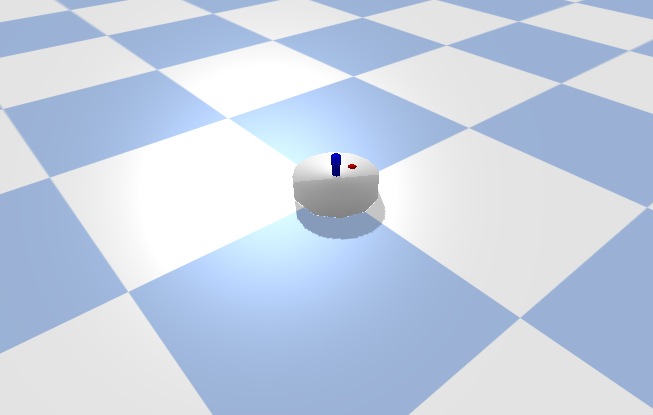
\includegraphics[width=0.8\textwidth]{figures/point_robot.png}
    \caption{The holonomic point robot the 2 velocity\\inputs drive the robot in \gls{x} and in \gls{y} direction}%
    \label{subfig:example_point_robot}
    \end{subfigure}%
    \begin{subfigure}{.5\textwidth}
    \centering
    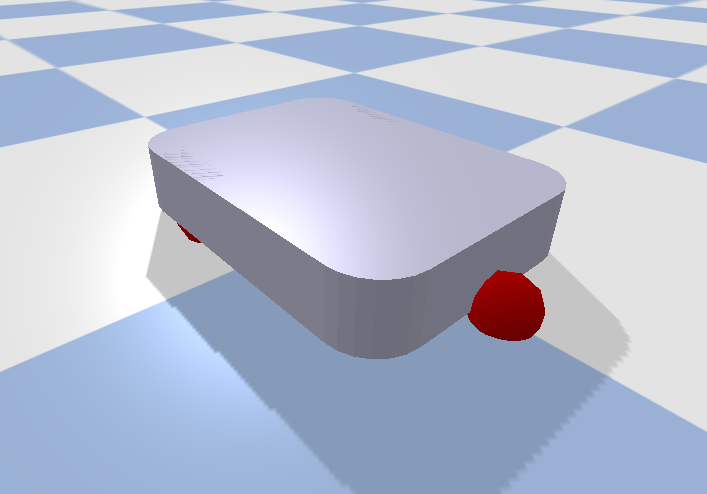
\includegraphics[width=0.8\textwidth]{figures/boxer_robot.png}
    \caption{The nonholonomic boxer robot, the\\first velocity input drives the robot forward\\ or backward the second rotates the robot}%
    \label{subfig:example_boxer_robot}
    \end{subfigure}%
    \caption{Robots used for testing the proposed method}%
    \label{fig:example_robots}
\end{figure}

\begin{figure}[H]
    \centering
    \begin{subfigure}{.5\textwidth}
    \centering
    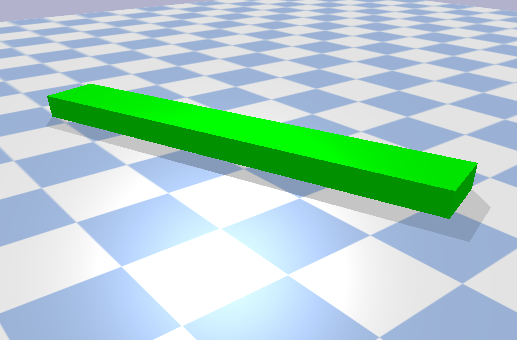
\includegraphics[width=0.8\textwidth]{figures/box_object.png}
    \caption{A box object}
    \end{subfigure}%
    \begin{subfigure}{.5\textwidth}
    \centering
    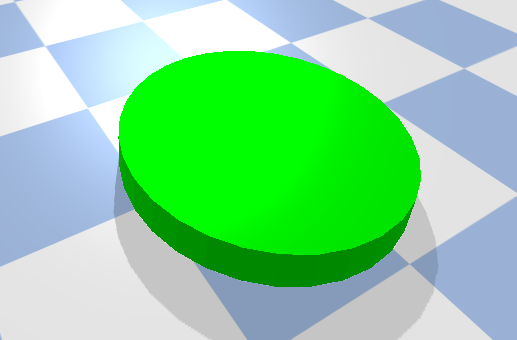
\includegraphics[width=0.8\textwidth]{figures/cylinder_object.png}
    \caption{A cylinder object}
    \end{subfigure}%
    \caption{Various objects in the robot environment}%
    \label{fig:example_objects}
\end{figure}

For complete environments with accompanying tasks, see~\Cref{chap:results}.\bs

\section{Report Structure}%
\label{sec:report_structure}
The proposed method heavily relies on a number of methods and functions. These methods and functions are conveniently grouped in \Cref{chap:required_background}. Then the proposed method is presented and discussed in \Cref{chap:hgraph_and_kgraph}. The proposed method is followed by a chapter committed to testing the proposed method, presented in \Cref{chap:results}. The last chapter dedicates itself to drawing conclusions on tests and answering the research questions in \Cref{chap:conclusion}.\bs

\chapter{Planning in Four Subspaces}%
\label{chap:proposed_planning}
\textit{This chapter presents an existing motion planner~\cite{chen_fast_2018} that is extended to incorporate movable and unknown spaces next to the conventional free and obstacle spaces. The modification incentivizes the planner to find a path in free space but can pass through unknown or movable space as a last resort. The robot should first remove the blocking objects if a planned path crosses an unknown or movable subspace.\bs}

Finding a path between the start- and target configuration whilst avoiding collisions was presented in previous chapter. Now that path planner is modified; the modification extends the planner to incorporate movable and unknown space. The modified algorithm has four tuning parameters that can be tweaked; The \textit{step size} and \textit{search size} were discussed in previous chapter. The third and fourth tuning parameters are the fixed costs for crossing through movable or unknown space. These cost are added to the \textit{TotalPathCost}, which is redefined as:\bs

\[\mathit{Cost_{path}} = \mathit{MovableSpaceCost} + \mathit{UnknownSpaceCost} \sum_{i=1}^{n-1} \mathit{Distance}(\gls{c}_i, \gls{c}_{i+1})\]
\todo{In the pseudoce you talk about objectCost, here totalpathCost, unclear!}

The \textit{MovableSpaceCost} and \textit{UnknownSpaceCost} correspond to a fixed addition cost for a configuration in the path that crosses through movable or unknown subspace, respectively. Crossing through is defined as one or more nodes in the path lying in that subspace. If a path does not contain a node in movable space, \textit{MovableSpaceCost} will be 0, equivalent to unknown space and \textit{UnknownSpaceCost}. Optimizing the path for the lowest cost incentives the path planning algorithm to find a path around unknown or movable objects.\bs

The added fixed cost for a path crossing through a movable or unknown object motivates the path planner to find the shortest path around objects but prefers moving an object over making a large detour. Tuning the additional fixed cost for a path crossing through movable or unknown space balances the robot's decision between the length of a detour the robot is willing to drive, compared to pushing an object to free the path. Removing an unknown object bears more uncertainty than a movable object, motivating a higher cost to remove an unknown object compared to an known object. In the following pseudocode for the modified path planner is presented, changes compared to previously shown pseudocode are indicated in red.\bs

The proposed algorithm prevents planning a path through blocking objects except when no other option is available or a large detour can be prevented. No performance tests have been conducted on the modified path planner, apart from visual inspection. \Cref{fig:mp_push_or_drive} clearly shows the effect of varying \textit{UnknownSpaceCosts}.

\newpage
\todo{eleborate on the change compared to the previous existing algorithm}
\todo{Dubble check if only the parts in red are changed.}
\begin{algorithm}[H]
  \caption{Pseudocode for modified \ac{RRT*} path planning algorithm. Lines that contain changes compared to \Cref{pseudocode:proposed_rrt_star_all} are indicated with the red colour.}%
  \label{pseudocode:modified_proposed_rrt_star}
  \begin{algorithmic}[1]
    \State $\gls{nodesMP} \leftarrow x_{init}$
    \While{\textit{NotReachStop}}
        \State $\gls{nodeMP}_\mathit{rand} \leftarrow \mathit{Sample_{random}}$ \algorithmiccomment{Create, project and validate a new random sample}
      \State $\gls{nodeMP}_\mathit{nearest} \leftarrow \mathit{Nearest(\gls{nodeMP}_{rand}, \gls{nodesMP})}$
      \State $\gls{nodeMP}_\mathit{temp} \leftarrow \mathit{Project(\gls{nodeMP}_{rand}, \gls{nodeMP}_{nearest})}$
      \If{$\mathit{CollisionCheck(\gls{nodeMP}_{temp})}$}
      \State $\gls{nodeMP}_\mathit{new} = \gls{nodeMP}_\mathit{temp}$
      \State $\mathit{Cost_{toInitMin}} \leftarrow +\infty$ 
      \Else
      \State Continue
      \EndIf
      \State $X_\mathit{near} \leftarrow \mathit{NearestSet(\gls{nodeMP}_{new}, \gls{nodesMP})}$ \algorithmiccomment{Find and connect new node to parent node}
      \For{$\gls{nodeMP}_\mathit{near} \in X_\mathit{near}$}
    \State $\mathit{Cost_{temp}} \leftarrow \mathit{CostToInit}(\gls{nodeMP}_\mathit{near}) + \mathit{Distance}(\gls{nodeMP}_\mathit{near}, \gls{nodeMP}_\mathit{new}) + \textcolor{red}{\mathit{ObjectCost}(\gls{nodeMP}_\mathit{near}, \gls{nodeMP}_\mathit{new})}$
      \If{$\mathit{Cost_{temp}}  < \mathit{Cost_{toInitMin}}$}
      \State $\mathit{Cost_{toInitMin}} \leftarrow \mathit{Cost_{new}}$
      \State $\gls{nodeMP}_\mathit{minCost} \leftarrow \gls{nodeMP}_\mathit{near}$
      \EndIf
      \EndFor
      \If{$\mathit{Cost_{toInitMin}} == \infty$}
          \State Continue
      \Else
      \State $\gls{nodesMP}.add(\gls{nodeMP}_\mathit{new})$
      \State $E.\mathit{add}(\gls{nodeMP}_\mathit{minCost}, \gls{nodeMP}_\mathit{new})$
      \EndIf
      \State $\mathit{Cost_{pathMin}} \leftarrow +\infty$ 
      \For{$\gls{nodeMP}_\mathit{near} \in X_{near}$}\algorithmiccomment{\parbox[t]{.6\linewidth}{Check if the newly added node can lower cost for nearby nodes and if a both connectivity trees can be connected}}
      \If{$\mathit{InSameTree(\gls{nodeMP}_{near}, \gls{nodeMP}_{new})}$}
    \If{$\mathit{CostToInit(\gls{nodeMP}_{new})} + \mathit{Distance(\gls{nodeMP}_{new}, \gls{nodeMP}_{near})} +\textcolor{red}{\mathit{ObjectCost}(\gls{nodeMP}_\mathit{new}, \gls{nodeMP}_\mathit{near})} < \mathit{CostToInit(\gls{nodeMP}_{near})}$}
      \State $\mathit{E.rewire(\gls{nodeMP}_{near}, \gls{nodeMP}_{new})}$
      \EndIf
      \Else \algorithmiccomment{Add lowest cost path to the list of paths}

      \State $\mathit{Cost_{temp} \leftarrow CostToInit(\gls{nodeMP}_{new}) + Distance(\gls{nodeMP}_{new}, \gls{nodeMP}_{near})} + \mathit{CostToInit(\gls{nodeMP}_{near})}$
      % \State $\mathit{Cost_{temp} \leftarrow CostToInit(\gls{nodeMP}_{new}) + Distance(\gls{nodeMP}_{new}, \gls{nodeMP}_{near})} + \mathit{CostToInit(\gls{nodeMP}_{near}) + \textcolor{red}{ObjectCost(\gls{nodeMP}_{new}, \gls{nodeMP}_{near})}}$
      \If{$\mathit{Cost_{temp}  < Cost_{pathMin}}$}
      \State $\mathit{Cost_{pathMin}} \leftarrow \mathit{Cost_{temp}}$
      \State $\mathit{\gls{nodeMP}_{pathMin} \leftarrow \gls{nodeMP}_{near}}$
      \EndIf
      \EndIf
      \If{$Cost_{pathMin} == \infty$}
      \State Continue
      \Else
      \State $\mathit{P.addPath(\gls{nodeMP}_{new}, \gls{nodeMP}_{pathMin}, Cost_{pathMin})}$
      \EndIf
      \EndFor
    \EndWhile
  \end{algorithmic}
\end{algorithm}

\begin{figure}[H]
    \centering
    \begin{subfigure}{\textwidth}
    \centering
    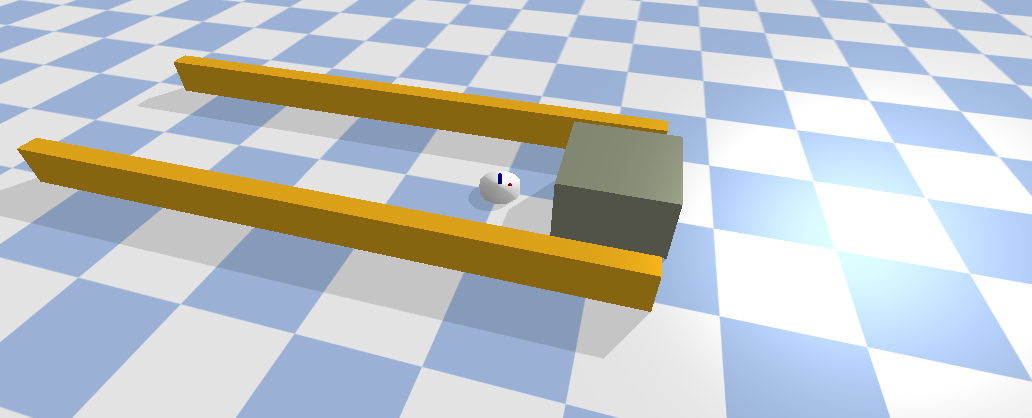
\includegraphics[width=0.8\textwidth]{figures/required_background/push_or_drive} \caption{Robot environment with the point robot, two yellow unmovable walls and an unknown brown box.\\The robot tasked to drive toward the opposite side of the brown box.}

\todo{Could you at least place a ghost pose on in this figure?}

    \end{subfigure}

    \begin{subfigure}{1.11\textwidth}
    \centering
    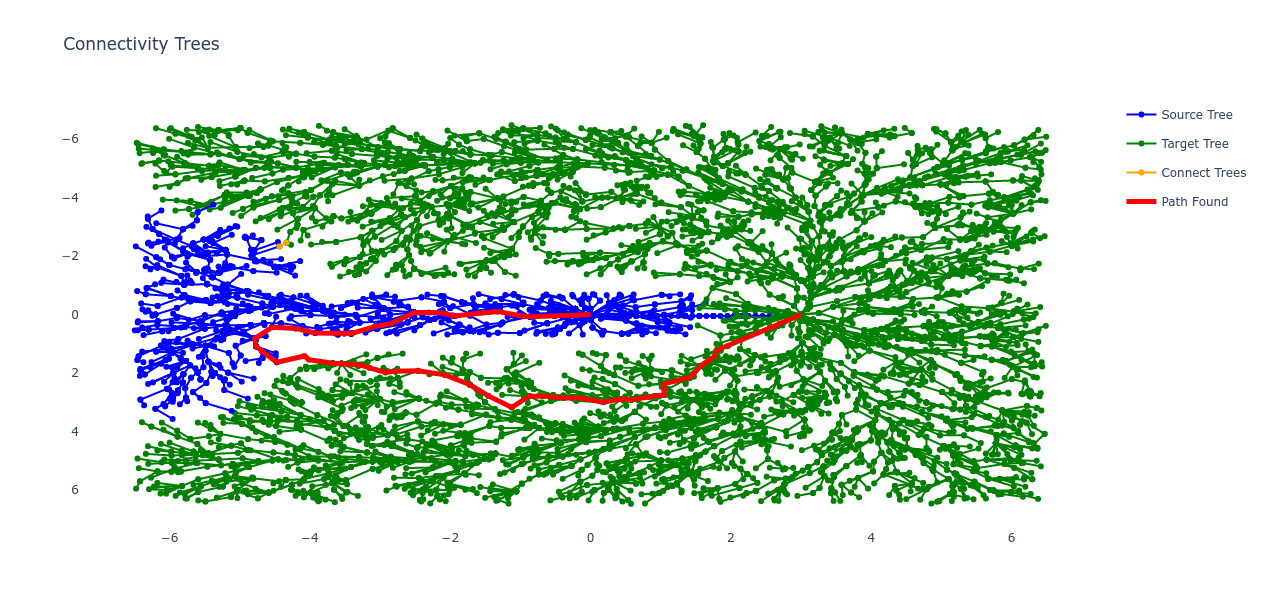
\includegraphics[width=\textwidth]{figures/required_background/mp/mp_high_fixed_cost}
    \caption{Visualization of the planned path around the brown box and yellow obstacles, with $\mathit{UnknownSpaceCost} = 1$.}
    \end{subfigure}

    \begin{subfigure}{1.11\textwidth}
    \centering
    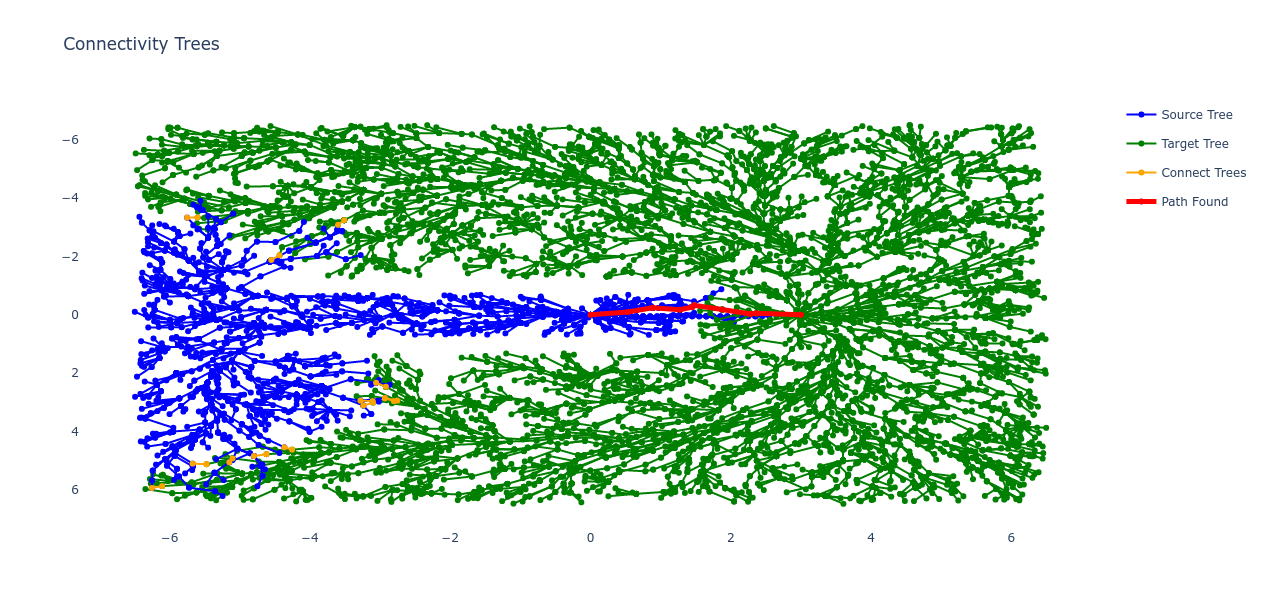
\includegraphics[width=\textwidth]{figures/required_background/mp/mp_low_fixed_cost}
    \caption{Visualization of the planned path going through the brown box, $\mathit{UnknownSpaceCost} = 0.5$.}
    \end{subfigure}
    \caption{Driving task and two path planned by the modified planning algorithm.}%
    \label{fig:mp_push_or_drive}
\end{figure}

Now that the modified path planner is discussed, the proposed robotic framework is discussed. The proposed framework relies on the required background from previous chapter, and relies on the modified path planner from this chapter.\bs



\todo{create a test that does things for the boxer robot, and it must have non-holonomic checker residing in the path}


% old manipulation section shit

% \subsection{Manipulation Planning}%
% \label{subsec:manipulation_planning}
% With a push, two objects are primarily involved, the pushed object and the robot. Generally, and in this thesis, the pushed object's configuration is more important than the robot's configuration. The robot is only a means to push the object toward the target configuration. At which final configuration the robot itself ends up is of lesser importance. As long as during the push, the robot does not collide with objects other than the pushed object, and constraints on the robot must be respected.\bs

% To plan a path that respects the constraints, \todo{Corrado: What does this mean? ->} the robot's configuration is generated for every newly added sample in the manipulation planning algorithm.

% \todo{Gijs For reachbailbpcheck, These lines just point out the name of the function again , there is no added information }
% The \textit{ReachabilityCheck()} (see \Cref{table:functions_for_proposed_rrt_star} and line 33 in \Cref{pseudocode:proposed_rrt_star}) generates the robot configuration to validate if a new sample is reachable from an existing sample. This additional configuration is stored to create only feasible paths that respect the applied constraints. When the stopping criteria are reached and the shortest path is found, the generated robot configurations are discarded. \Cref{fig:manipulation_plannig_local_planner} displays a visual example of the procedure.\bs

% \begin{figure}[H]
%     \centering
%     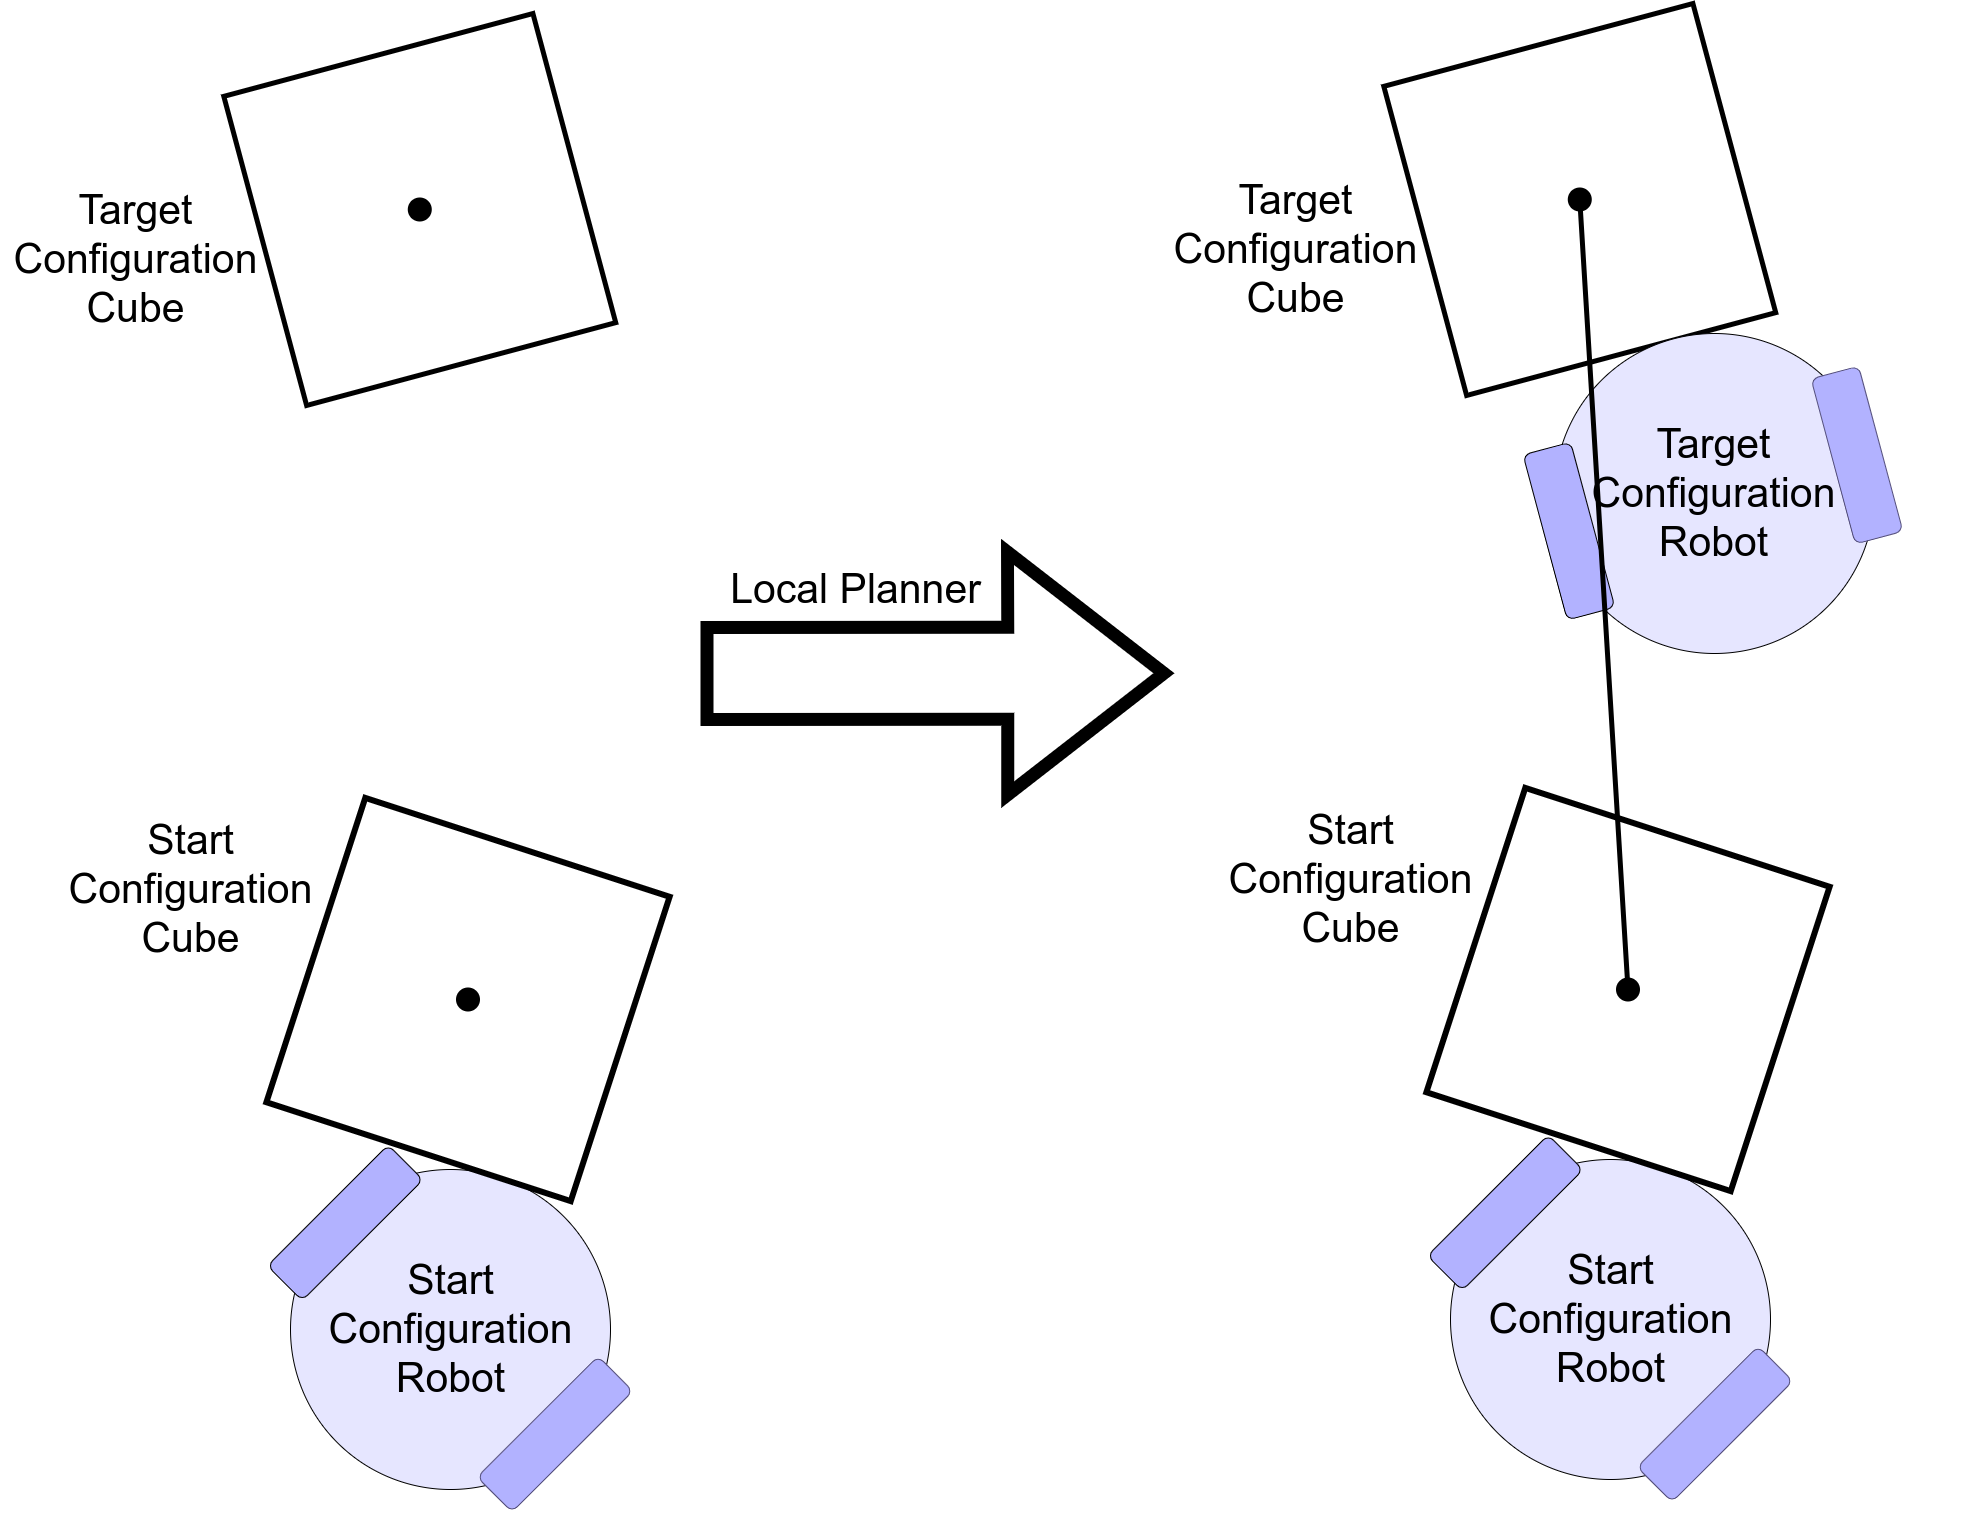
\includegraphics[width=0.6\textwidth]{figures/required_background/manipulation_local_planner}
%     \caption{Generating a new robot configuration whilst adding a sample to the connectivity tree during manipulation planning.}%
%     \label{fig:manipulation_plannig_local_planner}
% \end{figure}

 
\chapter{Proposed Robot Framework}%
\label{chap:h-graph_and_k-graph}
\textit{This chapter is dedicated to introducing and defining the proposed framework. The proposed framework consists of the \textbf{\acf{h-algorithm}}, the \textbf{\acf{h-graph}} and the \textbf{\acf{k-graph}}. The \ac{h-algorithm} acts on the \ac{h-graph} and is responsible for searching and executing action sequences to complete a specified task. \Cref{sec:h-graph} is dedicated to introducing and defining the \ac{h-graph}. Then the \ac{h-algorithm} is discussed and defined in \Cref{sec:h-algorithm}. The chapter finalizes with the \ac{k-graph} in \Cref{sec:k-graph}.\bs}

\section{Overview of the Proposed Framework}
\Cref{tikz:flowchart_proposed_method} presents a schematic overview of the interconnection of the \ac{k-graph}, \ac{h-algorithm} and the robot environment. The proposed framework could be augmented with a high-level planner that would transform a high-level task such as cleaning into the accepted format a list containing objects and corresponding target pose.\bs

\vspace{-0.4cm}
\begin{figure}[H] \centering
\begin{tikzpicture}[node distance = 1.5cm, auto]
    % Place nodes
    \node[draw=gray, rounded corners, inner sep=3ex, line width=7pt, fill=gray, fill opacity=0.4, minimum height=9.3cm, minimum width=5.8cm, yshift=2.50cm] (focusbox) {};
    \node[yshift=5.0cm, xshift=-1.5cm, align=left] at (focusbox) {\textbf{Thesis focus}};

   \node [outer sep=0cm] (environment) at (0,0)  {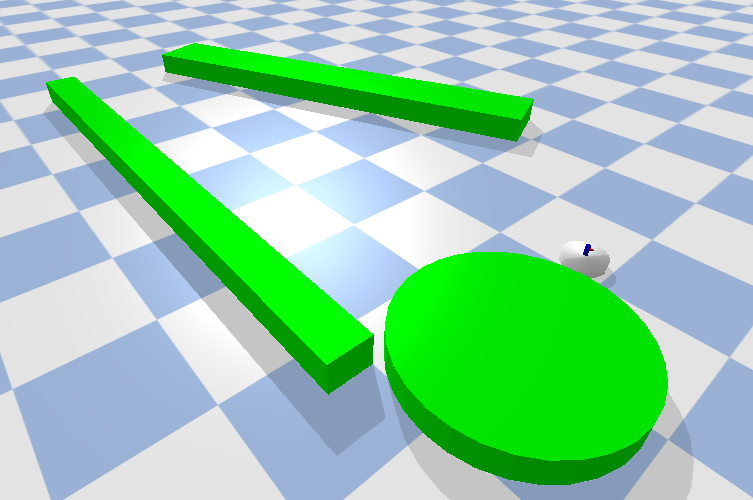
\includegraphics[width=4.6cm]{figures/proposed_method/example_environment.png}};

   \node [below, xshift=0.4cm, yshift=-.1cm, text width=5cm, align=left, outer sep=0cm] at (environment.north) {\textbf{Robot Environment}};

    \draw [myEvenLighterColor,
    rounded corners=0.3cm,
    line width=0.3cm]
    (environment.north west) --
    (environment.north east) --
    (environment.south east) --
    (environment.south west) -- cycle  ;

    \node [block,
    above of=environment,
    minimum height=1.5cm,
    minimum width=5cm,
    node distance=3.6cm,
    outer sep=0cm] (h-graph) {Hypothesis Algorithm};

    \node [block,
    above of=h-graph,
    node distance=2.5cm,
    minimum width=5cm,
    minimum height=1.5cm] (k-graph) {Knowledge Graph};

    \node [rectangle, draw,
    fill=myEvenLighterColor,
    text width=5em, text centered, rounded corners,
    right of=k-graph,
    minimum width=4cm,
    minimum height=1.5cm,
    node distance=7.5cm] (ontology) {Ontology};

    \node [rectangle, draw,
    fill=myEvenLighterColor,
    text width=5em, text centered, rounded corners,
    right of=h-graph,
    minimum width=4cm,
    minimum height=1.5cm,
    node distance=7.5cm] (planner) {High-level planner};

    % Draw edges
    \draw[-stealth] ([yshift=0.155cm, xshift=0.3 cm]environment.north) -- node [xshift=-.05cm, right] {\shortstack[]{sensor\\measurements}}([xshift=0.3 cm]h-graph.south) ;
    \draw[-stealth] ([xshift=-0.3 cm]h-graph.south) -- node [left] {robot input}([yshift=0.155cm, xshift=-0.3 cm]environment.north) ;
    \draw[-stealth] (planner.west) -- node [pos=0.37, above] {task}(h-graph.east);
    \draw[-stealth] ([xshift=-0.3cm]k-graph.south) -- node [left] {\shortstack[]{action\\suggestions}}([xshift= -0.3cm]h-graph.north) ;
    \draw[stealth-] ([xshift=0.3cm]k-graph.south) -- node [right] {\shortstack[]{action\\feedback}}([xshift= 0.3cm]h-graph.north) ;
    \draw[-stealth] (k-graph.east) -- node [xshift=-0.1cm, above, pos=0.63] {\shortstack[]{environment\\knowledge}}(ontology.west);
    \draw[stealth-] ([xshift=0.3cm]ontology.south) -- node [right] {\shortstack[]{query}}([xshift=0.3cm]planner.north);
    \draw[-stealth] ([xshift=-0.3cm]ontology.south) -- node [left] {\shortstack[]{output}}([xshift=-0.3cm]planner.north);
    \draw[stealth-] (planner.south) |- ++ (2,-1) node[near end, above] {\shortstack[]{High-level\\task}};
    \end{tikzpicture}
\caption{Flowchart representation of the proposed robot framework.}%
\label{tikz:flowchart_proposed_method}
\end{figure}

The block containing the \ac{h-algorithm} in \Cref{tikz:flowchart_proposed_method} orchestrates the generation and execution of action sequences. In doing so, it creates a \ac{h-graph}, first the \ac{h-graph} is introduced and discussed, then the \ac{h-algorithm} is introduced and discussed.\bs

\section{Hypothesis Graph}%
\label{sec:hgraph}
The \ac{halgorithm} is responsible for generating action sequences, called hypothesis. An hypothesis consists of a list of successive edges in the \ac{hgraph} from start to target node in the \ac{hgraph}. When all subtasks in a task are completed, the \acf{halgorithm} halts and concludes the task successfully completed. A search in the joint configuration space is avoided because an edge only operates in a single mode of dynamics, such as driving or pushing. When an object cannot directly be steered toward its target location new nodes are generated which need to be completed before the original object can be steered toward its target location. An example of when an object cannot directly be steered toward its target state is because the path is blocked by another object. A hypothesis, consisting of a list of edges that represent actions in the robot environment might succeed or fail. \Cref{tikz:flowchart_hgraph} displays a flowchart explaining how new nodes and edges are generated in the \ac{hgraph}. Successfully completed edges eventually result in completed subtasks, failed edges trigger replanning that will restart the search to a hypothesis.\bs

The \ac{halgorithm} with the \ac{hgraph} have a familiar structure compared to some recent literature~\cite{ellis_navigation_2022,wang_affordancebased_2020}. An important distinction is that the proposed method in this thesis aims to combine the 3 topics: learning object dynamics, solving \ac{NAMO} problems and nonprehensile pushing. Recent literature is able to only combine one or two topics of the three.\bs

In the upcoming section the \ac{hgraph} is defined and discussed in \cref{subsec:hgraph_definition}. The \ac{halgorithm} is then discussed and in \cref{subsec:halgorithm}, where an explanation is provided on how the \ac{halgorithm} searches for a solution in the joint configuration space. The section is concluded with an extensive example.\bs

\subsection{Definition}%
\label{subsec:hgraph_definition}%
Before defining the \ac{hgraph}, some definitions are defined on which the \ac{hgraph} depends. First, recall the \textbf{state} defined in the \cref{sec:problem_description}.\bs

An object holds the information about an object.\\Formally, a \textbf{object},  $obst_{id}(k) = \left\langle s(k), shape \right\rangle $\bs

where $shape$ is linked to a 3D representation of the object which is used to construct the configuration space.\bs

An object node represents an object in a state.\\Formally, a \textbf{objectNode}, $V^{obst}_{id} =\left\langle \textrm{status}, obst(k)\right\rangle $\\where status indicates if the node has been visited in the \ac{hgraph}. $\textrm{status} = (Initialised, Completed, Failed)$\bs

An edge describes the details of how a node transitions to another node in the \ac{hgraph}. In the robot environment, an edge represents a change of state for an object. System identification and performing an action such as pushing or driving both change the state of objects in the robot environment, but because are very different, the edges are split into 2 categories. IdentificationEdges that collect system \ac{IO} data and convert that into a system model. And actionEdges that plan and track a motion from a start to a target state. Formally:\bs

A \textbf{identificationEdge},
\todo[inline]{define identificationEdge, currently hard coded models are used in the implementation}

A \textbf{actionEdge}, $\tau_{(from, to)} = \left\langle \textrm{status}, id_{from}, id_{to}, \textrm{verb}, \textrm{controller},\textrm{dynamic model}, \textrm{path}\right\rangle$\bs

with $id_{from}$ and $id_{to}$ indicating the node id of the node in the \ac{hgraph} where the edge start from and point to respectively, $verb$ an English verb describing the action the edge represents, the controller contains the controller used for driving the robot, the dynamic model is the dynamic model used by the controller, path a list of configurations indicating the path connecting a start- to target node.\bs
\todo[inline]{Martijn: what does this mean: "the controller contains the controller..."?}

A $verb = \{\textrm{driving, pushing}\}$.\bs

Now the nodes and edges have been defined, the \ac{hgraph} can be defined.\bs

Formally, a \textbf{hypothesis graph}, $G^{hypothesis} = \left\langle V, E \right\rangle $ 
\\comprising $V = \{V^{ob}_{i}\}$, \quad $E \in \{\tau_{(i,j)}| V_i, V_j \in \{V^{ob} \}, i \neq j\}$.\bs

Most \ac{hgraph} components have now been defined. The status of an identification edge or action edge still remains undefined and requires some further explanation.\bs

\paragraph{Status, Types and Lifetime of edges}
Because system identification and tracking a path are so very different, the edges are split into two categories, identification edges and action edges. An identification edge, which is responsible for sending an input sequence to the system and recording the system output. That input/output sequence and assumptions on the system are the basis for system identification, techniques on various system identification methods are discussed in \cref{sec:sys_iden}. The goal is to create a dynamical model which is augmented with a corresponding controller is closed-loop stable.\bs

An identificationEdge, the status can be visualised in \cref{tikz:status_identification_edge}.\bs

\begin{figure}[H]
\centering
\begin{tikzpicture}[node distance = 2cm, auto, initial]
    \node [state, fill=my_dark_blue] (init_test_num) {IT\#t};
    \node [state, fill=my_light_blue, below of=init_test_num] (completed_test_num) {CT\#t};
    \node [state, accepting, fill=my_green, below of=completed_test_num] (completed) {CO};
    \node [state, accepting, fill=my_red, right of=completed_test_num, node distance=6cm] (failed) {FAIL};

 % arrows
    \draw [-stealth] ([xshift=-2cm]init_test_num.west) to node[near start,above]{\shortstack[]{select compatible\\sys. iden. method}} (init_test_num.west);
    \draw[-stealth] (init_test_num) edge[bend right] node[left]{Collect \ac{IO} data} (completed_test_num)
(completed_test_num) edge node[left]{create system model} (completed);
    \draw [-stealth] (completed_test_num) edge[bend right] node[right]{goto next start state} (init_test_num);
    \draw [-stealth] (completed_test_num) to node[]{Unable to reach next start state}  (failed.west);
    \draw [-stealth] (init_test_num) [out=0, in=90] to node[above]{Unable to reach next pos}  (failed.north);

\end{tikzpicture}
\caption{\acs{FSM} displaying the status of an identification edge}%
\label{tikz:status_identification_edge}
\end{figure}

\todo[inline]{some explainer on this status of iden edge}

The second type of edge is an actionEdge, containing a drive or push action. An actionEdge ready for execution contains all the necessary information to send input to the robot resulting in an object being steered toward it's target state. Before an edge is ready for execution it should be initialised properly, more specifically: initialised, path estimated should be performed, a system model must be initiated and path planning must be performed. Then finally the edge is ready to be executed and send input toward the robot, an \ac{FSM} of the actionEdge's status can be visualised in \cref{tikz:status_action_edge}.\bs

\begin{figure}[H]
\centering
\begin{tikzpicture}[node distance = 2cm, auto, initial]
    % \node [state, fill=lavenderIndigo] (init) {IN};
    \node [state, fill=my_purple] (init) {IN};
    \node [state, fill=my_dark_blue, below of=init] (path_exist) {PE};
    \node [state, fill=my_light_blue, below of=path_exist] (system_model) {SM};
    \node [state, fill=my_green, below of=system_model] (path_planned) {PP};
    \node [state, fill=my_yellow, below of=path_planned] (executing) {EX};
    \node [state, accepting, fill=my_orange, below of=executing] (completed) {CO};
    \node [state, accepting, fill=my_red] (failed) at ([xshift=4cm]$(system_model)!0.5!(path_planned)$) {FAIL};
    
 % arrows
    \draw [-stealth] ([xshift=-2cm]init.west) to node[near start,above]{select controller} (init.west);
    \draw[-stealth] (init) edge node[left]{graph-based path estimation} (path_exist)
      (path_exist) edge[bend right] node[left]{load in system model} (system_model)
(system_model) edge[bend right] node[left]{motion planning} (path_planned)
(path_planned) edge[bend right] node[left]{goto execution loop} (executing)
(executing) edge[bend right] node[left]{completed} (completed);

    \draw [-stealth] (init.east) [out=0, in=90] to node[xshift=0.1cm, right]{path non-existence proven}  ([yshift=-0.03cm,xshift=0.2cm]failed.north);
    \draw [-stealth] (path_exist.east) [out=0, in=90] to node[xshift=-0.6cm,yshift=0.55cm, above]{\shortstack[l]{system\\identification\\error}}  ([yshift=-0.03cm,xshift=-0.2cm]failed.north);
    \draw [-stealth] (system_model.east) [out=0, in=180] to node[xshift=0.1cm, yshift=0.3cm, above]{\shortstack[l]{motion\\planning\\error}} (failed.west);
    node[right]{motion planning error}  
    ([yshift=-0.3cm]failed.west);
    \draw [-stealth] (executing.east) [out=0, in=-90] to node[xshift=0.1cm,right]{fault detected}(failed.south);

\end{tikzpicture}
\caption{\acs{FSM} displaying the state of an action edge}%
\label{tikz:status_action_edge}
\end{figure}

% \par\smallskip\noindent
\centerline{\begin{minipage}{0.8\textwidth}
\begin{enumerate}
  \item[INITIALISED (IN)] The edge is created with a source and target node which are present in the \ac{hgraph}. A choice of controller is made.
    \item[PATH EXISTS (PE)] A graph-based search is performed to validate if the target state is reachable assuming that the system is holonomic.
    \item[SYSTEM MODEL (SM)] A dynamics system model is provided to the controller residing in the edge.
    \item[PATH PLANNED (PP)] Resulting from a sample-based planner, a path from start to target state is provided. 
    \item[EXECUTING (EX)] The edge is currently receiving observations from the robot environment and sends back robot input. 
    \item[COMPLETED (COMPL)] The edge has driven the system toward its target state and its performance has been calculated.
    \item[FAILED (FAIL)] An error occurred, yielding the edge unusable. 
\end{enumerate}
\end{minipage}}
\par\smallskip

\Cref{tikz:status_action_edge} shows that many steps must successfully be completed before the robot can start executing. The performance of an edge during execution, measured in various metrics (\cref{sec:proposed_method_metrics} is dedicated to metrics) is dependent on many aspects. Such as the choice of controller, the path estimation, the system model yielded by the identification edge and the path yielded by motion planning. Now that he \ac{hgraph} is defined, let's see how it is generated in the upcoming section.\bs

\subsection{\acl{halgorithm}}%
\label{subsec:halgorithm}
This section will provide a mathematical description of the proposed \ac{halgorithm}, the search and execution loop are discussed. The section will finalise with 4 examples. First, let's look into the math of the \ac{halgorithm}.\bs

\todo[inline]{a mathematically solid describtion of your backward search algorithm}

During a backward search, edges are added pointing toward the target node (or to nodes that point toward the target node). Trying to connect the robot node through a list of succesive directed edges to a target node. If such a path has been found in the \ac{hgraph}, a hypothesis has been found and the robot can start executing edges.

A flowchart of the \ac{halgorithm} is presented in \cref{tikz:flowchart_hgraph}. Compared to the mathematical description of the \ac{halgorithm} the flowchart provides more detail, including an eleborate description for every block in the flowchart (see \cref{table:explainer_hgraph_figures_nodes}). The flowchart includes path estimation, planning and the behavior when failure occures. A connection point to the \ac{kgraph} and robot environment are included. The blocks in the flowchart indicate which action they take and where, such as the configuration space, the \ac{kgraph} or the \ac{hgraph}. With the flowchart is straigtforward to see how the \ac{halgorithm} connects to the status of edges, with the mathematical description of the \ac{halgorithm} that is harder so see. Compared to the flowchart the mathematical description is a abstacted version, leaving many details out that are related to the robot in this thesis. An abstracted mathematical description is simpler and encompasses a broader field of robots. So could the mathematical description also be applied to another robot such as a movable robot with robot arm and gripper. The flowchart encompasses to many details to be applied after such an change in robot hardware. 

\input{mainmatter/hypothesis_graph/hgraph_tikz_figure}

\begin{table}[H]
\centering
\rowcolors{2}{white}{myLightColor}
\begin{tabular}[t]{>{\raggedright}p{3.5cm}>{\raggedright\arraybackslash}p{10.5cm}}
  \textbf{Node name} & \textbf{Description of actions taken}\\\toprule
  Task Finished & log all metrics for the \ac{hgraph}, then deconstruct \ac{hgraph}.\\
  Create Start and\newline Target Nodes & Generate a robot node and the start and target nodes for every subtask in the task.\\
Update Current Subtask & Select an unfinished subtask or update current subtask. Use the backward search technique. The \textit{current\_start\_node} and \textit{current\_target\_node} are updated. When all subtask have been addressed, conclude task is finished. \\
Estimate Path\newline Existence & Check if a path exists between \textit{current\_start\_node} and \textit{current\_target\_node} whilst assuming that the object is holonomic.\\
Add Node to\newline Drive to Object & Add a node before the \textit{current\_target\_node}.\\
Unfeasible Node & Update node's status to unfeasible because is can not be completed, log failed Edge.\\
Knowledge Available& Query the \ac{kgraph} for action suggestion to connect \textit{current\_target\_node} to \textit{current\_target\_node}\\
Knowledge Usable& Check if a suggested action is not on the blacklist.\\
Object Movable & Check if object is classified as movable\\
Robot Close to Object& Check if the object is inside directly reachable free space of the robot \\
Generate Random\newline Action& Randomly sample a controller with a compatible system identification method that is not on the blacklist. \\
All Possible Actions Failed & Every possible action is on the blacklist for the \textit{current\_target\_node}, update \textit{current\_target\_node} status to failed.\\
Add Drive System Identification Edge & Adds identification edge between a newly generated node and the drive action edge source node. \\
Model Available& Checks if the drive action edge contains a system model. \\
Action Type& Checks the action type. \\
Model Available& Checkif the push action edge containts a system model. \\
Add Push System\newline Identification Edge& Adds identification edge compatible with push action edge. \\
Motion Planning& Search a path for the \textit{current\_edge}, detect blocking objects. \\
Add Node to Free Path & Search closeby pose for object to free path. Create node to push object toward that pose. \\
Manipulation Planning & Search a path for the \textit{current\_edge}, detect blocking objects.\\
Add Node to Drive\newline to Push Pose& Create node to drive toward push pose, add before action edge. \\
Robot Close to\newline Push Pose & Check if the robot is overlapping with the best push position. \\
Path to Target& Is there a path from robot to target node in the \ac{hgraph}, then set first edge to \textit{current\_edge} otherwise update subtask.\\
First Action Planned&  Check if motion/manipulation planning was performed. \\
Execute& Execute the \textit{current\_edge}, update \ac{hgraph} after completion, log failed hypothesis if a fault is detected. \\
Subtask Succesfully\newline Completed& Log hypothesis metrics. \\
Target Node Reached& Check if the target node is reached.\\
\end{tabular}
\caption{Eleborate information on actions taken by blocks in \cref{tikz:flowchart_hgraph}.}%
\label{table:explainer_hgraph_figures_nodes}
\end{table}

When all tuning parameters are set, the \ac{hgraph} is initialized and a task is provided, there is only a single access point toward the \ac{hgraph}. A function \textit{respond(observation)} that provides the \ac{halgorithm} with sensor measurements of the environment with the argument \textit{observation}. The function \textit{respond($\cdot$)} returns control in put for the robot. In this theses, the sensor measurements are the configuration of objects in the environment. Recall that the perfect-sensor assumption, assumption~\ref{assumption:perfect_object_sensor} that makes access to the exact configuration of every object possible.\bs


\paragraph{The Blacklist}%
Undesirable behavior is to generate an edge that fails, only to regenerate and fail again. This infinite behavior is prevented by the blacklist. When the \ac{halgorithm} connects two nodes with an action edge, the possible parameterizations (controller and system model) are filtered. Thus any parameterisation that is on the blacklist for this specific node (to which the action edge would point toward) cannot be created again for the lifetime of the \ac{hgraph}. An example where the blacklist can be seen in action is \cref{fig:failure_in_hgraph}.\bs

\todo[inline]{math def for blacklist on the nodes}


\subsection{The Search and the Execution loop}%
\label{subsec:two_loops}
In \cref{tikz:flowchart_hgraph} two main loops can be identified, see \Cref{fig:two_loops_identified}. These loops are the search loop, and the execution loop.\bs

\begin{figure}[H]
    \centering
    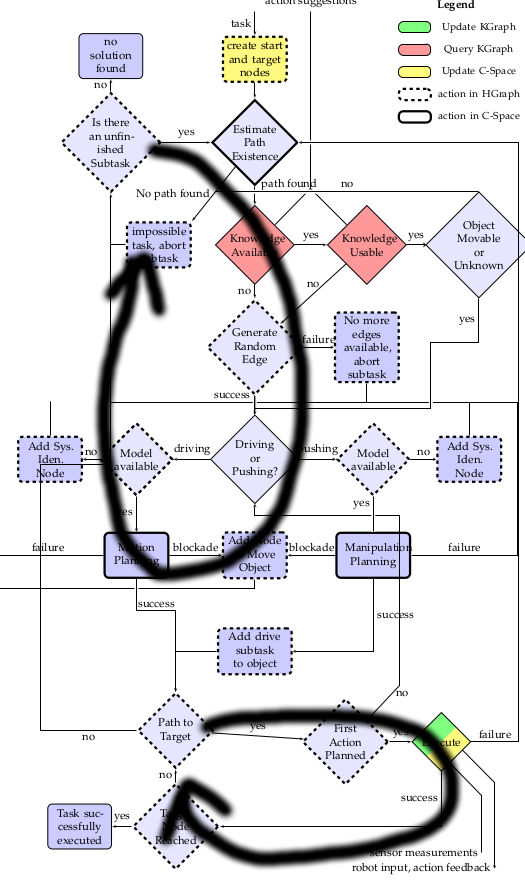
\includegraphics[width=7cm]{figures/two_loops_identified}
    \caption{The search (above) and execution (below) loop.}%
    \label{fig:two_loops_identified}
\end{figure}

Whilst the \ac{halgorithm} resides in the search loop, hypotheses are formed. Forming a hypothesis generates nodes, edges, and progressing their status as described in \cref{tikz:status_identification_edge,tikz:status_action_edge}. In the execution loop \textit{an edge is being executed}, a phrase to describe that the controller residing in an edge is sending control input toward the robot. The \ac{halgorithm} operates synchronously, thus at any point in time, the \ac{halgorithm} resides in a single block within \cref{tikz:flowchart_hgraph}. The result is that the robots cannot operate whilst the \ac{halgorithm} resides in the search loop, and during execution, no hypothesis can be formed or updated. Assumption~\ref{assumption:closed_world} guarantees that the robot environment does not change causing existing hypotheses to be outdated.\bs

\subsection{Examples}%
\label{subsec:hgraph_example}

Before displaying example \ac{hgraph}'s a legend is now presented.\bs

\begin{figure}[H]
    \centering
    \begin{subfigure}{0.2\textwidth}
    \centering
    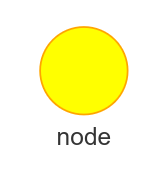
\includegraphics[width=0.7\textwidth]{figures/connecting_nodes/legend/node}
    \caption{Regular node created by the \ac{halgorithm}.\newline}%
    \end{subfigure}
    \begin{subfigure}{0.2\textwidth}
    \centering
    
\includegraphics[width=0.7\textwidth]{figures/connecting_nodes/legend/current_node}
    \caption{Current node indicates that it's outgoing edge is now or is next to be executed.}%
    \end{subfigure}
    \begin{subfigure}{0.2\textwidth}
    \centering
    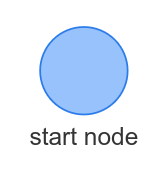
\includegraphics[width=0.7\textwidth]{figures/connecting_nodes/legend/starting_node}
    \caption{Starting node, one is generated at for every subtask.}%
    \end{subfigure}
    \begin{subfigure}{0.2\textwidth}
    \centering
    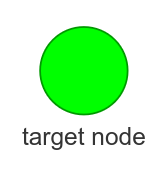
\includegraphics[width=0.7\textwidth]{figures/connecting_nodes/legend/target_node}
    \caption{Target node, one is generated for every subtask.\newline}%
    \end{subfigure}

    \begin{subfigure}{0.33\textwidth}
    \centering
    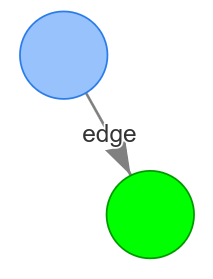
\includegraphics[width=0.7\textwidth]{figures/connecting_nodes/legend/edge}
    \caption{Edge with status IN, PE, SM, PP or EX.}%
    \end{subfigure}
    \begin{subfigure}{0.33\textwidth}
    \centering
    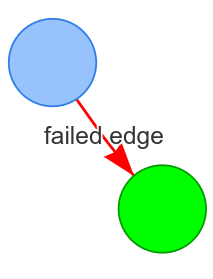
\includegraphics[width=0.7\textwidth]{figures/connecting_nodes/legend/failed_edge}
    \caption{Edge with status FAILED (FAIL)}%
    \end{subfigure}
    \begin{subfigure}{0.33\textwidth}
    \centering
    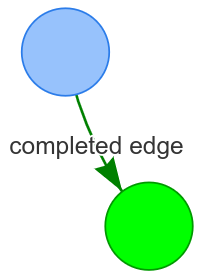
\includegraphics[width=0.7\textwidth]{figures/connecting_nodes/legend/completed_edge}
    \caption{Edge with status COMPLETED (CO)}%
    \end{subfigure}
    \caption{Legend for \ac{hgraph}'s nodes an edges}%
    \label{fig:hgraph_legend}
\end{figure}

\paragraph{Driving and Pushing} Four examples are presented, starting with a driving task in \cref{fig:robot_drive_hgraph}, then a pushing task in \cref{fig:robot_push_hgraph}.\bs

\begin{figure}[H]
    \centering
    \begin{subfigure}{.3\textwidth}
    \centering
    \includegraphics[width=0.7\textwidth]{figures/connecting_nodes/robot_to_target/robot_to_target}
    \end{subfigure}
    \begin{subfigure}{.3\textwidth}
    \centering
    \includegraphics[width=0.9\textwidth]{figures/connecting_nodes/robot_to_target/robot_drive_target}
    \end{subfigure}
    \begin{subfigure}{.3\textwidth}
    \centering
    \includegraphics[width=\textwidth]{figures/connecting_nodes/robot_to_target/robot_iden_drive_target}
    \end{subfigure}
    \caption{\ac{hgraph} generated by the \ac{halgorithm} to drive the robot to a target configuration}%
    \label{fig:robot_drive_hgraph}
\end{figure}

The robot does not have a system model of itself, thus first system identification must be performed before it can drive to the specified target configuration. The \ac{kgraph} that will be discussed in \cref{subsec:kgraph_definition} can suggest an action that includes a system model. In that case, system identification is not needed. The following figure displays succesfully executing the hypothesis found in \cref{fig:robot_drive_hgraph}.\bs

\begin{figure}[H]
    \centering
    \begin{subfigure}{.3\textwidth}
    \centering
    \includegraphics[width=0.8\textwidth]{figures/connecting_nodes/robot_to_target/execute_robot_to_target_1}
    \end{subfigure}
    \begin{subfigure}{.3\textwidth}
    \centering
    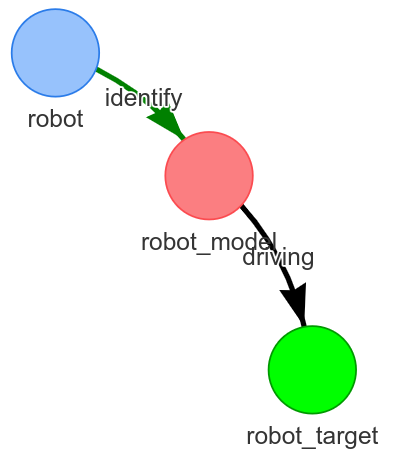
\includegraphics[width=0.8\textwidth]{figures/connecting_nodes/robot_to_target/execute_robot_to_target_2}
    \end{subfigure}
    \begin{subfigure}{.3\textwidth}
    \centering
    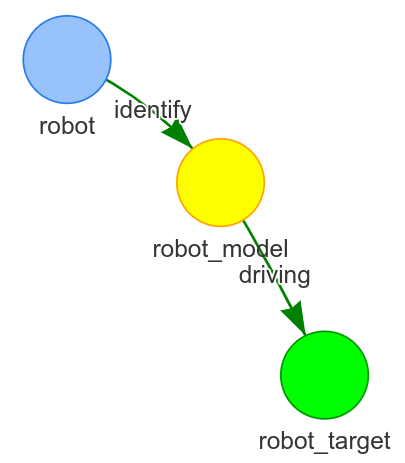
\includegraphics[width=0.8\textwidth]{figures/connecting_nodes/robot_to_target/execute_robot_to_target_3}
    \end{subfigure}
    \caption{Executing the hypothesis found in \cref{fig:robot_drive_hgraph}.}
    \label{fig:execute_robot_to_target}
\end{figure}

Upcoming figure will display the hypothesis generated to push an object to a target position. Both generating a hypothesis and executing the hypothesis are intertwined, this is because certain information should first be collected from the environment before the full hypothesis can be generated. An example is the \textit{best\_push\_position} that can be found in \cref{subfig:robot_push_7,subfig:robot_push_8,subfig:robot_push_9}. The \textit{best\_push\_position} can be found after manipulation planning for the pushing edge is completed. For motion planning a system model is required, thus the corresponding system identification edge should be completed before manipulation planning can start, and than the \textit{best\_push\_position} can be determined.\bs

\begin{figure}[H]
    \centering
    \begin{subfigure}{.3\textwidth}
    \centering
    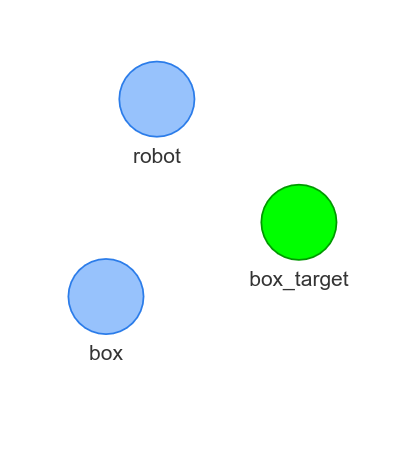
\includegraphics[width=0.8\textwidth]{figures/connecting_nodes/robot_push/robot_push_1}
    \caption{}
    \end{subfigure}
    \begin{subfigure}{.3\textwidth}
    \centering
    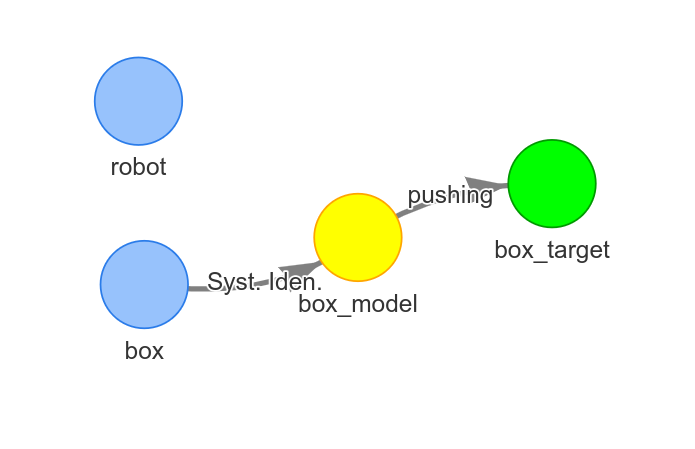
\includegraphics[width=1.1\textwidth]{figures/connecting_nodes/robot_push/robot_push_2}
    \caption{}\label{subfig:robot_push_2}
    \end{subfigure}
    \begin{subfigure}{.3\textwidth}
    \centering
    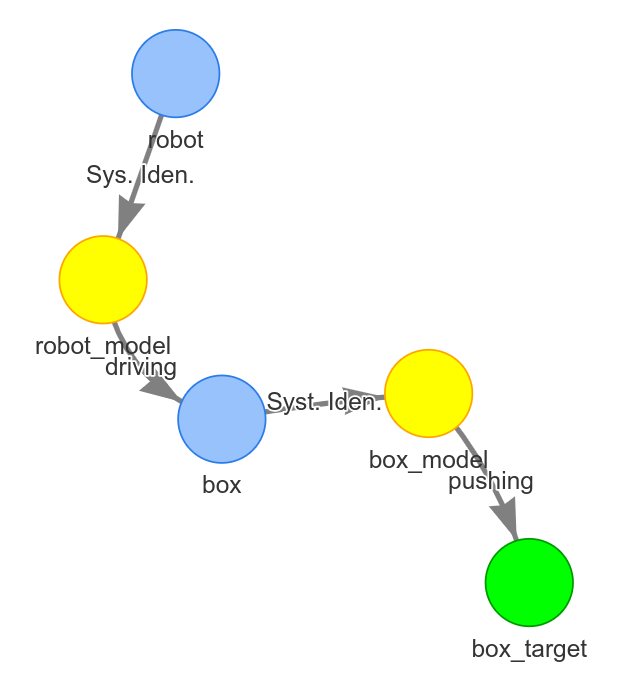
\includegraphics[width=1\textwidth]{figures/connecting_nodes/robot_push/robot_push_3}
    \caption{}\label{subfig:robot_push_3}
    \end{subfigure}

    \begin{subfigure}{.3\textwidth}
    \centering
    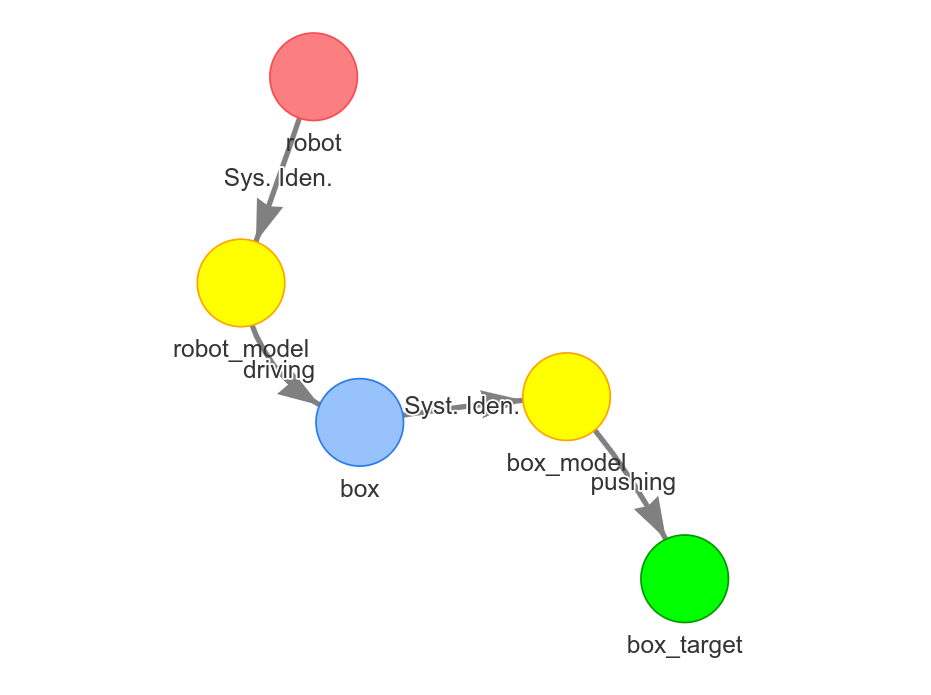
\includegraphics[width=1\textwidth]{figures/connecting_nodes/robot_push/robot_push_4}
    \caption{}\label{subfig:robot_push_4}
    \end{subfigure}
    \begin{subfigure}{.3\textwidth}
    \centering
    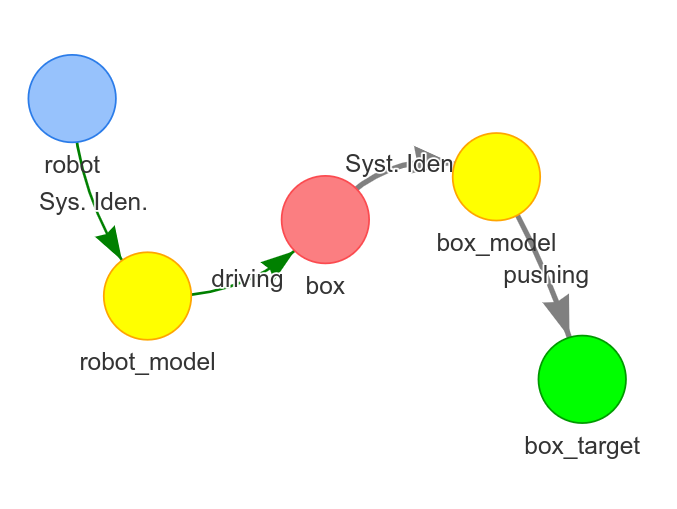
\includegraphics[width=1.05\textwidth]{figures/connecting_nodes/robot_push/robot_push_5}
    \caption{}\label{subfig:robot_push_5}
    \end{subfigure}
    \begin{subfigure}{.3\textwidth}
    \centering
    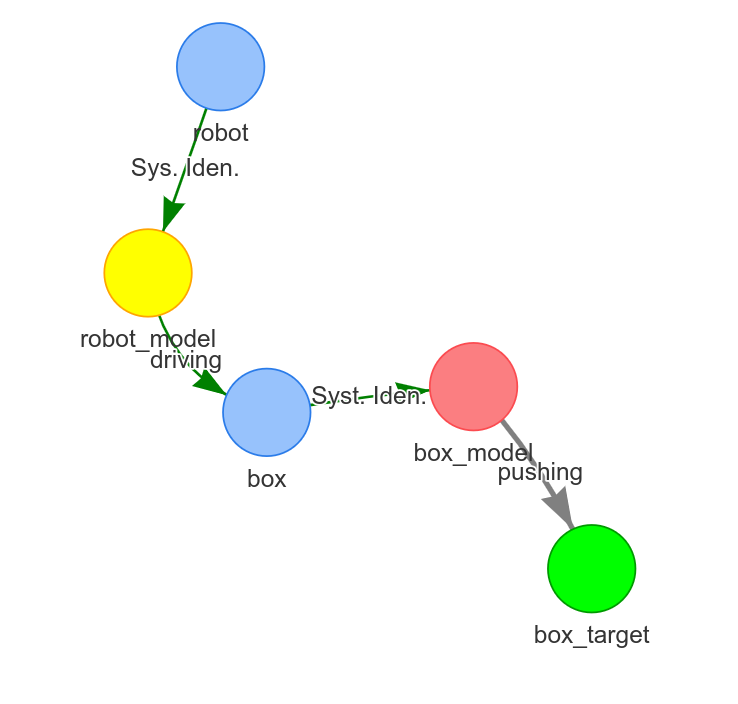
\includegraphics[width=1.05\textwidth]{figures/connecting_nodes/robot_push/robot_push_6}
    \caption{}\label{subfig:robot_push_6}
    \end{subfigure}

    \begin{subfigure}{.3\textwidth}
    \centering
    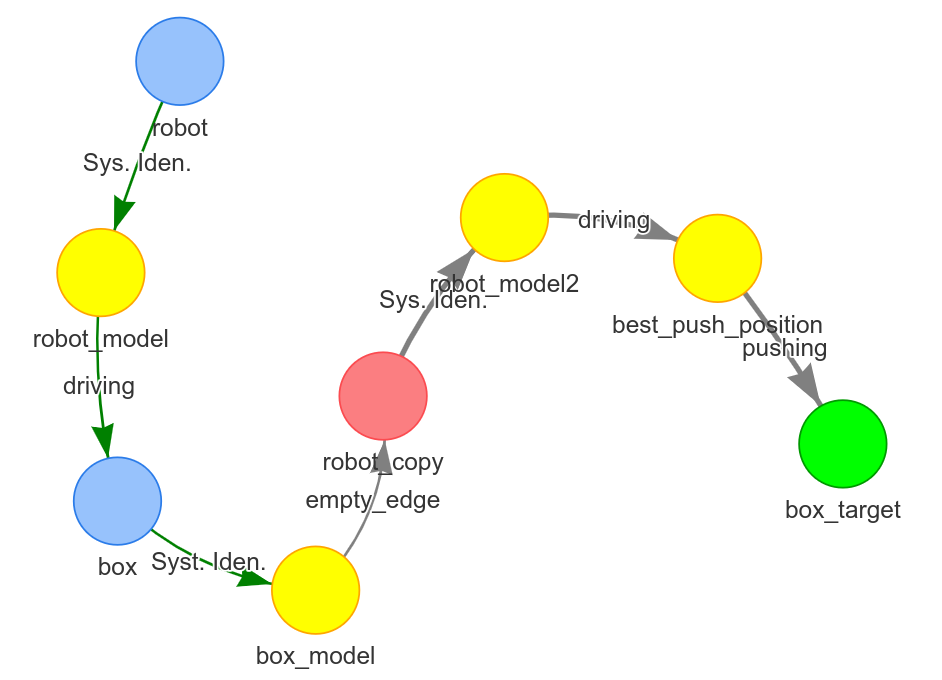
\includegraphics[width=1\textwidth]{figures/connecting_nodes/robot_push/robot_push_7}
    \caption{}\label{subfig:robot_push_7}
    \end{subfigure}
    \begin{subfigure}{.3\textwidth}
    \centering
    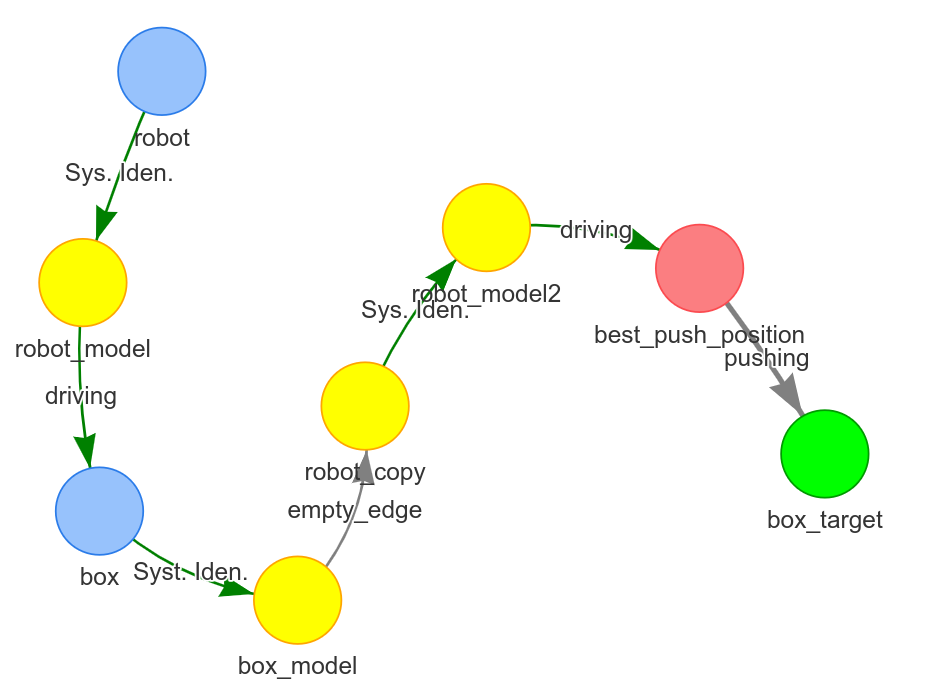
\includegraphics[width=1.05\textwidth]{figures/connecting_nodes/robot_push/robot_push_8}
    \caption{}\label{subfig:robot_push_8}
    \end{subfigure}
    \begin{subfigure}{.3\textwidth}
    \centering
    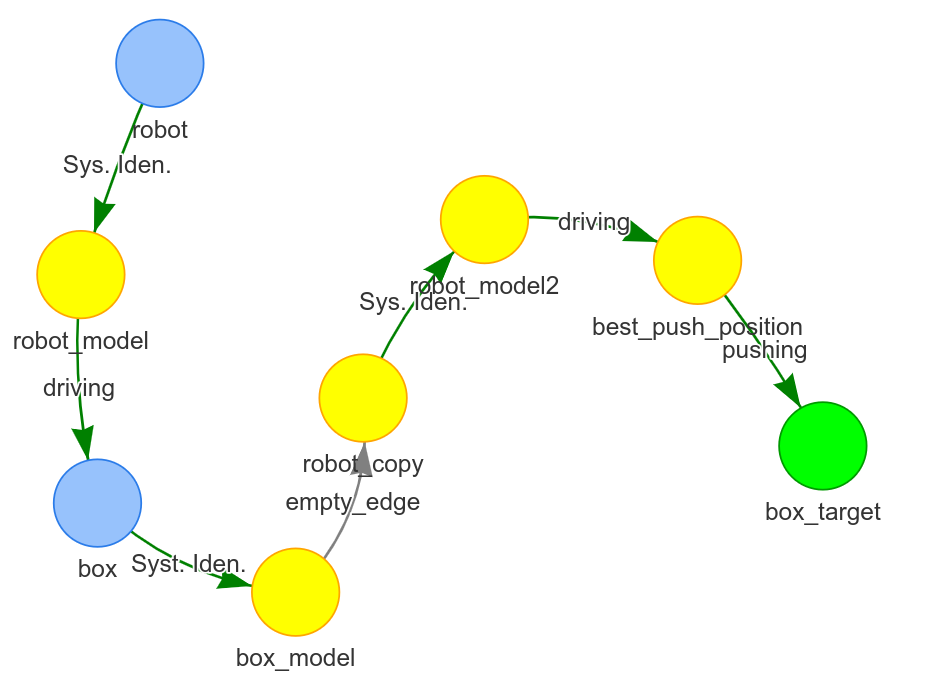
\includegraphics[width=1.05\textwidth]{figures/connecting_nodes/robot_push/robot_push_9}
    \caption{}\label{subfig:robot_push_9}
    \end{subfigure}
    \caption{\ac{hgraph} for pushing the green box to the target configuration}%
    \label{fig:robot_push_hgraph}
\end{figure}
Especially in \cref{subfig:robot_push_2,subfig:robot_push_3} the backward search is clearly visible, the \ac{halgorithm} searches from target node to the robot node. \Cref{fig:robot_push_hgraph} is extensive because every nessecary steps is included whilst some could be skipped. First, identifying a system model for robot driving twice, if the system model created in edge Sys. Iden. pointing toward node robot\_model is reused, then the edge Sys. Iden. pointing toward robot\_model\_1 would be unnecessary. Second, if system models would already be availeble for driving and pushing, no single system identification edge would be required. A \textit{empty\_edge} can be seen in \cref{subfig:robot_push_7,subfig:robot_push_8,subfig:robot_push_9}, the empty\_edge serves to connect a node to another node (box\_model to robot\_copy in \cref{fig:robot_push_hgraph}). The empty\_edge can be traversed without execution, holds no controller, system model or status.\bs

\paragraph{Encountering a Blocked Path}%
During propagation of an action edge's status, motion or manipulation planning occurs. If an object is blocking the path, planning will detect it and the \ac{halgorithm} tries to free the path. In the next example the \ac{halgorithm} detects a blocking object and frees the path by pushing the blocking object to a new configuration, and can be visulised in \cref{fig:blocking_obj_hgraph}.\bs

\begin{figure}[H]
    \centering
    \begin{subfigure}{.3\textwidth}
    \centering
    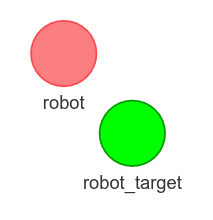
\includegraphics[width=0.5\textwidth]{figures/connecting_nodes/blocking_obj/blocking_obj_1}
    \caption{}
    \end{subfigure}
    \begin{subfigure}{.3\textwidth}
    \centering
    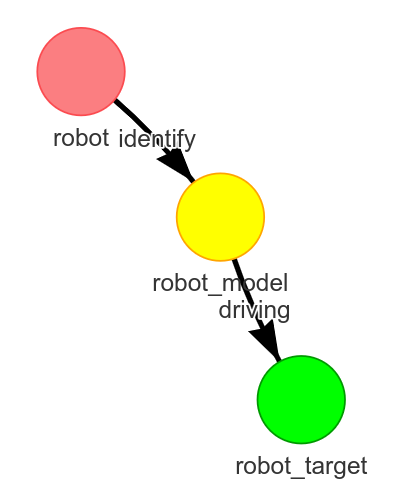
\includegraphics[width=\textwidth]{figures/connecting_nodes/blocking_obj/blocking_obj_2}
    \caption{}\label{subfig:blocking_obj_2}
    \end{subfigure}
    \begin{subfigure}{.3\textwidth}
    \centering
    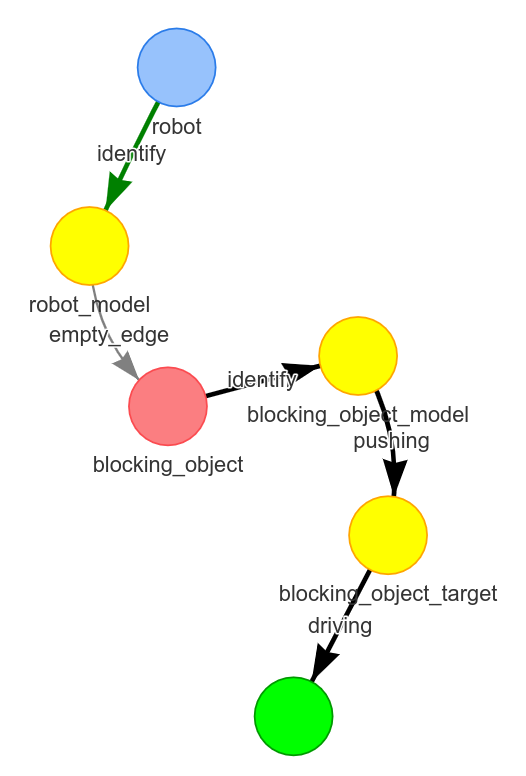
\includegraphics[width=\textwidth]{figures/connecting_nodes/blocking_obj/blocking_obj_3}
    \caption{}\label{subfig:blocking_obj_3}
    \end{subfigure}

    \begin{subfigure}{.3\textwidth}
    \centering
    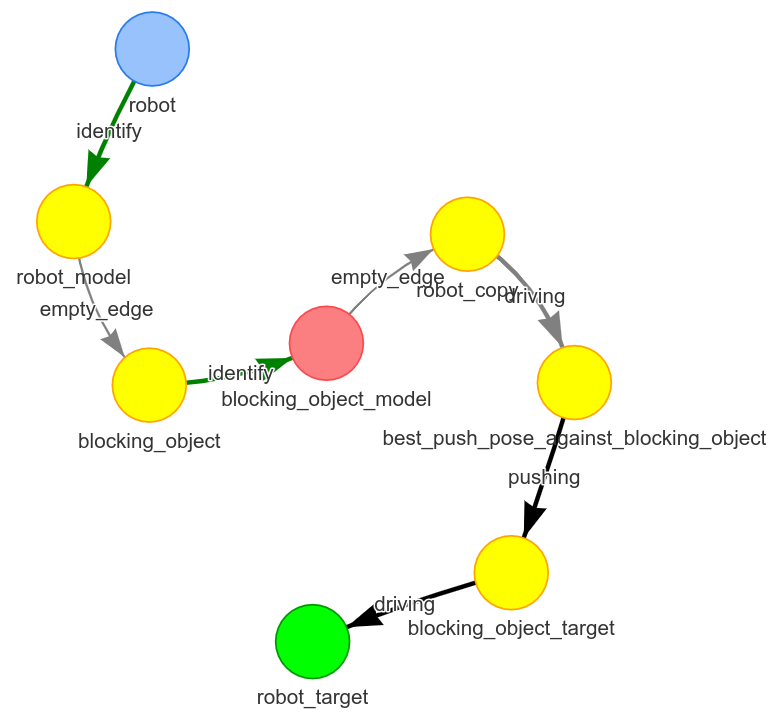
\includegraphics[width=1.3\textwidth]{figures/connecting_nodes/blocking_obj/blocking_obj_4}
    \caption{}\label{subfig:blocking_obj_4}
    \end{subfigure}
    \begin{subfigure}{.3\textwidth}
    \centering
    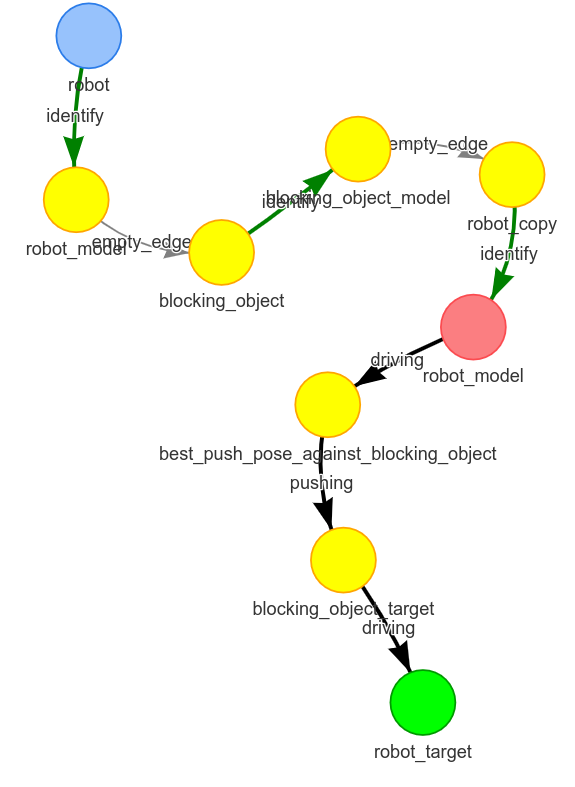
\includegraphics[width=\textwidth]{figures/connecting_nodes/blocking_obj/blocking_obj_5}
    \caption{}\label{subfig:blocking_obj_5}
    \end{subfigure}
    \begin{subfigure}{.3\textwidth}
    \centering
    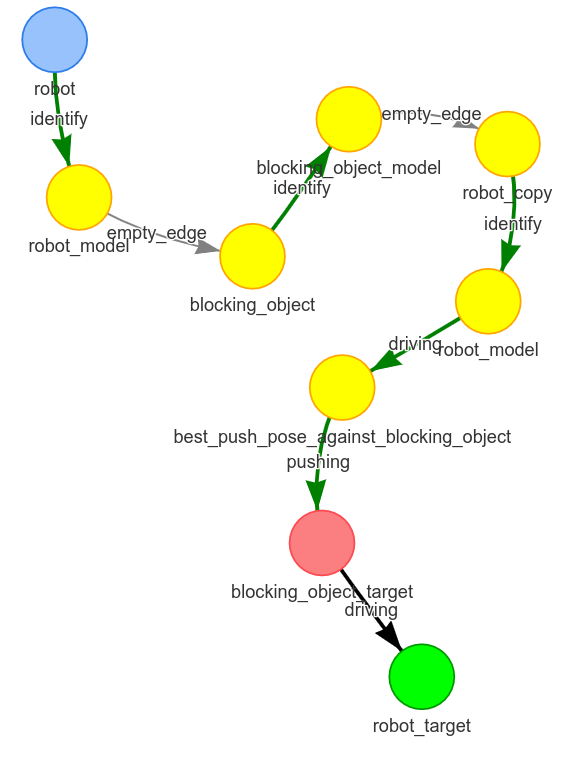
\includegraphics[width=\textwidth]{figures/connecting_nodes/blocking_obj/blocking_obj_6}
    \caption{}\label{subfig:blocking_obj_6}
    \end{subfigure}
    \caption{\ac{hgraph} for driving to target configuration and encountering a blocked path}%
    \label{fig:blocking_obj_hgraph}
\end{figure}

\paragraph{Encountering Failure}%
In the last example, the first hypothesis fails to complete and the \ac{halgorithm} tries to generate a new hypothesis that also fails to complete. Several faults and failures are modelled, the \ac{halgorithm} response to faults and failure is the same. If during the propagation of an edge's status any kind of failure arises, the failed edge and corresponding edges are marked as failed. Equally during execution, if a fault is detected, the execution halts and the edge and corresponding edges are marked as \quotes{failed}, the procedure can be seen in \cref{fig:failure_in_hgraph}.\bs

\begin{figure}[H]
    \centering
    \begin{subfigure}{.3\textwidth}
    \centering
    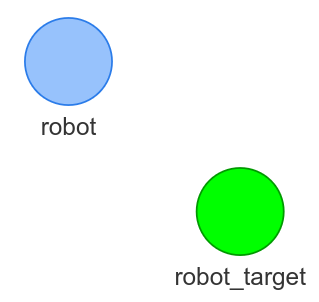
\includegraphics[width=0.8\textwidth]{figures/connecting_nodes/failure/fail_1}
    \end{subfigure}
    \begin{subfigure}{.3\textwidth}
    \centering
    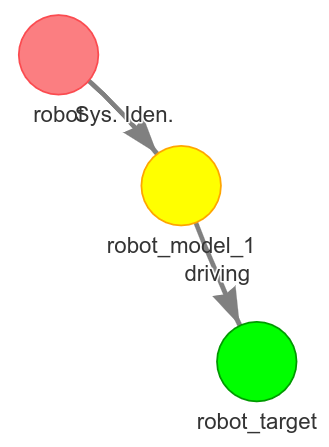
\includegraphics[width=1.1\textwidth]{figures/connecting_nodes/failure/fail_2}
    \end{subfigure}
    \begin{subfigure}{.3\textwidth}
    \centering
    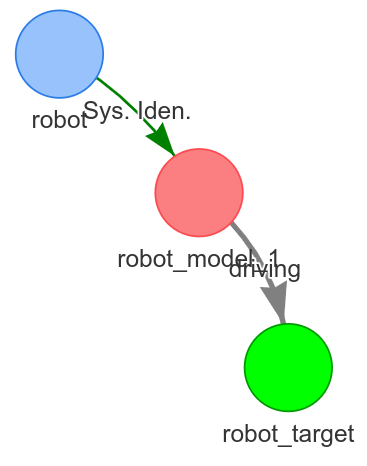
\includegraphics[width=1\textwidth]{figures/connecting_nodes/failure/fail_3}
    \end{subfigure}

    \begin{subfigure}{.3\textwidth}
    \centering
    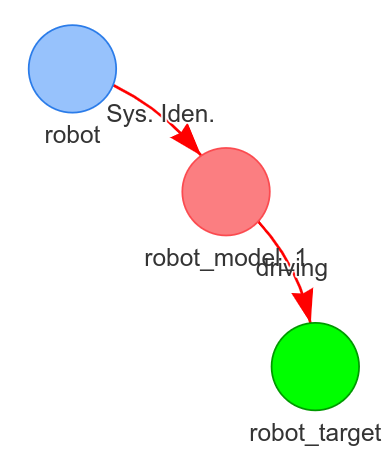
\includegraphics[width=1\textwidth]{figures/connecting_nodes/failure/fail_4}
    \end{subfigure}
    \begin{subfigure}{.3\textwidth}
    \centering
    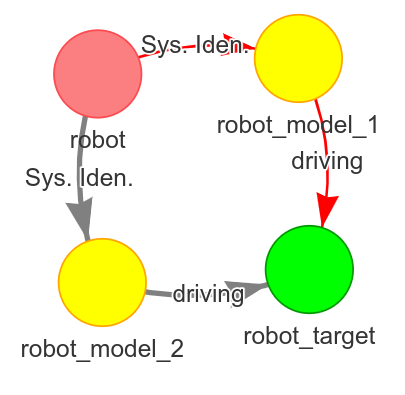
\includegraphics[width=1\textwidth]{figures/connecting_nodes/failure/fail_5}
    \end{subfigure}
    \begin{subfigure}{.3\textwidth}
    \centering
    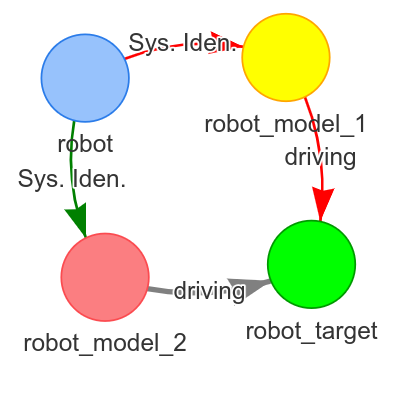
\includegraphics[width=1\textwidth]{figures/connecting_nodes/failure/fail_6}
    \end{subfigure}

    \begin{subfigure}{.3\textwidth}
    \centering
    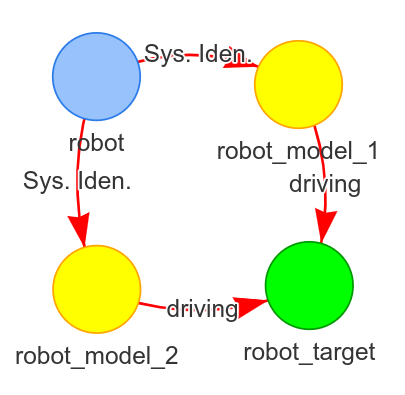
\includegraphics[width=1\textwidth]{figures/connecting_nodes/failure/fail_7}
    \end{subfigure}
    \hfill
    \caption{Executing two hypothesis, both failing to complete because a fault of failure emerged.}%
    \label{fig:failure_in_hgraph}
\end{figure}

In \cref{fig:failure_in_hgraph} only two parameterisations of drive controller and system model were available. Thus after two failed hypothesis the \ac{halgorithm} concludes it cannot complete this task.\bs


What by now hopefully became clear to the reader is that the \ac{hgraph} autonomously searches for hypotheses to solve the task, one subtask at a time. The \ac{hgraph} switches between the search and execution loop. Switching from the search loop toward the execution loop when a hypothesis is found, and switching back when a hypothesis is completed or an action failed to complete.\bs

The limited number of possible edges (every combination of a system identification method with a compatible control method) guarantees that the robot tries to connect 2 nodes, but concludes that it cannot reach a node if all possible edges have failed. Eventually running out of nodes to connect and conclude that a subtask cannot be completed.\bs

In the next section, the edges that are executed will be reviewed and stored in a knowledge base. The knowledge base will suggest edges when faced with similar nodes to connect.
\

\section{Hypothesis Algorithm}%
\label{sec:h-algorithm}
The \ac{h-algorithm} is the main component that orchestrates the actions and functions called to learn object properties and to complete a given task. This section starts with a simple example that generates and executes the hypothesis to drive toward a target pose. Then the search and execution loop are presented, that constitute the principal components of the proposed \ac{h-algorithm}. The terminology is elaborated upon step wise, whilst an example of a pushing task is discussed. Then two more examples are provided that allow to elaborate upon fault detection, the blocklist and the \ac{h-algorithm}'s response to a blocked path during task execution. Finally, the pseudocode can be resented, supported by a proposed \ac{h-algorithm} flowchart.\bs

Two arguments initialize the \ac{h-algorithm}, first, a set of object geometry that contains the dimensions of the objects in the robot environment for internal representation, and second a task to solve. Additionally several parameters must be specified, such as the grid size, maximum allowed input to the robot and tuning parameters for the path estimator, the path planner and controllers. When all arguments and parameters are provided, the \ac{h-algorithm} can be is initialized. There is only a single access point toward the \ac{h-algorithm}, the \textit{Respond(observation)} function. This function takes an environment \textit{observation} that updates the internal objects' poses. The function \textit{Respond($\cdot$)} returns control input for the robot. In this thesis, the sensor measurements coincide with the poses objects in the environment. Recall that the perfect-sensor assumption, assumption~\ref{assumption:perfect_object_sensor}, makes access to every object's exact configuration possible.\bs

Now a relatively simple example is presented to indicate how the \ac{h-algorithm} operates, later every step will be extensively elaborated. The example task consists of driving the robot object to a target pose. The leftmost subfigure in \cref{fig:robot_drive_h-graph} visualizes the initialization of a start and target node, which are connected with a drive action edge in the center figure. In the center subfigure, a system model must be provided to the controller that resides in the drive action edge. Motivating the \textit{sys. iden} edge and the $\gls{c}_\textit{robot\_model}$ node in the rightmost subfigure.\bs

\begin{figure}[h]
    \centering
    \begin{subfigure}{.3\textwidth}
    \centering
    \includegraphics[width=0.7\textwidth]{figures/proposed_method/connecting_nodes/robot_to_target/robot_to_target}
    \end{subfigure}
    \begin{subfigure}{.3\textwidth}
    \centering
    \includegraphics[width=0.9\textwidth]{figures/proposed_method/connecting_nodes/robot_to_target/robot_drive_target}
    \end{subfigure}
    \begin{subfigure}{.3\textwidth}
    \centering
    \includegraphics[width=\textwidth]{figures/proposed_method/connecting_nodes/robot_to_target/robot_iden_drive_target}
    \end{subfigure}
    \caption{First stages of the \ac{h-graph} when the \ac{h-algorithm} searches for an hypothesis to complete a driving task.}%
    \label{fig:robot_drive_h-graph}
\end{figure}

Now that an hypothesis is created that consists of an identification- and an action edge, the \ac{h-algorithm} alternates from the search loop to the execution loop, both loops are addressed shortly. The generated and executed example for a driving task just discussed is provided to show a simple example. It leaves many details out, which are now elaborated. Start with initializing start- and target nodes, then the search- and execution loop are discussed.\bs

\paragraph{Initialization of the \ac{h-algorithm}}
The \ac{h-algorithm} is initialized with a task that consists of one or more subtasks. Start- and target nodes are created for every subtask, and their status is set to INITIALIZED. Then the goal of the \ac{h-algorithm} is to connect every starting node to its corresponding target node with a hypothesis. The target node's status is set to COMPLETED when a hypothesis is completed successfully. If the \ac{h-algorithm} could not find a hypothesis that completes a subtask, the \ac{h-algorithm} concludes it cannot complete that subtask, and the target node's status is set to FAILED.\bs

\begin{figure}[H]
    \centering
    \begin{subfigure}{.3\textwidth}
    \centering
    \includegraphics[width=0.9\textwidth]{figures/proposed_method/connecting_nodes/robot_to_target/execute_robot_to_target_1}
    \end{subfigure}
    \begin{subfigure}{.3\textwidth}
    \centering
    \includegraphics[width=0.9\textwidth]{figures/proposed_method/connecting_nodes/robot_to_target/execute_robot_to_target_2}
    \end{subfigure}
    \begin{subfigure}{.3\textwidth}
    \centering
    \includegraphics[width=0.9\textwidth]{figures/proposed_method/connecting_nodes/robot_to_target/execute_robot_to_target_3}
    \end{subfigure}
    \caption{Multiple stages of the \ac{h-graph} when the \ac{h-algorithm} executes the hypothesis found in \cref{fig:robot_drive_h-graph}.}
    \label{fig:execute_robot_to_target}
\end{figure}

\subsection{The Search and the Execution Loop}
The proposed algorithm comprises two main parts, a search loop and an execution loop. The \ac{h-algorithm} searches for a hypothesis in the search loop. In the execution loop, the \ac{h-algorithm} tests hypotheses by executing the edges that form the hypothesis. A flowchart  of the \ac{h-algorithm} is presented at the very end of this chapter in \cref{tikz:flowchart_h-algorithm}, that flowchart will be familiar compared to the following figure, where the two main loops can be identified.\bs

\begin{figure}[H]
    \centering
    \includegraphics[width=7cm]{figures/proposed_method/two_loops_identified}
  \caption{The search (upper) and execution (lower) loop, that make up the main part of the proposed \ac{h-algorithm}. The figure's goal is to present the two loops, the flowchart in the background is presented full page in \Cref{tikz:flowchart_h-algorithm}.}%
    \label{fig:two_loops_identified}
\end{figure}

Hypotheses are formed while the \ac{h-algorithm} resides in the search loop. Forming a hypothesis generates nodes, edges, and progressing their status as described in \cref{tikz:status_identification_edge,tikz:status_action_edge}. In the execution loop \textit{an edge is being executed}, a phrase to describe that the controller residing in an edge is sending control input toward the robot. The \ac{h-algorithm} operates synchronously. The result is that the robots cannot operate whilst the \ac{h-algorithm} resides in the search loop, and during execution, no hypothesis can be formed or updated. The execution loop executes the edges that form the hypothesis one by one until either a fault is detected or the hypothesis is completed. Upon fault or completion, the \ac{h-algorithm} alternates back to the search loop\bs

When entering or re-entering the search loop, the first thing to determine is if there are unfinished subtasks and, if unfinished subtasks exist, which nodes to connect in order to form a hypothesis that completes that subtask. For such functionality three functions are created; \textit{SubtaskNotFinished}, \textit{GoBackward(\gls{node})}, \textit{FindCorrespondingNode(\gls{node})}. These functions are now discussed.\bs

\paragraph{Finding unfinished subtasks}
Determining if there exists an unfinished subtask is validated with the \textit{SubtaskNotFinished(\gls{task})} function. It checks the status for every target node in \ac{h-graph}. The three statuses are; INITIALIZED, COMPLETED and FAILED. A target node with an INITIALIZED status corresponds to an uncompleted subtask and is returned by the \textit{SubtaskNotFinished(\gls{task})} function. If all existing target nodes have either a completed or failed status, the \ac{h-algorithm} concludes that the task is completed.\bs

The \ac{h-algorithm} relies on a backward search technique, which can be described as: \textit{start the search at a goal state and work backwards until the initial state is encountered~\cite{lavalle_planning_2006}.} A motivation for a backward search over a forward search is that it might be the case that the branching factor is significant when starting from the initial state. In such cases, it might be more efficient to use a backward search. If the \textit{SubtaskNotFinished} returns an unfinished subtask, the \ac{h-algorithm} starts searching for a hypothesis connecting the start node to the corresponding target node. The first step is to find the right nodes in the \ac{h-graph}, which is now discussed.\bs

\paragraph{Creating a hypothesis for a subtask}
The \textit{SubtaskNotFinished} returns a target node corresponding to a unfinished subtask. Then if a subtask is unfinished, the \ac{h-algorithm} starts searching for a hypothesis connecting the start node to the target node. In \cref{subfig:robot_push_1}, the nodes to connect are the $\gls{node}_\mathit{box}$ node to the $\gls{node}_\textit{box\_target}$ node. These two nodes are a start- and a target node, the nodes to connect are not necessarily start- and target nodes themselves, as seen in \cref{subfig:robot_push_2}. Here the $\gls{node}_\textit{robot}$ node must be connected to the $\gls{node}_\textit{box}$ node. These nodes are both starting nodes. The first challenge is to find the two nodes to connect from an unfinished target node.\bs

The \textit{GoBackward($\gls{node}_\mathit{target}$)} function takes a target node $\gls{node}_\mathit{target}$ that corresponds to a unfinished subtask. It then traverses backwards via non-failed edges. The function stops traversing back when it encounters a node with a FAILED status or when no non-failed edge exists to traverse backwards over. The \textit{GoBackward} function thus finds a node, that node points toward the target node over a sequence of edges with a status other than failed, and all these edges point toward nodes with a status other than failed. In \cref{subfig:robot_push_1} the \textit{GoBackward($\gls{node}_\mathit{box\_target})$} function returns the $\gls{node}_\mathit{box\_target}$ node, in \cref{subfig:robot_push_2} the \textit{GoBackward($\gls{node}_\mathit{box\_target})$} returns the $\gls{node}_\mathit{box}$ node.\bs

The \textit{GoBackward($\gls{node}_\mathit{target}$)} finds a node to connect to, a corresponding node is sought to connect from. The \textit{FindCorrespondingNode(\gls{node})} finds a corresponding node to connect from. \textit{FindCorrespondingNode(GoBackward(\gls{node}))} takes a node as parameter and returns an existing node that contains the same object as its arguments node; if such a node does not exist, a new node is created.
\[\gls{node}_\mathit{to} =  \mathit{GoBackward(\gls{node}_\mathit{target})}\]
\[\gls{node}_\mathit{from} = \mathit{FindCorrespondingNode(GoBackward(\gls{node}_\mathit{target}))}\]

When elaborating the \ac{h-algorithm}, an example presents a visual example with every step in the \ac{h-algorithm}. In this example, the robot generates a hypothesis to complete a pushing task that contains a single subtask, initialization and the first generated edges are presented in \cref{fig:robot_push_1}.\bs

\begin{figure}[h]
    \centering
    \begin{subfigure}{.3\textwidth}
    \centering
    \includegraphics[width=0.9\textwidth]{figures/proposed_method/connecting_nodes/robot_push/robot_push_1}
    \caption{Initialize start- and target nodes.}\label{subfig:robot_push_1}
    \end{subfigure}
    \begin{subfigure}{.32\textwidth}
    \centering
    \includegraphics[width=\textwidth]{figures/proposed_method/connecting_nodes/robot_push/robot_push_2_new}
    \caption{Creation of a push action edge.}\label{subfig:robot_push_2}
    \end{subfigure}
    \begin{subfigure}{.35\textwidth}
    \includegraphics[width=1.2\textwidth]{figures/proposed_method/connecting_nodes/robot_push/robot_push_2}
    \caption{Creation of a identification edge.}\label{subfig:robot_push_3}
    \end{subfigure}
    \caption{First stages of the \ac{h-graph} when the \ac{h-algorithm} creates an hypothesis for a pushing task.}%
    \label{fig:robot_push_1}
\end{figure}

\paragraph{Creating edges}
The \textit{ConnectWithEdge($\gls{node}_1, \gls{node}_2$)} function connects two nodes with an edge, such as the nodes $\gls{node}_\mathit{from}, \gls{node}_\mathit{to}$ just introduced. It is required that both nodes contain the same object. The push action edge generated and displayed in \cref{subfig:robot_push_2} is between two nodes containing the \textit{box} object.\bs

Pushing edges must satisfy pre-conditions that cannot reside in the pushing edge itself. Thus pushing edges also they spawn new nodes by default. The robot must first drive toward a push pose against or close to the object to push. When a push action edge has planned a path, and updates its status to PATH IS PLANNED, the \ac{h-algorithm} then creates a $\gls{node}_\mathit{best\_push\_position}$ node, which configuration depends on the object's planned path. Thus, a path is planned for the push action, and then the best push pose is determined. The newly created node is connected before the push action edge, where an empty edge points from $\gls{node}_\mathit{best\_push\_position}$ to $\gls{edge}_\mathit{drive}$'s source node. The first occurrence of an $\gls{node}_\mathit{best\_push\_position}$ can be visualized in \Cref{subfig:robot_push_4}.\bs

\paragraph{Classifying objects}
When it is unknown if objects are movable or unmovable, a push action edge performs a tests to determine the class of an object. If the push action is unable to move the object in the first 50 time steps, the object is classified as UNMOVABLE, otherwise it is classified as MOVABLE.\bs

\paragraph{Valid Hypotheses}
Before a hypothesis can be executed, the hypothesis must be valid. A hypothesis is valid when two conditions are met. First, the hypothesis starts at the start node and points toward the target node over a sequence of successive edges with a non-failing status. Second, the first edge in the hypothesis must be ready for execution which the next paragraph will elaborate upon further. To indicate a node or edge has a status other than the FAILED status, that node or edge is called a non-failed node or -edge. To check if an hypothesis is valid the \textit{IsConnected($\gls{node}_1, \gls{node}_2$)} is created. This function checks if there exists a path in the \ac{h-graph} from $\gls{node}_1$ to $\gls{node}_2$ over a sequence of non-failing nodes and -edges. In the pushing task example, the first occurrence of a valid hypothesis is presented in \Cref{subfig:robot_push_4}.\bs

An \textit{EmtpyEdge} is introduced to involve nodes that contain different objects. The emptyEdge serves only to connect nodes that contain different objects and can have status INITIALIZED or FAILED. The \ac{h-algorithm} can traverse over emptyEdge if the status is INITIALIZED.\bs

\begin{figure}[H]
    \centering
    \begin{subfigure}{.45\textwidth}
    \centering
    \includegraphics[width=1\textwidth]{figures/proposed_method/connecting_nodes/robot_push/robot_push_4_new}
    \caption{Executing the hypothesis and generated new nodes.}\label{subfig:robot_push_4}
    \end{subfigure}
    \begin{subfigure}{.45\textwidth}
    \centering
    \includegraphics[width=1\textwidth]{figures/proposed_method/connecting_nodes/robot_push/robot_push_5_new}
    \caption{Executing the pushing edge.}\label{subfig:robot_push_5}
    \end{subfigure}
    \caption{The hypothesis for a pushing task becomes valid and is executed. Then a path for the pushing edge\\is planned which generates new nodes to drive toward the best push pose against the box.}%
    \label{fig:robot_push_2}
\end{figure}

\paragraph{Preparing edges for Execution}
In contrast to identification edges, action edges must first take several actions in preparation before they are ready to send input toward the robot. The status of an edge indicates at which step of preparing the action edge is and can be visualized in \Cref{tikz:status_action_edge}. After initialization, the action edge performs path estimation, loads in a system model, performs path planning and then, it is ready for execution. Two functions are created to make edges ready for execution. The \textit{ReadyForExecution(\gls{edge})} validates if an edge is ready for execution. Identification edges are ready for execution when they bear a non-failed status, action edges are ready for execution when they bear the PATH PLANNED or EXECUTING status. The \textit{MakeReady(\gls{edge})} function takes an edge and takes action depending on its status presented in the following table.\bs

\begin{table}[H]
    \caption{The action edge status is presented in the left column, the corresponding action taken by the \textit{MakeReady} function to prepare an action edge for execution in the right column. An action edge increments its status as indicated in \Cref{tikz:status_action_edge}.}%
    \label{table:make_action_edge_ready}
    \centering
    \begin{tabular}%
    {>{\raggedright\arraybackslash}p{0.25\textwidth}|%
    >{\raggedright\arraybackslash}p{0.65\textwidth}}
      Action edge status& action taken by \textit{MakeReady} function\\\toprule
      INITIALIZED& Create a path estimator and estimate path existence. If no path can be estimated, the status is updated to FAILED. If a path can be estimated, a shortest path is found that acts as a \quotes{warm start} for the path planner.\\
      PATH EXISTS& Load in a system model.\\
      SYSTEM MODEL& Create path planner and plan path. The edge status is updated to FAILED if no path can be found. If a path is found, it acts as a reference signal for the controller. In the case of an push action edge, a $\gls{node}_\mathit{best\_push\_position}$ is created. Additionally, the path the planner finds can indicate that an object is blocking. In such cases, the \ac{h-algorithm} must first push that object to free the path. An example of such a case is provided in \Cref{fig:blocking_obj_h-graph_one}.
    \end{tabular}
\end{table}

\paragraph{Hypothesis Execution}
When the \ac{h-algorithm} creates a valid hypothesis, it switches from the search loop to the execution loop. Executing a hypothesis is managed by three functions. The first edge in the hypothesis is ready for execution and thus contains a controller and a path to track. That edge is executed, and its controller sends input toward the robot to track the path. The \textit{SteerTowardTarget(\gls{edge})} calculates the input that steers the robot toward the path. The \textit{TargetNotReached(\gls{edge})} validates if the robot has reached the target, which is the last configuration in the path. A margin is set by which the \textit{TargetNotReached(\gls{edge})} concludes that the robot is close enough to the final target pose. For drive actions, that margin is set to 0.1 meters measured in Euclidean instance between the robot and the robot's target position.

For push action, that margin is set to 2 meters, measured in Euclidean distance between the object and the object's target position. These values are tuned by trial and error and is one of the improvements that can be made in future work. The large margin for pushing tasks is set to ensure that the target pose is reached. With a lower margin, the object is often pushed further than the target position. A fault is then detected because the deviated too much from the path, the robot then drives toward the object's opposite side to again, push it over the target position. Fault detection is discussed in upcoming paragraph. After the successful completion of an edge, the next edge in the hypothesis is selected by the \textit{IncrementEdge} function. Two possible outcomes exist, the next edge is ready for execution, then the \ac{h-algorithm} remains in the execute loop. Or, the next edge is not yet ready, then the \ac{h-algorithm} goes from the execution loop toward the search loop to prepare the next edge for execution.\bs

\begin{figure}[H]
    \centering
    \includegraphics[width=0.5\textwidth]{figures/proposed_method/connecting_nodes/robot_push/robot_push_6}
    \caption{The \ac{h-graph} after the pushing task was successfully completed.}%
    \label{fig:robot_push_5}
\end{figure}

\paragraph{Completing Hypotheses and Edges}
When the last edge in an hypothesis is completed, that subtask is completed. The \ac{h-graph} randomly selects a next subtask to complete until there are no unfinished subtasks left, the \ac{h-algorithm} then concludes that the task is completed. Opposed to successful completion, subtasks can unsuccessfully complete, which is discussed in the upcoming paragraph.\bs

\subsection{Fault Detection}%
\label{sec:monitoring_metrics}
The proposed framework implements a fault metric named the \textit{monitored metrics} which are presented shortly, first motivation for the monitoring metrics is given. When the \ac{h-algorithm} resides in the execution loop, it cannot search for action sequences, which is performed in the search loop. During the execution of an action, the \acl{h-algorithm} is unable to perform any other action. This blocking behavior has some implications, mainly that the controller can steer the system to a configuration from which it cannot independently reach the target configuration, as a result, it will never halt. For example, a controller tries to drive the robot toward a target configuration but there is an unmovable obstacle in the way. Another example is the controller is closed-loop unstable and never reaches its target configuration. Both examples do not occur is well defined simulation environments, because of the \textit{closed-world assumption}. In the real world, an unexpected blocking obstacle or unstable controllers are more likely to occur.\bs

Detecting controller faults is a large robotic topic~\cite{khalastchi_fault_2019}, properly implementing a fault detection and diagnosis module is out of the scope of this thesis. Instead, two simple metrics will be monitored during execution, by the \textit{FaultDetected(\gls{edge})} function. Upon detection of a fault, the \textit{HandleFault(\gls{edge})} function then updates the executing edge's status to FAILED, and the \ac{h-algorithm} switches from the execution loop to the search loop in search for a new hypothesis. The first monitoring metric is \acl{PE}, and can be described as:\\
With the current configuration of the system, calculated system input and a system model, a prediction info the future is made every time step. Then the system input is applied to the system, the time step incremented and the configuration is measured. The prediction error is than the difference between predicted and measured configuration.\bs

The \ac{PE} is defined as:

\[ \gls{pe}(\gls{k}) ::= ||\gls{Cest}(\gls{k}|\gls{k}-1) - \gls{c}(\gls{k})|| \]

Where $\gls{Cest}(\gls{k}|\gls{k}-1)$ is a prediction of the configuration and $\gls{c}(\gls{k})$ is the measured configuration.\bs

During execution a sudden high \ac{PE} indicates unexpected behavior occurs, such as when the robot has driven into an object which it was not expecting. A high \ac{PE}, which persists indicates that the robot is continuously blocked. A few high prediction errors are allowed, but when the \ac{PE} exceeds a pre-defined threshold and persists over a pre-defined time, the \ac{h-graph} concludes that there was an fault detected during execution and the edge's status is updated to FAILED.\bs

The second monitoring metric is the \acl{TE} that can be described as:\\ A controller tracks a path that consists of a list of configurations by steering the system to the upcoming configuration in the list. When that configuration is reached, the upcoming configuration is updated to the next configuration in the path. The \ac{TE} is the difference between the current configuration of the system and the upcoming configuration.\bs

The \ac{TE} is defined as:

\[ \gls{te}(\gls{k}) ::= ||\gls{c}_\mathit{upcoming} - \gls{c}(\gls{k})|| \]

Where $\gls{c}_\mathit{upcoming}$ is the target configuration in the path that the controller tries to steer toward, and \gls{c}(\gls{k}) is the measured configuration.\bs

The system should not diverge too far from to path it is supposed to track, if the robot diverges more than a pre-defined threshold the \ac{h-graph} concludes that there was an error during execution and the edge fails. $\gls{c}_\mathit{upcoming}$ does not update every time step, whilst \gls{c}(\gls{k}) does update every time step. As a result, a \quotes{good} \ac{TE} is expected to take the form of a saw tooth function inverted over the horizontal x-axis.\bs

The predefined thresholds are split for drive and push actions because driving actions have much lower average \ac{PE} and \ac{TE} compared to push actions. For drive action edges, when the average of the last 25 recorded \ac{PE}'s is higher than 0.05 meter, or the \ac{TE} is higher than 2 meters, a fault is concluded. For push actions only a \ac{TE} is used, which is split into two parts. One ensures the object follows the path, and another ensures that the robot does not deviate too far from the object. If, for a pushing edge, the object deviates more than 2 meters from the path or the robot deviates more than 2 meters from its push position determined by the object pose, a fault is concluded.\bs

\subsection{The Blocklist}%
The blocklist prevents the regeneration of failed edges. The infinite loop of creating an edge that fails only to be regenerated is prevented. The blocklist keeps a list of edge parameterization as well as the node identifier if failed on. Newly generated edges are checked against this blocklist, if they are on the blocklist, initialization of the edge is prevented. The possible parameterizations are filtered when two nodes are connected with an action edge. Thus, any parameterization on the blocklist for a specific node (to which the action edge would point to) cannot be created again for the lifetime of the \ac{h-graph}.\bs

In the following example, \Cref{fig:failure_in_h-graph} faults are detected, these edges are added to the blocklist, the first hypothesis fails to complete, and the \ac{h-algorithm} tries to generate a new hypothesis that also fails to complete.\bs

\begin{figure}[H]
    \centering
    \begin{subfigure}{.3\textwidth}
    \centering
    \includegraphics[width=\textwidth]{figures/proposed_method/connecting_nodes/failure/fail_2}
    \end{subfigure}
    \begin{subfigure}{.3\textwidth}
    \centering
    \includegraphics[width=\textwidth]{figures/proposed_method/connecting_nodes/failure/fail_3}
    \end{subfigure}
    \begin{subfigure}{.3\textwidth}
    \centering
    \includegraphics[width=\textwidth]{figures/proposed_method/connecting_nodes/failure/fail_4}
    \end{subfigure}

    \begin{subfigure}{.3\textwidth}
    \centering
    \includegraphics[width=1\textwidth]{figures/proposed_method/connecting_nodes/failure/fail_5}
    \end{subfigure}
    \begin{subfigure}{.3\textwidth}
    \centering
    \includegraphics[width=1\textwidth]{figures/proposed_method/connecting_nodes/failure/fail_6}
    \end{subfigure}
    \begin{subfigure}{.3\textwidth}
    \centering
    \includegraphics[width=1\textwidth]{figures/proposed_method/connecting_nodes/failure/fail_7}
    \end{subfigure}
    \hfill
    \caption{Multiple stages of the \ac{h-graph}. The two hypotheses both failed during execution because a fault was detected. The failed edges are added to the blocklist, preventing the regeneration of edges with the same parameterization. The \ac{h-algorithm} concludes the task to be unfeasible.}%
    \label{fig:failure_in_h-graph}
\end{figure}

In \Cref{fig:failure_in_h-graph}, only two parameterizations of drive controllers and system models were available. Thus after two failed hypotheses, the \ac{h-algorithm} concludes that the task is unfeasible. All functionality is now discussed and is neatly summarized in the following table. Then, pseudocode for the proposed \ac{h-algorithm} is presented.\bs

\subsection{Encountering a Blocked Path}%
During the propagation of an action edge's status, path planning occurs discussed in \Cref{subsec:path_planning,chap:proposed_planning}. A blocking object is detected when the path found crosses through unknown of movable space. An example is now discussed that elaborates upon the \ac{h-algorithm} response when encountering a blocked path. An example of such an environment can be visualized in \Cref{subfig:push_or_drive_env} where the \textit{UnknownSpaceCost} is set to 0.5 meter. The example \ac{h-graph} that will now be discussed generalizes over drive tasks that can be completed if an blocking object is pushed to free the path.\bs

The \ac{h-algorithm} creates the start- and target node for the robot in \Cref{subfig:blocking_obj_1}, and creates a first hypothesis which can be visualized in \Cref{subfig:blocking_obj_2}. When propagating the drive action edge status, path planning occurs, during which a blocking object is detected that blocks a direct path. To free that path two nodes are generated, first, a target node for the blocking object \textit{blocking\_object\_target} that target node indicates the blocking object at a pose that is no longer blocking the path. The second node represents the blocking object at its current pose, because there does not yet exist a node for the blocking object at its current pose, the \ac{h-algorithm} generates a new node for the blocking object at it's current pose named \textit{blocking\_object} that can be seen in \Cref{subfig:blocking_obj_3}.\bs

\begin{figure}[H]
  \centering
  \begin{subfigure}{.3\textwidth}
    \centering
    \includegraphics[width=0.6\textwidth]{figures/proposed_method/connecting_nodes/blocking_obj/blocking_obj_1}
    \caption{}\label{subfig:blocking_obj_1}
  \end{subfigure}
  \begin{subfigure}{.3\textwidth}
    \centering
    \includegraphics[width=0.9\textwidth]{figures/proposed_method/connecting_nodes/blocking_obj/blocking_obj_2}
    \caption{}\label{subfig:blocking_obj_2}
  \end{subfigure}
  \begin{subfigure}{.3\textwidth}
    \centering
    \includegraphics[width=\textwidth]{figures/proposed_method/connecting_nodes/blocking_obj/blocking_obj_3}
    \caption{}\label{subfig:blocking_obj_3}
  \end{subfigure}

  \caption{Multiple stages of the \ac{h-graph} for a driving task, where an blocked path is encountered.}%
  \label{fig:blocking_obj_h-graph_one}

\end{figure}

The newly generated pushing edge between node \textit{blocking\_object\_model} and \textit{blocking\_object\_target} is initialized with a randomly selected controller. To fully parameterize the pushing edge a controller with a compatible system model is required. To generate a system model, the \ac{h-algorithm} generates a pushing identification edge and node \textit{blocking\_object\_model}.\bs

After identifying a system model that describes pushing against the blocking object, path planning for the blocked object from its current pose toward it's target pose occurs. The initial pose for the robot against the blocked object can then be determined because that initial pose is dependent on the planned path. \Cref{subfig:blocking_obj_4} displays the drive edge toward the best initial push pose indicated by the \textit{best\_push\_pose\_against\_blocking\_object} node. Equivalent to the generation of a blocking object node at its current pose in \Cref{subfig:robot_push_3}, a robot node is generated at the current robot's pose, named \textit{robot\_copy} in \Cref{subfig:blocking_obj_4}, because a node at the current robot pose did not yet exist. A drive edge is generated between the \textit{robot\_copy} and \textit{best\_push\_pose\_against\_blocking\_object} nodes. The identification edge is later generated as can be seen in \Cref{subfig:blocking_obj_5}.\bs

\begin{figure}[H]
    \centering
    \includegraphics[width=0.5\textwidth]{figures/proposed_method/connecting_nodes/blocking_obj/blocking_obj_4}
    \caption{Snapshot of the \ac{h-graph} during drive task, where a blocked path is encountered. The (red) current node indicates that next action is to drive toward the best push pose against the blocking object.}\label{subfig:blocking_obj_4}
\end{figure}

\Cref{subfig:blocking_obj_5,subfig:blocking_obj_6} visualize driving toward the best push pose against the blocking object, pushing the blocked object to its target pose, and finally driving toward the robots target pose.\bs

\begin{figure}[H]
  \centering
  \begin{subfigure}{.3\textwidth}
    \centering
  \includegraphics[width=\textwidth]{figures/proposed_method/connecting_nodes/blocking_obj/blocking_obj_5}
    \caption{}\label{subfig:blocking_obj_5}
  \end{subfigure}
  \begin{subfigure}{.3\textwidth}
    \centering
    \includegraphics[width=\textwidth]{figures/proposed_method/connecting_nodes/blocking_obj/blocking_obj_6}
    \caption{}\label{subfig:blocking_obj_6}
  \end{subfigure}
  \caption{\ac{h-graph} final stages before successfully completing a driving task, during which a blocked path is encountered.}%
  \label{fig:blocking_obj_h-graph_two}
\end{figure}

Now that the \ac{h-algorithm} is defined and discussed, pseudocode is presented. The following table summarizes the functions that will be used by the pseudocode in \Cref{pseudocode:h-algorithm}.\bs

\begin{table}[H]
\caption{The functions employed by the \ac{h-algorithm} in \Cref{pseudocode:h-algorithm}.}
\label{table:functions_for_h-algorithm}
\centering
\begin{tabular}%
  {>{\raggedright\arraybackslash}p{0.25\textwidth}%
   >{\raggedright\arraybackslash}p{0.65\textwidth}}
\textit{SubTaskNotFinished(\gls{subtask})}:& Return False if the subtask \gls{subtask} is completed or it is concluded to be unfeasible \\
\textit{IsConnected($\gls{node}_1, \gls{node}_2$)}:& Return True if there exist a path in the \ac{h-graph} from node $\gls{node}_1$  to node $\gls{node}_2$ through a number of non-failed edges\\
\textit{ReadyForExecution(\gls{edge})}: & Return True if the edge \gls{edge} is ready to execute\\
\textit{TargetNotReached(\gls{edge})}: & Return True edge \gls{edge} has not reached it target configuration\\
\textit{FaultDetected(\gls{edge})}: & Return True if a fault has been detected during execution of edge \gls{edge}\\

\textit{HandleFault(\gls{edge})}: & Update edge \gls{edge} status to FAILED and remove edge from hypothesis \\
\textit{SteerTowardTarget(\gls{observation})}: & Update controller with observation \gls{observation} and compute response that steers the system to target configuration\\
\textit{ReadyForExecution(\gls{edge})}: & Check if edge \gls{edge} has the PATH IS PLANNED status and contains all components to track the path\\
\textit{IncrementEdge}: & Mark current edge as completed, set next edge in \gls{hypothesis} as current edge if ready for execution, otherwise, enter search loop \\
\textit{MakeReady(\gls{edge})}: & Perform actions (see \Cref{table:make_action_edge_ready} for detailed information) to make the edge \gls{edge} ready for execution \\
\textit{GoBackward(\gls{node})}: & Find the source node that point toward \gls{node} through a number of non-failed edges\\
\textit{FindCorrespondingNode(\gls{node})}: & Find the node containing the same object as \gls{node} \\
\textit{ConnectWithEdge($\gls{edge}_1, \gls{edge}_2$)}: & Randomly generate edge between nodes $\gls{node}_1$ and $\gls{node}_2$ or use \ac{k-graph} to suggest an edge\\
\end{tabular}
\end{table}

\noindent
\begin{algorithm}[H]
  \caption{Pseudocode for the proposed hypothesis algorithm.}\label{pseudocode:h-algorithm}
  \begin{algorithmic}[1]

    \hspace{-0.9cm}\colorbox{my_grey}{\parbox{\linewidth}{%
        \For{$\gls{subtask} \in \gls{task}$}

        \hspace{-0.1cm}\colorbox{my_yellow}{\parbox{\linewidth}{%
            \While{\textit{SubTaskNotFinished(\gls{subtask})}}\algorithmiccomment{Search Loop}
            \If{\textit{\gls{h-graph}.IsConnected(\gls{subtask}.start, \gls{subtask}.target)}}
            \If{\textit{\gls{hypothesis}.CurrentEdge.ReadyForExecution}}

            \hspace{-0.1cm}\colorbox{my_light_blue}{\parbox{\linewidth}{%
                \While{\textit{TargetNotReached(\gls{hypothesis}.CurrentEdge)}} \algorithmiccomment{Execution Loop}
                \If{\textit{FaultDetected(\gls{hypothesis}.CurrentEdge)}}
                \State \textit{HandleFault(\gls{hypothesis}.CurrentEdge)}
                \State break
                \EndIf
                \State \textit{\gls{hypothesis}.CurrentEdge.SteerTowardTarget(\gls{observation})}
                \If{\textit{TargetReached(\gls{hypothesis}.CurrentEdge)}}
                \If{\textit{ReadyForExecution(\gls{hypothesis}.CurrentEdge)}}
                  \State \textit{\gls{hypothesis}.IncrementEdge}
                \Else
                  \State break
                \EndIf
                \EndIf
                \EndWhile
            }}
            \Else
            \State \textit{MakeReady(\gls{hypothesis}.CurrentEdge)}
            \EndIf
            \Else
            \State $\mathit{\gls{node}_{localtarget}} \leftarrow \gls{h-graph}.\mathit{GoBackward(\gls{node}.target)}$
            \State $\mathit{\gls{node}_{localstart}} \leftarrow \gls{h-graph}.\mathit{FindCorrespondingNode(\gls{node}_{localtarget})}$
            \State $\mathit{G.ConnectWithEdge}(\gls{node}_\mathit{localstart}, \gls{node}_\mathit{localtarget})$
            \EndIf
            \EndWhile
        }}
        \EndFor
    }}
  \end{algorithmic}
\end{algorithm}

A flowchart of the \ac{h-algorithm} is presented in \Cref{tikz:flowchart_h-algorithm}. Compared to the pseudocode presented above, the flowchart provides more detail, especially in the elaborate description accompanying the flowchart in \Cref{table:explainer_h-graph_figures_nodes}. The flowchart includes a connection point to the \ac{k-graph} and robot environment. The blocks in the flowchart indicate the resources used and changes indicated in the legend. Compared to the flowchart, the pseudocode is an abstract version, leaving many details explicitly related to the robot used in this thesis. Pseudocode encompasses a broader field of robots. So can the pseudocode also be applied to a robot with manipulation abilities other than nonprehensile pushing.\bs

\newpage
\vspace*{-1.2cm}
\hspace{-1.2cm}
\begin{minipage}{10cm}
\begin{figure}[H] 
\centering
\begin{tikzpicture}]
  [node distance = 3cm] 

    % Nodes
    \node [block, fill=yellow!50, line width=2pt, dashed] (first) {Create Start and Target Nodes};
    
    % legend
    \node[text width=4.5cm, yshift=0.7cm, right of=first, node distance=7cm, text centered, rounded corners, minimum height=1em, label={[name=lab, xshift=-0.8cm,, yshift=0.4cm, left]\textbf{Legend}}] (legend1) {\parbox{4.2cm}{\small Update \ac{k-graph}}};
    \node[rectangle, draw, left of=legend1, fill=green!50, rounded corners, minimum height=1em, minimum width=1cm, node distance=2.8cm] (legend1color) {};
    
  \node[text width=4.5cm, below of=legend1, text centered, minimum height=1em, node distance=0.7cm] (legend2) {\parbox{4.2cm}{\small Query \ac{k-graph}}};
    \node[rectangle, draw, left of=legend2, fill=red!40, rounded corners, minimum height=1em, minimum width=1cm, node distance=2.8cm] (legend2color) {};
   
    \node[text width=4.5cm, below of=legend2, text centered, minimum height=1em, node distance=0.7cm] (legend3) {\parbox{4.2cm}{\small Update configuration space}};

\node[rectangle, draw, left of=legend3, fill=yellow!50, rounded corners, minimum height=1em, minimum width=1cm, node distance=2.8cm] (legend3color) {};
    
\node[text width=4.5cm, below of=legend3, text centered, minimum height=1em, node distance=0.7cm] (legend4) {\parbox{4.2cm}{\small Action in \ac{h-graph}}};
    \node[rectangle, draw, left of=legend4, rounded corners, minimum height=1em, minimum width=1cm, node distance=2.8cm, line width=2pt, dashed] (legend4color) {};
 
    \node[text width=4.5cm, below of=legend4, text centered, minimum height=1em, node distance=0.7cm] (legend5) {\parbox{4.2cm}{\small Action in configuration-space}};
\node[rectangle, draw, left of=legend5, rounded corners, minimum height=1em, minimum width=1cm, node distance=2.8cm, line width=2pt] (legend5color) {};

    % nodes, Path exists 
    \node [decision, below of=first, node distance=2.6cm, line width=2pt] (path_existence) {Estimate Path Existence};
    \node [decision, left of=path_existence, node distance=4.5cm, line width=2pt, dashed] (subtasks) {Update Current Subtask};

    \node [block, above of=subtasks, node distance=2.8cm] (no_solution_found) {Task Finished};
    
    % nodes, Knowledge available
    \node [decision, fill=red!40, below of=path_existence, node distance=3.2cm, inner sep=0.5mm] (know_avail) { Knowledge Available };
    \node [decision, fill=red!40, right of=know_avail, node distance=3.5cm, inner sep=0.5mm] (know_good) {Knowledge Usable};
    \node [decision, right of=know_good, node distance=3.5cm, text width=1.7cm] (movable) {\vspace{0.1cm}\shortstack[]{Object\\Movable}};
    \node [block, left of=know_avail, node distance=3cm, line width=2pt, dashed] (impossible) {Unfeasible Node};
    
    % nodes, Generate new edge
    \node [decision, below of=know_avail, node distance=3.2cm, line width=2pt, inner sep=0.5mm, dashed] (goto_sys_iden) {Generate Random Action};

    \node[block, right of=goto_sys_iden, node distance=3.5cm, line width=2pt, dashed] (no_trans_found) {All Possible Actions Failed};
    
    
    % Motion/Manipulation planning 
    \node [decision, below of=goto_sys_iden, node distance=3.5cm] (single_multi) {Action Type};

    \node [decision, left of=single_multi, node distance=3.7cm] (model_avail_single) {Model Available};
    \node [decision, right of=single_multi, node distance=3.7cm] (model_avail_multi) {Model Available};
    \node [block, line width=2pt, dashed, left of=model_avail_single, node distance=2.8cm] (sys_iden_single) {Add Drive Sys. Iden. Edge};
    \node [block, line width=2pt, dashed, right of=model_avail_multi, node distance=2.8cm] (sys_iden_multi) {Add Push Sys. Iden. Edge};
    \node [block, line width=2pt, dashed, below of=single_multi, node distance=2.7cm] (move_object) {Add Node to Free Path};
    \node [block, line width=2pt, left of=move_object, node distance=3.7cm] (motion_planning) {Motion Planning};
    \node [block, line width=2pt, right of=move_object, node distance=3.7cm, text width=2.1cm] (manipulation_planning) {Manipulation Planning};

    \node [decision, line width=2pt, minimum width=2.3cm, below of=move_object, node distance=2.3cm, xshift=1.75cm] (drive_to_push_pose) {Robot Close to Push Pose};
    \node [block, line width=2pt, dashed, minimum width=2.3cm, below of=move_object, node distance=2.3cm, xshift=-1.75cm] (goto_push_pose) {Add Node to Drive to Push Pose};
  
    \node [decision, line width=2pt, above of=sys_iden_single, node distance=3.5cm] (add_drive_node) {Robot Close to Object};

    \node [block, dashed, line width=2pt, above of=add_drive_node, node distance=3.2cm] (do_add_drive_node) {Add Node to Drive to Object};

    % nodes, Path to target
    \node [decision, below of=motion_planning, node distance=4.0cm, line width=2pt, dashed] (global_path) {Path to Target}; 
1   \node [decision, right of=global_path, node distance=7.4cm, line width=2pt, dashed] (first_action) {First Action Planned};

    \node [decision, right of=first_action, diagonal fill={yellow!50}{green!50}, node distance=3cm] (execute) {Execute};
     
    % nodes, Target node reached 
    \node [decision, below of=global_path, node distance=3cm, line width=2pt, dashed] (target_node_reached) {Target Node Reached};
    \node [block, left of=target_node_reached, node distance=3.2cm] (end) {Subtask Successfully Completed};
    
    % Edges
    \path[line] ++(0,1.4) -- node[yshift=0.2cm, above]{task} (first);
    \path[line] (first) -- node[midway](to_path_exists){}(path_existence); 
    
    % edges, Path exists 
    \path[line] ([xshift=0.2cm, yshift=-0.2cm] path_existence.south west) -| node[near start, xshift=-0.4cm, above] {no path found} (impossible.north);
    \path[line] (subtasks.north) --  node[left] {no} (no_solution_found);
    \path[line] (path_existence) -- node[xshift=0cm, yshift=0.15cm, left] {path found} (know_avail); 
    \path[line] (subtasks.east) -- node[above] {yes} (path_existence.west);
    
    % edges, Knowledge available
    \path[line] (know_avail) -- node[above] {yes} (know_good); 
    \path[line] (know_good) -- node[yshift=0.1cm, above] {no} (goto_sys_iden); 
    \path[line] (know_avail) -- node[left](toward_new_trans) {no} (goto_sys_iden); 
    \draw[-stealth] (know_good.east) -- node[above] {yes} (movable.west);
    
    % \draw[-]  ([xshift=3.2mm]toward_new_trans.center) -| node[near start, above] {no} (know_good.south);
    \draw[-](impossible.west) -- +(-0.47,0); 
     
    \draw[-]  ([xshift=2.25cm, yshift=6.6cm]know_avail.center) --  node[at start, above] {\shortstack[]{action\\suggestions}} ([xshift=1.75cm, yshift=3.75cm]know_avail.center) -- ([xshift=1.75cm, yshift=3.75cm]know_avail.center);

    \draw[-stealth]  ([xshift=1.75cm, yshift=3.75cm]know_avail.center) --  ([xshift=1.75cm, yshift=1.75cm]know_avail.center) -- (know_avail.north east);
    \draw[-stealth]  ([xshift=1.75cm, yshift=1.75cm]know_avail.center) -- (know_good.north west);
    \draw [draw=white,double distance=\pgflinewidth,ultra thick] (path_existence.east) -- +(2cm,0);
    
    % edges, Generate new edge
    \draw[-] (move_object.south) |- +(-7.70,-0.3);
    \draw [draw=white,double=black,double distance=\pgflinewidth,ultra thick] (motion_planning.south) -- +(0,-1cm);
    \draw[-stealth] (motion_planning.south)  -- ([yshift=-1cm]motion_planning.south) -| node[near start, left] {success} (global_path.north);
    \draw[-stealth] (manipulation_planning.south) |- node[near start, right] {success} (drive_to_push_pose.east);
    \draw[-] ([xshift=0.3cm,yshift=0.3cm] drive_to_push_pose.north west) -- node[at start, xshift=-0.5cm, above] {yes} ++(-5.05cm,0);
    \draw[-stealth] (drive_to_push_pose.west) |- node[xshift=-0.3cm, above] {no} (goto_push_pose.east);
    \draw[-] (goto_push_pose.west) -- ++(-0.77cm, 0); 

    \draw[-] (motion_planning.west) -- node[above] {failure} +(-2.98,0);
    \draw[-] (manipulation_planning.east) -| node[near start, above] {failure} ([xshift=4.7cm,yshift=-0.6cm]no_trans_found.south) -- ([yshift=-0.6cm]no_trans_found.south);
    
    % edges, Single/Multi body
    \draw[-stealth] (single_multi.west) -- node[above] {driving} (model_avail_single);
    \draw[-stealth] (single_multi.east) -- node[above] {pushing} (model_avail_multi);
    \draw[-stealth] (model_avail_single.south) -- node[left] {yes} (motion_planning.north);
    \draw[-stealth] (model_avail_single.west) -- node[above] {no} (sys_iden_single);

    \draw[-stealth] (model_avail_multi.east) -- node[above] {no} (sys_iden_multi);
    \draw[-stealth] (motion_planning.east) -- node[above] {blockade} (move_object);
    \draw[-stealth] (manipulation_planning.west) -- node[above] {blockade} (move_object);
    \draw[-stealth] (goto_sys_iden) -- node[above] {fail} (no_trans_found);
    \draw[-] (sys_iden_single.north) --  ([yshift=0.56cm]sys_iden_single.north);
    \draw[-] (sys_iden_multi.north) |-  ([yshift=-0.6cm]no_trans_found.south);
    \draw[-] (no_trans_found.south) -- ++(0,-0.6cm) --([xshift=-8cm, yshift=-0.6cm]no_trans_found.south);
    \draw [draw=white,double=black,double distance=\pgflinewidth,ultra thick] (goto_sys_iden.south) -- node[yshift=0.1cm, right] {success}(single_multi.north);
    \draw[-stealth] ([yshift=0.05cm] goto_sys_iden.south) -- (single_multi.north);
    
    \draw[-] (movable.south) |- node[near start, left] {\shortstack[r]{yes, generate\\suggested\\edge}} ([xshift=-1.5cm, yshift=-1.4cm]movable.south) |- ([yshift=0.3cm]single_multi.north);
    \draw [draw=white,double distance=\pgflinewidth,ultra thick]  ([xshift=-1cm]movable.north) |- ([xshift=-7.2cm, yshift=0.15cm]movable.north);

    \draw[-] (movable.north) |- node[xshift=-2cm, above]{no, object is obstacle}([xshift=-10cm, yshift=0.15cm]movable.north);
    % HERE
    \draw [draw=white,double=black,double distance=\pgflinewidth,ultra thick] ([xshift=5.5cm,yshift=0.3cm]single_multi.north) -- ([xshift=5.5cm, yshift=2cm]single_multi.north);
    % \draw[-] (know_good.east) -| node[above]{yes} ([xshift=5.5cm, yshift=0.2cm]single_multi.north) -- ([yshift=0.2cm]single_multi.north);

    
    \draw[-stealth] (add_drive_node.north) -- node[left] {no} (do_add_drive_node.south);
    \draw[-] (add_drive_node.north east) -- node[left] {yes} ++(1.3cm,1.3cm);
    \draw[-] (do_add_drive_node.east) --  ++(1.10cm,0);
    % edges, Path to target
    \path[line] (global_path) -- node[above] {yes} (first_action);
    \path[line] (first_action.east) -- node[above] {yes} (execute);
    \path[line] (global_path.west) -| node[xshift=1cm, left, above, near start] {no}  ([xshift=-2.8cm, yshift=8cm]global_path.west) -|  (subtasks.south); 
   
    \draw[-stealth] (first_action.north east) -- node[near end, left] {no} ([xshift=1.7cm, yshift=0.39cm]first_action.north) |- ([yshift=-0.35cm]single_multi.south) -- (single_multi.south);
    \draw [draw=white,double=black,double distance=\pgflinewidth,ultra thick] (manipulation_planning.east) -- +(1cm,0);
    \draw [draw=white,double=black,double distance=\pgflinewidth,ultra thick] (manipulation_planning.north) -- +(0,0.6cm);
    \draw [draw=white,double=black,double distance=\pgflinewidth,ultra thick] (single_multi.north west) -- ([xshift=0.5cm,yshift=-0.325cm] add_drive_node.east);
    \draw[-stealth] (single_multi.north west) -- node[xshift=-2.1cm, yshift=1.6cm, near start, above, right] {identification} (add_drive_node.east);

    \draw[-stealth] (model_avail_multi.south) -- node[near start, left] {yes} (manipulation_planning.north);
    
    \draw[-stealth] ([yshift=0.2cm, xshift=0.2cm]execute.south east) --  ([yshift=-0.8cm, xshift=1.2cm]execute.south east) -- node[at end, left] {robot input, action feedback} +(0,-2.7cm);
    
    \draw[stealth-] ([yshift=-0.2cm, xshift=-0.2cm]execute.south east) --  ([yshift=-1.2cm, xshift=0.8cm]execute.south east) -- node[left, at end] {sensor measurements} +(0, -1.8cm);
    
    \path[line] (execute.south) |- node[near start, left] {success} (target_node_reached.east);
    \draw[-stealth] (execute.east) -- node[above] {failure} ([xshift=1.5cm]execute.east) |- (path_existence.east);
    \draw[-] (end.north) -- ++(0,2.07cm);
    
    
    % edges, Target node reached 
    \path[line] (target_node_reached.north) -- node[left] {no} (global_path.south);
    \path[line] (target_node_reached.west) -- node[above] {yes} (end.east);

\end{tikzpicture}
% \vspace{-5cm}
\caption{Flowchart displaying the \ac{h-algorithm} workflow.}%
\label{tikz:flowchart_h-algorithm}% 
\end{figure}

\end{minipage}
\newpage


\begin{table}[H]
\caption{Comprehensive description regarding the actions executed by the blocks in \Cref{tikz:flowchart_h-algorithm}.}%
\label{table:explainer_h-graph_figures_nodes}
\centering
\rowcolors{2}{white}{myLightColor}
\begin{tabular}%
  {>{\raggedright\arraybackslash}p{0.3\textwidth}%
    >{\raggedright\arraybackslash}p{0.7\textwidth}}
\textbf{Node name} & \textbf{Description of actions taken}\\\toprule
Task Finished & log all metrics for the \ac{h-graph}, then deconstruct \ac{h-graph}.\\
Create Start and\newline Target Nodes & Generate a robot node and the start and target nodes for every subtask in the task.\\
Update Current Subtask & Select an unfinished subtask or update the current subtask. Use the backward search technique. The \textit{current\_start\_node} and \textit{current\_target\_node} are updated. When all subtasks have been addressed, conclude task is finished. \\
Estimate Path\newline Existence & Check if a path exists between \textit{current\_start\_node} and \textit{current\_target\_node} whilst assuming that the object is holonomic.\\
Add Node to\newline Drive to Object & Add a node before the \textit{current\_target\_node}.\\
Unfeasible Node & Update node's status to unfeasible because it can not be completed, log failed Edge.\\
Knowledge Available& Query the \ac{k-graph} for action suggestion to connect \textit{current\_target\_node} to \textit{current\_target\_node}\\
Knowledge Usable& Check if a suggested action is not on the blocklist.\\
Object Movable & Check if the object is classified as movable\\
Robot Close to Object& Check if the object is inside directly reachable free space of the robot \\
Generate Random\newline Action& Randomly sample a controller with a compatible system identification method not on the blocklist. \\
All Possible Actions Failed & Every possible action is on the blocklist for the \textit{current\_target\_node}, update \textit{current\_target\_node} status to failed.\\
Add Drive System Identification Edge & Adds an identification edge between a newly generated node and the drive action edge's source node. \\
Model Available& Checks if the drive action edge contains a system model. \\
Action Type& Checks the action type. \\
Model Available& Check if the push action edge contains a system model. \\
Add Push System\newline Identification Edge& Adds identification edge compatible with push action edge. \\
Motion Planning& Search a path for the \textit{current\_edge}, detect blocking objects. \\
Add Node to Free Path & Search close by pose for an object to free the path. Create a node to push the object toward that pose. \\
Manipulation Planning & Search a path for the \textit{current\_edge}, detect blocking objects.\\
Add Node to Drive\newline to Push Pose& Create node to drive toward push pose, add before action edge. \\
Robot Close to\newline Push Pose & Check if the robot overlaps the best push pose. \\
Path to Target& Is there a path from robot to target node in the \ac{h-graph}, then set the first edge to \textit{current\_edge} otherwise update subtask.\\
First Action Planned&  Check if motion/manipulation planning was performed. \\
Execute& Execute the \textit{current\_edge}, update \ac{h-graph} after completion, log failed hypothesis if a fault is detected. \\
Subtask Successfully\newline Completed& Log hypothesis metrics. \\
Target Node Reached& Check if the target node is reached.\\
\end{tabular}
\end{table}

The \ac{h-algorithm} is now discussed with a description, examples, pseudocode and a flowchart. In the next section, the executed edges will be reviewed and stored in a knowledge base named the \acf{k-graph}.\bs

\section{Knowledge Graph}%
\label{sec:kgraph}
The \ac{hgraph} discussed in previous section has a lifetime that spans over a single task, learned system models are not stored for \ac{hgraph} that are created for future tasks. Storing learned environment knowledge is the \ac{kgraph}'s responsibility. Another responsibility of the \ac{kgraph} is to make an ordering in the stored environment knowledge. The ordering is made with a proposed success factor, a metric that combines multiple metrics such as prediction error, tracking error and the success-fail ratio of a edge parameterization (controller and system model). 

\todo[inline]{explainer of the name \ac{kgraph}, Gijs: this is still an open question: Is the name "knowledge graph" correctly chosen? Some comments are that is it misleading because it hints to a knowledge base for which standarts are set. The knowledge graph does not follow these standarts. It is more an ordered list of edge reviews that are bound to a single object.}

\subsection{Definition}
\label{subsec:kgraph_definition}


\todo[inline]{this section}

\subsection{Edge Metrics}
\label{subsec:edge_metrics}
\subsection{Example}
\label{subsec:kgraph_example}



\subsection{Example}%
\label{subsec:kgraph_example}
An example \ac{kgraph} can be visualized in \Cref{fig:kgraph_example}, the parameterization of edges is displayed and the object that the edge controls as image. For clarification, the connected left part with image of the point robot on the center node has 3 outgoing edges that describe robot driving. The connected part on the right with an image of the point robot and the green box on the center node has 2 outgoing edges that describe robot pushing against the green box.\bs

\begin{figure}[H]
    \centering
    \includegraphics[width=10cm]{figures/kgraph_example}
    \caption{\ac{kgraph} with 3 edges on robot driving, and 2 edges for pushing the green box.}%
    \label{fig:kgraph_example}
\end{figure}

The edges in the figure above display only the edge parameterization, but store more information, mainly the success factor. The blue nodes serve a small purpose, making sure edges can point to a node. The blue nodes could fulfill a larger purpose, that is describing which actuators the edge can control. For example, a mobile robot with robot arm attached can have a set of controllers that only drive the base, a set of controllers that only steer the robot arm and a set that controls both the base and robot arm. In such cases the blue nodes describe which part can of the robot can be actuated. The controllers considered in this thesis control every actuator of the robot, resulting in the blue nodes serving such a small purpose.\bs

\subsection{Edge Metrics}%
\label{subsec:edge_metrics}
The \ac{kgraph} keeps an ordered list of `good' and `bad' edge arguments (controller and system model). `Good' and `bad' are defined by edge metrics, these metrics are created after the completion of an edge, regardless of whether the edge was successfully completed or failed. An indication is given on why certain metrics matter in \cref{table:review_edge_metrics}.

\noindent
\begin{table}[H]
\centering
\begin{tabular}%
{>{\raggedright\arraybackslash}p{0.25\textwidth}%
>{\raggedright\arraybackslash}p{0.65\textwidth}}
\acf{PE}&  To better compare prediction errors the \ac{PE} is summarised and average \ac{PE}. The average \ac{PE} is an indicator of an accurate system model but can give misleading results since \ac{PE} is also an indicator of unexpected collisions. Prediction error should thus only be used if there are no collisions detected. The average \ac{PE} comes with more flaws since the average is mostly determined by outliers, some unfortunate outliers in the \ac{PE} might for the largest part determine the average \ac{PE}. The average \ac{PE} will thus not be used because it is not robust enough.\\
\acf{TE}& For a low \ac{TE} the system model must be close to the real motion equations to yield a feasible path, the controller must be well tuned to be able to track that path and the controller and system model must be in collaboration, because the controller uses the system model to calculate system input. A low \ac{TE} tells multiple things, whilst a high \ac{TE} would indicate improvements could be gained in the controller, the system model or their collaboration.\\
ratio num\_succesfully completed edges and num\_total edges & Over time the \ac{kgraph} can recommend the same edge arguements multiple times. Logging the ratio of succeeding edges vs total edges builds an evident portfolio. Still, this metric has to be taken with a grain of salt because edges with equal edge arguments perform similar actions e.g.~pushing an object through a wide corridor is compared to pushing the same object through a narrow corridor. One could say \quotes{comparing apples with pears}.\\
the final position and \newline displacement error & The quality of the result is measured in the final position and displacement error. The importance should thus be stressed when ordering edge arguments.\\
planning time& With system identification, path estimation, motion or manipulation planning the planning time can vary in orders of magnitude between simple or more complex approaches. Planning time mainly serves to rank the slowest planners low, whilst not influencing the rank of fast and average planners.\\
runtime& Also known as execution time would be a quality indicator if start and target states would be equal. Edges are recommended to solve similar tasks, where the path length between the start and target state is different. Thus planning time is not of any use to rank edges.\\
completion time = \newline runtime + planning time & With the same arguementation as runtime, completion time is not of any use to rank edges.\\
\end{tabular}
\caption{Edge metrics used to rank control methods from `good' to `bad'}
\label{table:review_edge_metrics}
\end{table}


\todo[inline]{GIJS: hey, the conclusion for the kgraph is still missing!}


What by now hopefully became clear to the reader is that the \ac{h-algorithm} autonomously searches for hypotheses in the \ac{h-graph} to solve a task, one subtask at a time. The \ac{h-algorithm} switches between the search and execution loop. Switching from the search loop toward the execution loop when a hypothesis is found and switching back when a hypothesis is completed, or a fault is detected.\bs

The limited number of possible edge parameterization (every combination of a system identification method with a compatible control method) guarantees that the robot tries to complete a subtask. However, it concludes that it cannot complete a subtask if all possible edges have failed.\bs

This thesis proposes to combine the three topics (one, learning object dynamics, two, the \ac{NAMO} problem, and three, nonprehensile push manipulation to target pose). The \ac{h-algorithm} can solve \ac{NAMO} problems because the robot can drive toward target poses even if reaching such a pose requires objects to be moved first. The proposed algorithm learns to classify objects by updating the object's class from unknown to movable or unmovable. The \ac{h-algorithm} can push objects to target poses by identifying a system model and then pushing the object toward its target pose. However, the system model that system identification yields is of short use because it is only given to the corresponding action edge.\bs


\chapter{Results}%
\label{chap:results}
\textit{This chapter presents various robot environments and tasks that challenge the proposed framework. The test results provide evidence that supports the claims in the conclusion \Cref{chap:conclusion}. This chapter starts by introducing \textbf{method metrics} in \Cref{sec:proposed_method_metrics} that measure task performance. Then the proposed framework solves driving and pushing tasks in randomized environments in \Cref{sec:randomization}. The chapter finishes with a comparison with the state-of-the-art in \Cref{sec:compare_with_related_papers}.\bs}

\paragraph{The Simulation Environment}
Testing in a simulation environment has been done using the URDF Gym Environment~\cite{spahn_urdfenvironment_2022}, a 100\% python environment build upon the PyBullet library~\cite{coumans_pybullet_2016}. The code created during the thesis can be found on \href{https://gitlab.tudelft.nl/airlab-delft/msc_projects/msc_gijs_groote}{GitLab} and \href{https://github.com/GijsGroote/semantic-thinking-robot}{GitHub}. Experiments are taken on laptop with specifications. Laptop: HP ZBook Studio x360 G5, OS:~Ubuntu 22.04.1 LTS x86\_64, CPU: Intel i7-8750H (12) @ 4.100GHz, GPU: NVIDIA Quadro P1000 Mobile.\bs

\section{Proposed Method Metrics}%
\label{sec:proposed_method_metrics}
The propsed frameworks task performance is measured in metrics named the method metrics, these include the \ac{PE}, search-, execute- and total time to complete a task. Note that two other metrics have been defined; the monitoring metrics in \Cref{sec:monitoring_metrics}, and the edge metrics in \Cref{subsec:edge_metrics}. The results are interesting, but most interesting is the progression of the method metrics over time. Furthermore, the method metrics will be used to compare the proposed framework to state-of-the-art. Now, the method metrics are presented in~\Cref{table:proposed_method_metrics} with corresponding argumentation on the relevance of the metric.\bs

\noindent
\begin{table}[H]
\centering
\begin{tabular}%
  {>{\raggedright\arraybackslash}p{0.25\textwidth}%
   >{\raggedright\arraybackslash}p{0.65\textwidth}}
\acl{PE} [meter[ & The \ac{PE} is calculated every time step, then the \ac{PE} is augmented into a single list. That list is then later analysed by calculating for example the mean and standart deviation. The \ac{PE} is high when unexpected behaviour occurs, unexpected behaviour can be expected when entering a new environment. When the \ac{PE} lowers that would indicate the robot encounters less unexpected behaviour, indicating the robot is learning.\\
% Total Average\newline \acl{TE}& The total average \ac{TE} is created by averaging over every hypothesis' average \ac{TE} in a \ac{hgraph}. Seeing the total average \ac{TE} lower over time would indicate the robot is selecting better suitable controllers and system models, indicating the robot is learning.\\
% Final positions and\newline displacement errors & The final position and displacement error is a metric which how a controller performs. This thesis does not create or investigate controllers, but it is interesting to see why different controllers are preferred for different objects. The final position and displacement error could be the cause.\\
% The ratio between the number of hypotheses and the number of tasks & Expected is that whilst learning system models, the hypothesis created will be more effective. Thus the ratio between the total number of hypotheses and the total number of tasks is expected to lower with new knowledge.\\
% The ratio between the number of successful and the number of total edges in \ac{kgraph} & When the \ac{kgraph} improves recommending a controller and system model, the ratio between successful edges and total edges is expected to increase because, with better recommendations, more edges will be completed.\\
search time [sec]& The time the proposed framework spends searching for hypotheses. The search time is very dependent on the environment and the number of subtask in the task. The search time can be used for comparison if both tasks are equal.\\ 
execution time [sec] & The time the proposed framework spends executing hypotheses. Just as the search time, conclusions can be drawn when comparing the execution time between similar tasks.\\ 
task time & search time + execution time. \\
\end{tabular}
\caption{Method metrics used to measure task performance by the proposed robot framework, and motivation why the metric is relevant.}\label{table:proposed_method_metrics}
\end{table}

The simulation environment provides many different robots, of which one robot is selected to perform tests, the point robot, which is are displayed in \Cref{fig:example_robots}. The point robot takes an velocity input along the \gls{x}- and in \gls{y}-axis.\bs
robot input is defined as:\bs

\[ u(k) = {[ u_{\gls{x}}(k), u_{\gls{y}}(k) ]}^\top \]


During testing three controllers have been used. A \ac{MPC} and \ac{MPPI} drive controller, and a \ac{MPPI} push controller that were introduced in \Cref{sec:control_methods}. Three system models are used, a \ac{LTI} model describing robot driving, and two nonlinear model describing the robot pushing an object. First a short textual description of the available system models is provided below. Second, the state space model is provided for the three implemented models.\bs


\begin{table}[H]
\centering
\begin{tabular}%
  {>{\raggedright\arraybackslash}p{0.25\textwidth}%
   >{\raggedright\arraybackslash}p{0.65\textwidth}}
\textit{lti-drive-model} & A second order \ac{LTI} model that can be used by both the \ac{MPC} and the \ac{MPPI} drive controller. The next robot configuration is based on the current configuration and robot system input in \gls{x} and \gls{y} direction. \\
\textit{nonlinear-push-model-1} & A nonlinear model describing the next object configuration in \gls{x} and \gls{y} direction and the next robot configuration in \gls{x} and \gls{y} direction. The next object and robot configuration are based on the current configurations and robot system input in \gls{x} and \gls{y} direction.\\
\textit{nonlinear-push-model-2} & A nonlinear model describing the next object configuration in \gls{x}, \gls{y} direction and the orientation \gls{theta}, and the robot configuration in \gls{x} and \gls{y} direction based on the current configurations of the robot, the object and on the robot inputs in \gls{x} and \gls{y} direction.\\
\end{tabular}
\caption{Available drive and push system models.}\label{table:available_system_models}
\end{table}

State space representation of the \textit{lti-drive-model}:\bs

\begin{equation}
\label{eq:lti-drive-model}
x_{\mathit{lti-drive-model}}(k+1)=
\begin{bmatrix}
\gls{x}_\mathit{robot}(k+1)\\
\gls{y}_\mathit{robot}(k+1)
\end{bmatrix}
=
\begin{bmatrix}
\gls{x}_{\mathit{robot}}(k) + \gls{DT} u_{\gls{x}}(k)\\
\gls{y}_{\mathit{robot}}(k) + \gls{DT} u_{\gls{y}}(k)
\end{bmatrix}
\end{equation}

State space representation of the \textit{nonlinear-push-model-1}:\bs

\begin{equation}
x_{\mathit{nonlinear-push-model-1}}(k+1)=
\begin{bmatrix}
\gls{x}_{\mathit{robot}}(k+1)\\
\gls{y}_{\mathit{robot}}(k+1)\\
\gls{x}_{\mathit{obj}}(k+1)\\
\gls{y}_{\mathit{obj}}(k+1)
\end{bmatrix}
=
\begin{bmatrix}
\gls{x}_{\mathit{robot}}(k+1) + \gls{DT} u_{\gls{x}}(k)\\
\gls{y}_{\mathit{robot}}(k+1) + \gls{DT} u_{\gls{y}}(k)\\
\gls{x}_{\mathit{obj}}(k+1) + \frac{1}{2} \gls{DT} u_{\gls{x}}(k)\\
\gls{y}_{\mathit{obj}}(k+1) + \frac{1}{2} \gls{DT} u_{\gls{y}}(k)
\end{bmatrix}
\label{eq:nonlinear-push-model-1}
\end{equation}


State space representation of the \textit{nonlinear-push-model-2}:\bs
\begin{equation}
x_{\mathit{nonlinear-push-model-2}}(k+1)=
\begin{bmatrix}
\gls{x}_{\mathit{robot}}(k+1)\\
\gls{y}_{\mathit{robot}}(k+1)\\
\gls{x}_{\mathit{obj}}(k+1)\\
\gls{y}_{\mathit{obj}}(k+1)\\
\gls{theta}_{\mathit{obj}}(k+1)
\end{bmatrix}
=
\begin{bmatrix}
\gls{x}_{\mathit{robot}}(k) + \gls{DT} u_{\gls{x}}(k)\\
\gls{y}_{\mathit{robot}}(k) + \gls{DT} u_{\gls{y}}(k)\\
\gls{x}_{\mathit{obj}}(k) + \gls{DT}\sin(\gls{theta}_{\mathit{obj}}(k)) (1-|\frac{2\mathit{st}}{H}|)\mathit{vp}\\
\gls{y}_{\mathit{obj}}(k) + \gls{DT}\cos(\gls{theta}_{\mathit{obj}}(k)) (1-|\frac{2\mathit{st}}{H}|)\mathit{vp}\\
\gls{theta}_{\mathit{obj}}(k) + \frac{2*\gls{DT}*\mathit{vp}*\mathit{st}}{H}
\end{bmatrix}
\label{eq:nonlinear-push-model-2}
\end{equation}

Where \textit{st} indictates the distance from the contact point between the robot and pushed object, perpendicular to the line that coinsides with the object and the robots center of mass. A positive \textit{st} indicates the object will rotate anticlockwise, a negative \textit{st} indicates a clockwise rotation. The width of an object is defined as \textit{H} and is set to 2 meter, \textit{vp} is the velocity of the robot perpendicular to the objectdefined as

\[ \mathit{vp} = u_{\gls{x}} \sin(\gls{theta}_{\mathit{obj}}(k)) + u_{\gls{y}}\cos(\gls{theta}_{\mathit{obj}}(k)) \]

The goal of this thesis is not to find optimal control, or to model the environment with great accuracy. The goal is to select the best combination of controller and system model in the available set of controllers and system models.

% \begin{figure}[H]
%     \centering
%     \includegraphics[width=5cm]{figures/results/execution_time_move_2}
% figures/figures/figures/figures/
%     \caption{}%
%     \label{}
% \end{figure}


% \section{Benchmark Tests}%
% \label{sec:benchmark_tests}
% Three benchmark test are presented, starting with the blockade task. A large part of the proposed framework is system identification, for testing however no system identification is performed. Instead, several analytic system models are used, and the \ac{kgraph} finds which system model is the best choice for an object over time. Where the best choice is defined using the edge metrics discussed in \Cref{subsec:edge_metrics}. The analytic system models are not opting for modelling the drive or push model as accurately as they possibly can, thus severe model mismatch should be expected. Such model mismatch is no issue, to complete a subtask stable closed-loop control is required, when an edge parameterization is unable to provide closed-loop stable control, the edge will fail because a fault will be detected. To answer the research question, improvement over time should be made. Gaining such improvement does not require accurate system models, time spend improving the hand-coded system models does thus not change the result.\bs
%
%
% \paragraph{Blockade} In the blockade environment the robot is tasked with placing a box in a target position that is blocked by a cylinder object.\bs
% \begin{figure}[H]
%     \centering
%     \includegraphics[width=0.9\textwidth]{figures/results/blockade}
%     \caption{The blockade environment with the target ghost position for the blue box. The green walls are unmovable whilst both the blue box and cylinder are movable.}%
%     \label{fig:benchmark_blockade}
% \end{figure}
%
% The blockade task neatly shows that the \ac{halgorithm} uses the backward search technique. First, the \ac{halgorithm} plans to push the box directly to the target position, then it realizes a blocking object must first be moved to free the path. It makes the mistake of pushing the unmovable wall, then it succeeds in pushing the movable cylinder out of the way. The \ac{kgraph} then ensures that this mistake will not occur again because is remembered that the wall is immovable. Over time the \ac{kgraph} indicates that it prefers to use the \ac{MPPI} controller with the nonlinear-push-model-2 to push both the box and the cylinder object. Converging to this conclusion improves the method metrics for the task as can be seen in \Cref{fig:results_blockade}\bs
%
% \todo[inline]{is nonlinear-push-model-2 still the preferred model after testing??}
%
% \begin{figure}[H]
%     \centering
%     \includegraphics[width=0.9\textwidth]{figures/tests/404_not_found}
%
%     \caption{Some results are still under development for the blockade environment}%
%     \label{fig:results_blockade}
% \end{figure}
% \todo[inline]{Test to create results for running the blockade environment, and input into above 404 not found}
%
% \paragraph{Swap}
% In the swap environment the robot should swap the locations of the 2 objects in the environment.\bs
%
% \begin{figure}[H]
%     \centering
%     \includegraphics[width=0.9\textwidth]{figures/results/swap}
%     \caption{The swap environment, the robot is tasked with swapping the positions of the cylinder and the box.}%
%     \label{fig:benchmark_swap}
% \end{figure}
% The swap task shows that the \ac{halgorithm} can handle overlapping subtasks. The \ac{halgorithm} handles a single subtask at a time and randomly selects which subtask to handle next. The result for the swap task is that first, the robot will place the box on the location of the cylinder. The cylinder is blocking the path and is thus pushed to free the path, then the robot drives back to the box to push the box to its target position. The cylinder can directly be pushed toward its target position, because there is a free path, and the task is successfully completed. By manual inspection, this is the most efficient action sequence to complete the swap task. But there is an assumption because the initial environment has a distance between the robot and box (robot-box distance), and robot and cylinder (robot-cylinder distance) that is equal. If the initial robot-box distance is greater than the initial robot-cylinder distance, it would be more efficient to first drive toward the cylinder because that distance is smaller. The selection of subtask is random, thus there is a 50\% chance that the robot selects a subtask resulting in driving more than is necessary to complete the swap subtask.\bs
%
% \begin{figure}[H]
%     \centering
%     \includegraphics[width=0.9\textwidth]{figures/results/404_not_found}
%     \caption{Some tests are still under development for the swap environment}%
%     \label{fig:results_swap}
% \end{figure}
%
% \todo[inline]{Test to create results for running the swap environment}
%
% \paragraph{Surrounded} In the surround environment the robot has to learn which box is movable to escape the enclosure of boxes.\bs
% \begin{figure}[H]
%     \centering
%     \includegraphics[width=0.9\textwidth]{figures/results/surrounded}
%     \caption{The surround environment, the robot is tasked with escaping the surrounding enclosure by driving to the target ghost position displayed on the right side in the figure. Every box objects is unmovable except the red box which is movable.}%
%     \label{fig:benchmark_surround}
% \end{figure}
% The surround task show that having and gaining environment knowledge can greatly improve task execution. Simply knowing if an object can be interacted with may lower task execution time drastically as can be seen in \Cref{fig:results_surround}.\bs
%
% \begin{figure}[H]
%     \centering
%     \includegraphics[width=0.9\textwidth]{figures/results/404_not_found}
%     \caption{Some test are still under development for the surround environment}%
%     \label{fig:results_surround}
% \end{figure}
%
% \todo[inline]{Test to create results for running the surround environment}

\section{Randomization}%
\label{sec:randomization}
In the randomized environment the task and the environment are initialised by randomization, after tasks completion, the environment is reshuffled. A reshuffled gives the objects in environment and task a new initial pose and resets the robot position. By solving a task, reshuffeling the environment and solving another reshuffled task, the robot gains experience that is stored in the \ac{kgraph}. A set of multiple tasks where initially the \ac{kgraph} is empty, is named a \textit{run}, and at the end of a run the \ac{kgraph} is filled with the gained experience. \Cref{table:configure_rand_env} presents a set of parameters that initializes the random environment. Two type of tasks solved by the robot, an driving task, where the robot must drive toward multiple random target poses, and a pushing task, where the robot must push an movable object toward a random target pose. First the search- and execution time of a task are investigated, and its development over multiple tasks. Then a comparison is made between solving and reshuffling multiple tasks once with the \ac{kgraph} that suggests edge parameterisations, and once without suggestions, by randomly selecting an available edge parameterization.\bs


\noindent
\begin{table}[H]
\centering
\begin{tabular}%
{>{\raggedright\arraybackslash}p{0.25\textwidth}%
>{\raggedright\arraybackslash}p{0.65\textwidth}}
The \textit{size of the grid} & length and width of the ground plane in \gls{x} and \gls{y} direction.\\
The \textit{minimal and maximal size of objects} & A box will have sides with a length that lie in the specified range from minimal to maximal length. Cylinders will have a diameter and height that is within the specified range, additionally, cylinders are not higher than the radius of the cylinder to prevent cylinders from tipping over. \\
The \textit{maximal weight} & which is uniformly distributed for the environment objects, minimal weight is set by default to 1 gram. \\
The \textit{number of unmovable objects} & Specify the amount of unmovable objects.\\
The \textit{number of movable objects} & Specify the amount of movable objects.\\
The \textit{number of subtasks in a task} & Specify the amount of subtasks in a task.
\end{tabular}
\caption{The tuning parameters that must be specified to create a random environment}%
\label{table:configure_rand_env}
\end{table}

The ratio between the number of cylinders and boxes is determined by randomization. For every new object generated there is a 50\% chance it becomes a box and 50\% chance it becomes a cylinder. The environment can be \textit{reshuffled}, which can be visualised in \Cref{fig:random_environment_reshuffle}. Reshuffling the environment changes 3 aspects of the environment, first, the robots position is reset to the origin \gls{origin}. Second, every object is set to a new initial position whilst their properties remain unchanged. Thirdly, objects in the task receive new target poses.  The reshuffle functionality can be visualised in \Cref{fig:random_environment_reshuffle}. By solving a similar task in an reshuffled random environment multiple times, the robot gains experience and task exection can be investigated. With the investigation trends in task execution is monitored, to see improvement whilst gaining experience.\bs

\begin{figure}[H]
    \centering
    \begin{subfigure}{.49\textwidth}
    \centering
    \includegraphics[width=\textwidth]{figures/results/random1}
    \end{subfigure}
    \hfill
    \begin{subfigure}{.49\textwidth}
    \centering
    \includegraphics[width=\textwidth]{figures/results/random2}
    \end{subfigure}

    \vspace{0.2cm}
    \begin{subfigure}{.49\textwidth}
    \includegraphics[width=\textwidth]{figures/results/random3}
    \end{subfigure}
    \hfill
    \begin{subfigure}{.49\textwidth}
    \centering
    \includegraphics[width=\textwidth]{figures/results/random4}
    \end{subfigure}
    \caption{A random environment initialised by tuning parameters presented in \Cref{table:configure_rand_drive_env_values}. After initialisation the environment is reshuffled three times.}%
    \label{fig:random_environment_reshuffle}
\end{figure}

\subsection{A Driving Task}%
\label{subsec:rand_driving}
For the driving task the random environment is created with the following tuning parameters.\bs

\begin{table}[H]
\centering
\begin{tabular}%
{>{\raggedright\arraybackslash}p{0.30\textwidth}%
>{\raggedright\arraybackslash}p{0.60\textwidth}}
\text{grid size}  &\gls{x}=12 m, \quad \gls{y}=12 m \\
\text{object size}  &$\mathit{min\_length}=0.2 m, \quad \mathit{max\_length}=2 m$ \\
\text{object weight}  &$\mathit{max\_weight}=1000 g = 1 \mathit{kg}$\\
\text{number of objects}  &$\mathit{num\_unmovable\_obj}=3, \quad \mathit{num\_movable\_obj}=5$ \\
\text{number of tested runs}  &$\mathit{num\_runs}=10$\\
\text{number of tasks in a run}  &$\mathit{num\_tasks}=10$\\
\text{number of subtasks in a task}  &$\mathit{num\_subtasks}=3$
\end{tabular}
\caption{The selected tuning parameters for the randomised drive environment.}%
\label{table:configure_rand_drive_env_values}
\end{table}

These parameters have been specifically selected, starting with the size of the ground floor. The ground floor should be large enough such that objects can be pushed around, note that, for a driving task, pushing is involved when a path must be freed. An enormous (100 by 100 meter) ground floor would result in a longer computational time for path planning, which is undesired. A 12 by 12 meter ground floor is selected because the floor is large enough for objects to be pushed around. The range that determines the size of objects is set such that objects can be as large as the robot itself, and be around 10 times as large as the robot. With these sizes the robot is unable to grasp objects, a gripper would be too small to grasp objects. The comparatively large size fits the objective of nonprehensile pushing, there simply is no other method to manipulate such large objects other than pushing. A real-life example are can be found in harbours where tug boats push giant cargo ships around that are many times over the size of the tug boat. The ratio of solid obstacles vs.~movable objects determines if a task is more navigation (only solid obstacles) or more \ac{NAMO} (only movable objects). A task that tends toward \ac{NAMO} is favoured because that is the target environment in this thesis. There should be some unmovable obstacles that reward the robot learning such objects are unmovable (to then not interact with them). Thus there are more movable objects than solid obstacles chosen, whilst still having 2 solid obstacles around. Ten runs are taken, each run consisting of 10 tasks, the results are averaged to reach statistic relevance in a randomised environments. The number of subtasks is set to 3, a low number of drive subtasks that can be completed in under 2 minutes.\bs

Lastly, a number of tuning parameters must be set for the \ac{halgorithm}. These are the maximal robot speed, set to 1 $m/s$, the \textit{cell size} for the path estimator set to 0.1 meter, the action planner takes four tuning paramters; the \textit{step size} set to 0.2 meter, the \textit{search size} set to 0.35 meter, an \textit{known obstacle space cost} set to 2 meter and an \textit{unknown obstacle space cost} set to 3.5 meter.\bs

All parameters are set, results can be analysed, the following two figures show the execution-, search- and total times over the ten runs. First, a boxplot displaying task execution whilst using \ac{kgraph} action suggestions in \Cref{fig:random_drive_time_kgraph}. Second, a boxplot that displays task execution without using \ac{kgraph} action suggestions in \Cref{fig:random_drive_time_no_kgraph}.\bs

\begin{figure}[H]
    \centering
    \includegraphics[width=\textwidth]{figures/results/random_drive_time_kgraph}
    \caption{Search-, execution- and total time to complete a drive task \textbf{whilst} using \ac{kgraph} action suggestions. The horizontal axis indicates the number of task experience in a run. A run contains ten tasks, starting the run with an empty \ac{kgraph} that collects action feedback as the robot gains experience. The task contains three subtasks, in other words, the robot must drive to three target poses in order to complete a task. The vertical axis displays a boxplot of the search-, execution- and total time over ten runs, where the sum of seach- and execution time equals total time.}%
   \label{fig:random_drive_time_kgraph}
\end{figure}

The above figure displays results where the \ac{halgorithm} sends action feedback and received action suggestions from the \ac{kgraph}, the figure below displays the results for solving the same tasks in the same random environment without using \ac{kgraph} suggestions. Instead a random parameterization is selected for every action edge. Ensuring that the random environments are repeatible is accomplished by fixing the seed. The fixed seed ensures that the randomly generated environments can be created multiple times, once to solve with \ac{kgraph} suggestions and once to solve without help from the \ac{kgraph}.\bs

\begin{figure}[H]
    \centering
    \includegraphics[width=\textwidth]{figures/results/random_drive_time_no_kgraph}
    \caption{Search-, execution- and total time to complete a drive task \textbf{withouth} using \ac{kgraph} action suggestions. The horizontal axis indicates the number of task experience in a run. A run contains ten tasks, starting the run with an empty \ac{kgraph} that collects action feedback as the robot gains experience. The task contains three subtasks, in other words, the robot must drive to three target poses in order to complete a task. The vertical axis displays a boxplot of the search-, execution- and total time over ten runs, where the sum of seach- and execution time equals total time.}%
   \label{fig:random_drive_time_no_kgraph}
\end{figure}


The results in both \Cref{fig:random_drive_time_kgraph,fig:random_drive_time_no_kgraph} show no clear trend. However overall \Cref{fig:random_drive_time_kgraph} shows significat improvement over \Cref{fig:random_drive_time_no_kgraph} which becomes better visable if only the means are compared in \Cref{fig:random_drive_time_vs}.\bs

\begin{figure}[H]
    \centering
    \includegraphics[width=\textwidth]{figures/results/random_drive_time_vs}
    \caption{Comparing average total time to complete a task out of then runs for a driving task. For the edge parameterizations once with the use of \ac{kgraph} action suggestions is leveraged indicated by \quotes{with \ac{kgraph}} and once with random selection indicted by \quotes{no \ac{kgraph}}.}%
    \label{fig:random_drive_time_vs}
\end{figure}

Two driving edge parameterisations are available, the \ac{MPC} and the \ac{MPPI} parameterisation that both use lti-drive-model. The \ac{kgraph} prefers the \ac{MPC} parameterization over de \ac{MPPI} parameterization as can be seen in \Cref{table:rand_drive_mpc_vs_mppi}. In this table is can be seen that the \ac{kgraph} needs at most one task of experience to suggest the \ac{MPC} parameterization. An explanation why there was no trend to be found in \Cref{fig:random_drive_time_kgraph}, it was alraedy converged at the first task.  

\begin{table}[H]
    \centering
    \begin{tabular}%
      {%
        >{\raggedright\arraybackslash}p{0.10\textwidth}
        >{\raggedright\arraybackslash}p{0.22\textwidth}
      |p{0.4cm}p{0.4cm}p{0.4cm}p{0.4cm}p{0.4cm}p{0.4cm}p{0.4cm}p{0.4cm}p{0.4cm}p{0.4cm}}
      \multicolumn{2}{c|}{Number of Tasks in experience} &0&1&2&3&4&5&6&7&8&9\\\toprule
      \multirow{4}{0.1\textwidth}{With \ac{kgraph} suggestions} 
      &Number of \ac{MPC} parameterizations&22&33&34&33&33&33&33&34&33&32\\
      &Number of \ac{MPPI} parameterizations&11&0&0&0&0&0&0&0&0&0\\
      & \ac{MPC} selected in total drive actions [\%]&67&100&100&100&100&100&100&100&100&100\\
      & \ac{MPPI} selected in total drive actions [\%]&33&0&0&0&0&0&0&0&0&0\\\midrule
      \multirow{4}{0.1\textwidth}{Without \ac{kgraph} suggestions} 
      &Number of \ac{MPC} parameterizations &14&14&12&12&17&16&17&19&16&11\\
      &Number of \ac{MPPI} parameterizations &19&19&21&21&17&17&18&14&17&22\\
      & \ac{MPC} selected from total drive actions [\%] &42&42&36&36&50&48&49&58&48&33\\
      & \ac{MPPI} selected from total drive actions [\%]&58&58&64&64&50&52&51&42&52&67\\
    \end{tabular}
    \caption{Selecting the (\ac{MPC}, \textit{lti-drive-model}) parameterization versus selecting the (\ac{MPPI}, \textit{lti-drive-model} parameterization for drive actions.}%
    \label{table:rand_drive_mpc_vs_mppi}
\end{table}

The \ac{halgorithm} succesfully completes 300 subtasks (3 subtasks per task, 10 tasks per run, 10 runs are compeleted) twice. Once while stroing edge feedback in the \ac{kgraph} that suggest edge parameterization, and once without \ac{kgraph}. In \Cref{table:rand_drive_mpc_vs_mppi} the number of \ac{MPC} and \ac{MPPI} parameterizations should be more than 30 for any number of tasks in experience. In many cases it is more than 30, which indicates more than 30 drive edges were created to complete 30 drive subtasks. A fault has been detected that terminates the execution of an edge, to complete the task, a new edge is created, resulting in more than 30 \ac{MPC} and \ac{MPPI} edge parameterizations. When comparing both a positive effect is measured of the use of the \ac{kgraph} on the total task required to complete a task compared to random selection of edge parameterization. Now a task is taken that compares the use of the \ac{halgorithm} with and without \ac{kgraph} for a pushing task.\bs

\subsection{A Pushing Task}%
\label{subsec:rand_pushing}
The push task in the randomized environment consists of a single subtask. To complete this push task the robot must push the an object toward its specified target pose. The tuning parameters that make up the random environment for the push task can be visualised in \Cref{table:configure_rand_push_env_values}.\bs

\begin{table}[H]
\centering
\begin{tabular}%
{>{\raggedright\arraybackslash}p{0.30\textwidth}%
>{\raggedright\arraybackslash}p{0.60\textwidth}}
\text{grid size}  &\gls{x}=12 m, \quad \gls{y}=12 m \\
\text{object size}  &$\mathit{min\_length}=0.2 m, \quad \mathit{max\_length}=2 m$ \\
\text{object weight}  &$\mathit{max\_weight}=1000 g = 1 \mathit{kg}$\\
\text{number of objects}  &$\mathit{num\_unmovable\_obj}=3, \quad \mathit{num\_movable\_obj}=5$ \\
\text{number of tested runs}  &$\mathit{num\_runs}=10$\\
\text{number of tasks in a run}  &$\mathit{num\_tasks}=6$\\
\text{number of subtasks in a task}  &$\mathit{num\_subtasks}=1$
\end{tabular}
\caption{The selected tuning parameters for the randomised push environment.}%
\label{table:configure_rand_push_env_values}
\end{table}




\begin{figure}[H]
    \centering
    \begin{subfigure}{\textwidth}
    \centering
    \includegraphics[width=0.9\textwidth]{figures/results/random_1}
    \end{subfigure}

    \vspace{0.2cm}
    \begin{subfigure}{\textwidth}
    \centering
    \includegraphics[width=0.9\textwidth]{figures/results/random_2}
    \end{subfigure}
    \caption{Two random environments where the task contains a subtask displayed by a target ghost pose.}%
    \label{fig:random_environnment}
\end{figure}

All tuning parameters are set up, now the results are presented, first the pushing task is completed using \ac{kgraph} suggestions. The search-, execute- and totaltime for task completion is presented in \Cref{fig:random_push_time_kgraph}. Then the same tasks are completed without help of the \ac{kgraph} suggestions in \Cref{fig:random_drive_time_no_kgraph}. 

\begin{figure}[H]
    \centering
    \includegraphics[width=\textwidth]{figures/results/random_push_time_kgraph}
    \caption{Search-, execution- and total time to complete a pushing task \textbf{with} \ac{kgraph} action suggestions. The horizontal axis indicates the number of task experience in a run. A run contains ten tasks, starting the run with an empty \ac{kgraph} that collects action feedback as the robot gains experience. The vertical axis displays a boxplot of the search-, execution- and total time over ten runs, where the sum of seach- and execution time equals total time.}%
    \label{fig:random_push_time_kgraph}
\end{figure}

\begin{figure}[H]
    \centering
    \includegraphics[width=\textwidth]{figures/results/random_push_time_no_kgraph}
    \caption{Search-, execution- and total time to complete a pushing task \textbf{without} \ac{kgraph} action suggestions. The horizontal axis indicates the number of task experience in a run. A run contains ten tasks, starting the run with an empty \ac{kgraph} that collects action feedback as the robot gains experience. The vertical axis displays a boxplot of the search-, execution- and total time over ten runs, where the sum of seach- and execution time equals total time.}%
    \label{fig:random_push_time_no_kgraph}
\end{figure}

Both \Cref{fig:random_push_time_kgraph} and \Cref{fig:random_push_time_no_kgraph} look very similar due to solving the same tasks. Whilst gaining more experience the \ac{halgorithm} that uses the \ac{kgraph} suggestions yields a better total task completion time. Which is easier to see if only the mean of the total tasks times are plotted in \Cref{fig:random_push_time_vs}. 

\begin{figure}[H]
    \centering
    \includegraphics[width=\textwidth]{figures/results/random_push_time_vs}
    \caption{Comparing average total time to complete a task out of then runs for a pushing task. For the edge parameterizations once with the use of \ac{kgraph} action suggestions is leveraged indicated by \quotes{with \ac{kgraph}} and once with random selection indicted by \quotes{no \ac{kgraph}}.}%
    \label{fig:random_push_time_vs}
\end{figure}


\begin{table}[H]
    \centering
    \begin{tabular}%
      {
        >{\raggedright\arraybackslash}p{0.10\textwidth}
        >{\raggedright\arraybackslash}p{0.35\textwidth}
      |p{0.4cm}p{0.4cm}p{0.4cm}p{0.4cm}p{0.4cm}p{0.4cm}}
      \multicolumn{2}{c|}{Number of Tasks in experience} &0&1&2&3&4&5\\\toprule
      \multirow{4}{0.1\textwidth}{With \ac{kgraph} suggestions} 
      &Number of \textit{nonlinear-push-model-1} parameterizations&4&5&8&10&10&10\\
      &Number of \textit{nonlinear-push-model-2} parameterizations&5&4&2&0&0&0\\
      & \textit{nonlinear-push-model-1} selected in total push actions [\%]&44&56&80&100&100&100\\
      & \textit{nonlinear-push-model-2} selected in total push actions [\%]&56&44&20&0&0&0\\\midrule
      \multirow{4}{0.1\textwidth}{Without \ac{kgraph} suggestions} 
      &Number of \textit{nonlinear-push-model-1} parameterizations&4&3&7&5&4&5\\
      &Number of \textit{nonlinear-push-model-2} parameterizations&5&5&3&5&6&4\\
      & \textit{nonlinear-push-model-1} selected in total push actions [\%]&44&38&70&50&40&56\\
      & \textit{nonlinear-push-model-2} selected in total push actions [\%]&56&62&30&50&60&44\\
    \end{tabular}
    \caption{Influence of \ac{kgraph} suggestions in selecting the (\ac{MPPI}, \textit{nonlinear-push-model-1}) parameterization versus selecting the (\ac{MPPI}, \textit{nonlinear-push-model-2}) parameterization for push actions.}%
    \label{table:rand_push_model1_vs_model2}
\end{table}


The \ac{kgraph} favours the \ac{MPPI} controller with \textit{nonlinear-push-model-1} as can be seen in \Cref{table:rand_push_model1_vs_model2}. The nonlinear-push-model-1 parameterization does not only have a lower execution time compared to the nonlinear-push-model-2 parameterization, it also has a lower \ac{PE} as can be seen in \Cref{fig:random_push_pe_vs}.

\begin{figure}[H]
    \centering
    \includegraphics[width=\textwidth]{figures/results/random_push_pe_vs}
    \caption{Box plot of the \acl{PE}, a comparison between \ac{kgraph} action suggestions and randomly selection.}%
    \label{fig:random_push_pe_vs}
\end{figure}

The proposed framework has been compared against itself, it has shown that learning improves the method metrics by a notable margin. Now the proposed framework is compared to the state-of-the-art in the upcoming section.\bs

\section{Comparison with State-of-the-Art}%
\label{sec:compare_with_related_papers}
In the introduction \Cref{table:sota_and_3_topics} was presented. That table presents state-of-the-art methods and the subset of the three main topics that they include (the three topics; learning system models, the \ac{NAMO} problem and nonprehesile pushing). Now that table presented again in \Cref{table:sota_vs_results_proposed}, an additional column is augmented to the table on the right side. This extra column indicates the testing metric that state-of-the-arts uses and underlines the metric that is compared between the proposed framework and the state-of-the-art.\bs

\noindent
\begin{table}[H]
  \centering
  \rowcolors{2}{white}{myEvenLighterColor}
  \begin{tabular}
    {>{\raggedright\arraybackslash}P{1.5cm}%
      >{\raggedright\arraybackslash}P{1.0cm}%
      >{\centering\arraybackslash}P{1.4cm}%
      |>{\centering\arraybackslash}P{1.4cm}%
      >{\centering\arraybackslash}P{1.4cm}%
      |>{\centering\arraybackslash}P{1.4cm}%
      >{\centering\arraybackslash}P{1.4cm}%
      |>{\raggedright\arraybackslash}P{3.0cm}
    }
    &&& \multicolumn{2}{c|}{\ac{NAMO}} & \multicolumn{2}{c}{\shortstack[c]{Specify object\\target poses}}\\
  Author&
  Citation&
  Learns\newline object\newline dynamics&
  \vspace{-0.2cm}\rotatebox{50}{prehesile}&
  \vspace{-0.4cm}\rotatebox{50}{nonprehesile}&
  \vspace{-0.2cm}\rotatebox{50}{prehesile}&
  \vspace{-0.4cm}\rotatebox{50}{nonprehesile}&
  method metric\\\toprule
  \citeauthor{ellis_navigation_2022} &          \cite{ellis_navigation_2022} &          \cmark& \xmark& \cmark& \xmark& \xmark& success rate\\
  \citeauthor{sabbaghnovin_model_2021} &        \cite{sabbaghnovin_model_2021} &        \cmark& \cmark& \xmark& \cmark& \xmark& success rate, execution time prediction error, final position error\\
  \citeauthor{scholz_navigation_2016} &         \cite{scholz_navigation_2016} &         \cmark& \cmark& \xmark& \xmark& \xmark& runtime, planning time, number ofreplannings number of calls to update model\\
  \citeauthor{vega-brown_asymptotically_2020} & \cite{vega-brown_asymptotically_2020} & \xmark& \cmark& \xmark& \cmark& \xmark& computation time\\
  \citeauthor{wang_affordancebased_2020} &      \cite{wang_affordancebased_2020} & \cmark& \xmark& \cmark& \xmark& \xmark& \underline{computation and} \underline{execution time}\\
  Groote & Proposed Framework & \xmark/\cmark& \xmark& \cmark& \xmark& \cmark&
\end{tabular}
\caption{Overview of recent state-of-the-art papers that include a subset of the 3 topics (learning system models, \ac{NAMO}, and nonprehensile pushing). The method metric indicates the testing method used by the paper, where the underlined metric is used to compare against the proposed framework.}%
\label{table:sota_vs_results_proposed}
\end{table}

A comparison with one state-of-the-art paper is made, that is accomplished by recreating the environment that the state-of-the-art has used during testing. With \citeauthor{wang_affordancebased_2020} the computation- (or search) and execution time is compared.\bs

% \paragraph{Comparing Success Rate with \citeauthor{ellis_navigation_2022}}
% \todo{This can use some extra review here, it is unclear}
% \citeauthor{ellis_navigation_2022} claims to push with a success rate \todo{Corrado: perhaps eleborate on that 100 percent, how does ellis define that?} of a 100\%~\cite{ellis_navigation_2022}. The test environment that \citeauthor{ellis_navigation_2022} has used is very similar to the random pushing task discussed in \Cref{sec:randomisation}. For both the random driving task and the random pushing task the success rate is 100\%. Meaning that every driving or pushing subtask was successfully completed. It is even so that for the result of the random push task (displayed in \Cref{fig:rand_push_full_pred,fig:random_push_all_times,fig:random_push_with_without_kgraph}) the number of hypotheses is equal to the number of subtasks \todo{Corrado: How do I see this? unclear to tthe reader}. Meaning that every subtask is completed by the first hypothesis generated. Both similar experiments from \citeauthor{ellis_navigation_2022} and this thesis have a 100\% success rate for similar
% , allowing us to conclude that the results are comparable.



% \paragraph{Comparing something TODO with \citeauthor{sabbaghnovin_model_2021}}
% \citeauthor{sabbaghnovin_model_2021} grasp-pushes and grasp-pulls a walker object to two new target configurations~\cite{sabbaghnovin_model_2021}. The task is mimicked by pushing a box object of equal dimensions to the same target configurations. Compared to \citeauthor{sabbaghnovin_model_2021} average of 125 and 160 seconds to complete task 1 and task 2 the proposed framework takes an average of only 27 and 33 seconds respectively (10 seconds computation time) to complete similar tasks. The decrease in total time allows to conclude that the proposed frameworks improve upon the method proposed by~\citeauthor{sabbaghnovin_model_2021}.\bs \todo{Corrado: So your pushing controllers are performin better than prehensile manipulation? amazing, but doub}



% \paragraph{Comparing something TODO with \citeauthor{vega-brown_asymptotically_2020}}
% \citeauthor{vega-brown_asymptotically_2020} has a task that pushes two boxes into a goal region. It takes around 300 seconds to return a hypothesis~\cite{vega-brown_asymptotically_2020}. \todo{Corrado: What do you mean? for the next sentce}Both pushing tasks can be compared with two separate pushing tasks from the random push environment. By doubling the time to push a single object to its target configuration, $2 \cdot 30 = 60$ seconds both tasks could be compared. However, the point of \citeauthor{vega-brown_asymptotically_2020} paper is that a global minimal task is sought. The proposed framework randomly selects a subtask and tries to complete it to then move to the next randomly selected subtask. A global minimum is thus not sought and both papers can therefore not be compared properly.\todo{Corrado: Then why including it in the comparison?}\bs



% \paragraph{Comparing Computation and Execution Time }
% Three state-of-the-art papers that use computation and execution time as the testing metrics are compared to the proposed framework. To accomplish a fair comparison the environments that have been used in the \todo{Corrado: Where do I see this?} citations are rebuilt in the pybullet software. The results are then directly compared to conclude that the proposed framework is as good as or even better in terms of computation time and execution time for similar tasks.\bs


\paragraph{Comparing Computation and Execution time with \citeauthor{wang_affordancebased_2020}}
\citeauthor{wang_affordancebased_2020} combines the \ac{NAMO} problem with learning object dynamcs. He tests his method with a task to drive toward a target pose, where a chair is blocking the path~\cite{wang_affordancebased_2020}. \citeauthor{wang_affordancebased_2020} proposed framework takes an affordance approach compared with a contact-implicit motion planning algorithm~\cite{wang_affordancebased_2020}. A test is performed in a real-world environment, where the robo drive toward a target pose, whilst the path is blocked by a chair. The real-world robot environment is implicitly presented as simulation environment. The environment is mimicked with three walls and a red box on the spot where is chair stands. The implicit representation of the real-world environment and the mimicked robot environments can be seen in \Cref{fig:wang}.\bs

\begin{figure}[H]
    \centering
    \begin{subfigure}{.49\textwidth}
    \centering
    \includegraphics[width=0.9\textwidth]{figures/results/wang_env}
    \caption{\citeauthor{wang_affordancebased_2020} simulation environment.}%
    \label{subfig:wang_env}
    \end{subfigure}
    \hfill
    \begin{subfigure}{.49\textwidth}
    \centering
    \includegraphics[width=0.9\textwidth]{figures/results/wang_mimick}
    \caption{Recreated simulation environment.}%
    \label{subfig:wang_mimick}
    \end{subfigure}
    \caption{Two similar environments and tasks, the robots are tasked to drive toward a target position indicated with the green ghost poses. In both environment a direct path is blocked by the red box.}%
    \label{fig:wang}
\end{figure}

\citeauthor{wang_affordancebased_2020} solves the task three times, the average search-, execute- and total time over these three executions is displayed in \Cref{table:wang_vs_mimick}. Note that, during testing \citeauthor{wang_affordancebased_2020} splits the search time in two categories; time to estimate affordance of an object and time to optimize the trajectory. The recreated or mimicked environment is displayed in \Cref{subfig:wang_mimick} and is solved ten times, every time starting without environmental knowledge and thus an emtpy \ac{kgraph}. The avarage search, execute- and total time over these then executions is also displayed in \Cref{table:wang_vs_mimick}.\bs

\begin{table}[H]
    \centering
    \begin{tabular}%
    {>{\raggedright\arraybackslash}p{0.2\textwidth}|%
    >{\centering\arraybackslash}p{2cm}%
    >{\centering\arraybackslash}p{2cm}}%
    Author &\citeauthor{wang_affordancebased_2020} & Groote \\\toprule
    search time [sec]  & 109 & 26 \\
    execution time [sec]  & 67 & 4 \\
    total time [sec] & 176 & 30
    \end{tabular}
    \caption{Average execute-, search and total times for a repeated task solved three times. The task involves learning object dynamcis and the \ac{NAMO} problem and can be visualise in \Cref{fig:wang}.}%
    \label{table:wang_vs_mimick}
\end{table}

The proposed framework outperforms the contact-implicit motion planning framework proposed by \citeauthor{wang_affordancebased_2020}. Mainly the search time improves by a margin. The execution time improves, but because \citeauthor{wang_affordancebased_2020} tests in an real-world environment where motion equations are more complex compared to the simulated environment, an improvement in the execution time is expected.\bs


% \paragraph{Comparing Prediction Error}
% \citeauthor{sabbaghnovin_model_2021} displays the final position errors for a selection of objects which range from 0.05 to 0.6 meters. A success threshold is set to 0.1 meters, which determines that the object is at its target location~\cite{sabbaghnovin_model_2021}. The success threshold in this thesis is set to a staggering 0.9 meters,\todo{Corrado: But then how can you compare success rate if you have different metrics for success?} thus it is concluded an object has reached its target position, whilst it is still 0.9 meters from its target configurations. This thesis does not try to reach optimal control, it tries to select the best controller in the available set of controllers. If the same controller from \citeauthor{sabbaghnovin_model_2021} would be available, then similar final position errors would be obtained. It can be concluded that the prediction error \todo{Corrado: Not position errro?}of the proposed framework is worse compared to this state-of-the-art. The reason is that the proposed framework focuses on improving the control selection and action sequences over time, and not on lowering final prediction errors.\bs

% \paragraph{Comparing Number of Replanning times}
% \todo[inline]{\cite{scholz_navigation_2016}}
% \todo{recreate this envionrment, run 10 tests and compare the search and execution time, as well at the number of call toward the planner}
% \todo{additinoally execute this environment a twice in a row, show that the execution number of call to the planner drops, theand the execution time drops}





\section{Examples}
\begin{frame}{Example frame 2}
  \begin{block}{Block}
    \begin{itemize}
      \item item 1
      \item item 2
    \end{itemize}
  \end{block}

  \begin{exampleblock}{Example}
    \begin{enumerate}
      \item Sugar in a stirred cup of tea gathers in the middle.
      \item Rivers often take a detour through flat terrain.
    \end{enumerate}
  \end{exampleblock}

  \begin{alertblock}{Alert}
     Rivers and sweet tea do unexpected things.\cite{_unimate_2022} 
   \end{alertblock}
\end{frame}

\begin{frame}{Mass--energy equivalence}
	They say every formula you add to a presentation, will reduce your audience by \SI{50}{\percent}. A simple yet effective way to mitigate this effect, is adding a compact nomenclature to the slides containing formulae.
	
	\[E=mc^2\]
	
	If you find this is taking up too much of your precious space, than you are doing something wrong, and it is not adding this little nomenclature.
	
	The optional argument specifies the number of column pairs.
	
\mininomen[2]{% number of columns
  $E$ & Energy (\unit{J})                     & $m$ & Mass (\unit{kg}) \\
  $c$ & Speed of light in vacuum (\unit{m/s}) \\[2ex] % may need some tweaking
  }
\end{frame}

\begin{frame}{columns}
  \begin{columns}[onlytextwidth]
    \begin{column}{.5\textwidth}
      first column
    \end{column}
    \begin{column}{.5\textwidth}
      % square filling the column
      \textcolor{tudCyan}{\rule{1\columnwidth}{1\columnwidth}}
      % place an image
      % horizontal position = 73%
      % vertical position = 45%
      % width = 40% of page
      \absimage{.73, .45}{.40}{figures/tud-logo.pdf}
    \end{column}
  \end{columns}
\end{frame}

\section{Conclusion}
\begin{frame}[fragile]{animation}
  \vfill
  Some commands take optional arguments in the form of \verb|<x-y>|,
  where \verb|x| is the first `sub-frame' on which the context is shown,
  and \verb|y| is the last. \verb|x| or \verb|y| can be replaced by \verb|+|,
  referring to `the next sub-frame'. 
  \vfill
  \begin{columns}[onlytextwidth]
  \begin{column}{.5\textwidth}
    \begin{enumerate}
      \item<+-> uncovered\ldots
      \item<+-> one\ldots
      \item<+-> by\ldots
      \item<+-> one.
    \end{enumerate}
    \end{column}
  \begin{column}{.5\textwidth}
      Using only:\only<1>{1}\only<2>{2}\only<3>{3}

      Using onslide:\onslide<1>{1}\onslide<2>{2}\onslide<3>{3}

      Using pause:\pause1\pause2\pause3
  \end{column}
  \end{columns}
  \vfill
  For more advanced animations, see \S 14 of the manual:\\
  \url{https://www.ctan.org/pkg/beamer}
  % \url{https://www.ctan.org/pkg/animate}\\
  % \url{https://www.ctan.org/pkg/media9}
  \vfill
  % \transduration{2} automatic progression of slides
  \transpush<1>
\end{frame}

\begin{frame}
  Thanks for your attention.

  A digital version of this presentation can be found here:
  \vfill
  \url{https://gitlab.com/novanext/tudelft-beamer} 
  \vfill  
  \centering
  \qrcode{https://gitlab.com/novanext/tudelft-beamer}
  \vfill
\end{frame}


\begin{frame}[allowframebreaks,t]{\bibname}
	% the 'I' is caused by 'allowframebreaks'
	\AtNextBibliography{\footnotesize}% or in the preamble \AtBeginBibliography{\small}
	\printbibliography
\end{frame}




\end{document}

